\documentclass[uplatex,dvipdfmx]{jlreq}

\usepackage{jlreq-deluxe}
\usepackage[noalphabet,hiragino-highsierra-pron]{pxchfon}
\usepackage[T1,LGR]{fontenc}
\usepackage{stix2}
\usepackage{roboto}
\usepackage[scale=0.95]{roboto-mono}

\usepackage[fleqn,tbtags]{mathtools} % 数式関連 (w/ amsmath)
\usepackage[table,dvipdfmx]{xcolor}
\usepackage[dvipdfmx]{graphicx}
\usepackage{ascmac} %screen/itembox/shadebox環境が使用できる．
\usepackage{pgfgantt}
\usepackage{pgfplots}
\pgfplotsset{compat=1.18}
\usepackage{float}

% 図表をできるだけ出現位置に近いページの上下へ配置するための設定
\renewcommand{\topfraction}{0.95}      % ページ上部を図表が占めてよい割合
\renewcommand{\bottomfraction}{0.95}   % ページ下部を図表が占めてよい割合
\renewcommand{\textfraction}{0.05}     % 本文が最低限占めるべき割合
\renewcommand{\floatpagefraction}{0.85}% 図表専用ページと判定する閾値
\setcounter{topnumber}{4}              % ページ上部に置ける図表数
\setcounter{bottomnumber}{4}           % ページ下部に置ける図表数
\setcounter{totalnumber}{6}            % 1ページあたりの図表数の上限
\usetikzlibrary{shapes.geometric, calc, positioning, arrows.meta}

\usepackage[dvipdfmx]{hyperref}
\hypersetup{%
 bookmarksnumbered=true,%
 colorlinks=true,%
 linkcolor=black,
 citecolor=blue,
 urlcolor=blue}
\usepackage[dvipdfmx]{pxjahyper} % (u)pLaTeXのときは必要
\usepackage{listings,plistings}
\lstset{%
	aboveskip=0pt,
	belowskip=0pt,
	language=C++, % Arduinoのスケッチの関数も多くカバーできる．
	morekeywords={ },
	numbers=left,          % 行番号を左に表示
	numberstyle=\small,    % 行番号のフォントサイズ
	stepnumber=1,          % 行番号を何行おきに表示するか
	numbersep=10pt,        % 行番号とコードの間の距離
	backgroundcolor={},% 
	basicstyle={\small\ttfamily},% 
	keywordstyle=\color{blue}\bfseries,
	commentstyle=\color{red},
	frame=single,
	breaklines=true}

\newcommand{\mcbf}[1]{{\mcfamily\bfseries #1}}
\newcommand{\gtbf}[1]{{\sffamily\bfseries #1}}
\renewcommand\UrlFont{\color{blue}\rmfamily}

\usepackage{hira-stix} % ヒラギノフォント＆STIX2 代替フォント定義（Warning回避）
\usetikzlibrary{positioning,arrows.meta}

\begin{document}

\begin{titlepage}
\vspace*{1cm}
\centering
\Huge\textsf{赤外線マスク同期を用いた\\複数Arduinoによる輪唱演奏システム}\\[2cm]
\Large\textsf{情報工学科 2年}\\
\Large\textsf{25G1046}\\[5pt]
\huge\textsf{櫛濵 和輝}

\vspace*{1cm}
\Large\sffamily
\begin{itembox}[c]{チーム9}
\centering
\begin{tabular}{ll}
久家 力孔（24G1052）&
手代木 巧（24G1098）\\
渡邊 乃斗（24G1145）&
家田 祐希（25G1010）\\
木下 遼介（25G1043）&\\
\end{tabular}
\end{itembox}

\vspace*{1cm}
\Large\textsf{2026年7月16日}
\end{titlepage}
\clearpage

%% 以降本文
\section{はじめに}

近年，IoT技術の普及によって，複数のデバイスがネットワークを介してリアルタイムに連携するシステムが様々な分野で実用化されている\cite{sakamura2017}．製造業における機械の協調制御やスマートホームの機器連携など，複数の自律した機器を同期させる技術は現代の組み込みシステムに広く求められている．こうした分散協調の仕組みを学ぶ題材として，大学教育においてもIoT機器を用いたチーム開発型のPBLやハッカソン形式の授業が取り入れられている．井垣らはIoTを題材としたチーム開発重視のPBL授業を設計しその効果を報告しており\cite{igaki2018}，吉川らは学科横断のPBL型授業が学生の主体性向上に寄与することを示している\cite{yoshikawa2021}．野口らはIoT機能を持つロボットを用いた協調学習環境を構築している\cite{noguchi2020}．ハッカソン形式についても，大学での実施事例\cite{kido2015}，国際交流を伴うオンラインでの実践\cite{matsumoto2022}，人材育成への活用\cite{hashimoto2019}が報告されている．本プロジェクトも，この流れに位置づけられるチーム開発型の実習として実施した．

複数の機器を同期させる課題を扱う題材として，本プロジェクトでは合奏を選んだ．合奏は，同期の乱れが音のずれとして直接聴き手に伝わるため，達成度を客観的に判定しやすいという性質を持つ．Raschは，実演奏のアンサンブルにおける奏者間の発音タイミングのずれがおよそ30〜50\,msの範囲に収まることを報告している\cite{rasch}．ここで重要なのは，聴き手が同期の乱れとして知覚するのが\textbf{奏者間の相対的なずれ}であり，演奏全体が一律に遅れることではないという点である．したがって，複数の機器で合奏を成立させるうえで満たすべき要件は，機器間の発音タイミングの差を数十ms以内に抑え続けることであり，機器全体に共通する一定の遅延そのものは要件とならない．本報告書ではこの区別を評価の軸として一貫して用いる．

電子楽器の同期に関する既存技術としては，MIDIやWi-Fi・Bluetoothを用いたシステムが挙げられる．MIDIは音高やタイミング，強さといった精密な情報を伝達できる規格である\cite{midi}が，専用のインターフェースと対応ライブラリが必要であり，同期のきっかけだけを伝えたい本プロジェクトの用途には過剰な仕様となる．Wi-FiやBluetoothを用いた合奏システムは遅延補正の技術も発達しているものの，通信インフラの品質に動作が左右されるため，多数の機器が電波を発する実験室環境では干渉や接続不安定のリスクが残る．そこで本プロジェクトでは，伝達する情報を「どの楽器がいま演奏に参加しているか」という最小限の同期情報に限定し，1対多のブロードキャストが単純に実現できる赤外線通信で構成する方針を採った．赤外線はネットワーク環境を必要とせず，LEDと受光モジュールだけで構成できるため，小規模な組み込みシステムに低コストで導入できる\cite{necfmt}．各方式の比較と選定の根拠は\ref{sec:relwork}節で詳述する．

本プロジェクトでは，5台のArduinoを用いたオーケストラシステム「赤外線通信で歌うカエル」を制作した．1台を指揮側の親機，4台をピアノ・フルート・トランペット・ドラムを担当する演奏側の子機とし，楽曲「かえるのうた」を輪唱形式で演奏する．親機は演奏中の楽器集合を表すマスクデータを赤外線で全子機へ一斉送信し，各子機は自分の担当ビットが有効なときにのみ譜面を1コマ進め，PC上のProcessingへ音符情報を送って楽器音を再生させる．演奏者はボタン操作で各楽器を任意のタイミングで参加・退場させることができ，可変抵抗によるテンポの連続調整にも対応する．さらに子機に接続したLCDには，かえるの口パクアニメーションと歌詞を表示する．

本プロジェクトが達成を目指した内容は，計画段階で次の4点の定量目標として定義した．第1に，各演奏側Arduino間の音符開始タイミングのずれを30\,ms以内に保つこと，第2に，同期信号の受信成功率を95\,\%以上とすること，第3に，演奏中のテンポ変更に全演奏側が1拍以内で追従すること，第4に，合成した音が対応する楽器の音色として聴衆の過半数に認識されることである．加えて，LCDの歌詞・アニメーション表示と演奏との同期遅延を55\,ms以内に保つことを目標とした．第1の目標値30\,msは前述のRaschの報告\cite{rasch}に，LCD表示の目標値55\,msは音と映像のずれの知覚に関する報告\cite{arrighi}およびアンサンブル演奏における音の遅延条件の検討\cite{nagao2012}にそれぞれ根拠を置いている．これらの指標と目標値の定義は\ref{sec:eval}章で改めて示す．

報告者は本システムのうち，ピアノ音源の合成とProcessing側の再生処理，ピアノ担当子機とArduinoとの通信用関数，ドラム担当子機のプログラム，ブレッドボードの設計，およびテンポ管理プログラムの実装を担当した．テンポ管理は渡邊との共同担当である．また，開発終盤には親機と子機で楽譜1周分のtick数が食い違い特定の音が周期的に抜けるバグの修正と，休符が休符として聞こえない問題の修正を行った．

評価では，単体テストで各楽器音色と通信機能を確認したのち，第9週末に親機1台と子機4台による輪唱の実機テストを実施し，ボタン押下順に楽器が参加するカノン演奏が音抜けや休符抜けなく成立することを確認した．さらに，親機の送信時刻と子機の受信時刻の差を子機側でマイクロ秒単位に記録する機構を実装し，演奏状態のまま10{,}323\,tick分のログを取得して同期性能を統計的に評価した．その結果，親機から子機までの片道遅延は平均28.077\,ms，標準偏差0.137\,msであり，遅延がほぼ一定のオフセットとして現れることを確認した．前述のとおり合奏で問題になるのは機器間の相対的なずれであるため，このばらつきの小ささが第1の目標の達成を裏づける根拠となる．本報告書では，第\ref{sec:overview}章でシステム全体の構成を，第\ref{sec:impl}章で報告者の担当部分の実装を述べ，第\ref{sec:eval}章で定量評価の結果を，第\ref{sec:discuss}章でその原因分析と残された課題を論じる．

\section{関連技術と技術選定}
\label{sec:relwork}

本章では，本システムの中核である機器間同期と楽器音合成について，既存技術を調査した結果と，そこから本プロジェクトの構成を選定した根拠を述べる．

\subsection{機器間同期方式の比較}
\label{sec:sync-compare}

複数の演奏機器を同期させる方式の候補として，MIDI，Wi-Fi，Bluetooth Low Energy（BLE），および赤外線リモコン通信の4つを比較した．比較の観点は，本プロジェクトの要件である「1対多の一斉送信ができること」「機器間の発音タイミング差を30\,ms以内に保てること」「実験室環境で安定して動作すること」「限られた期間と予算で実装できること」の4点である．比較結果を表\ref{tab:sync-compare}に示す．

\begin{table}[H]
\caption{機器間同期方式の比較と本プロジェクトへの適合性}
\label{tab:sync-compare}
\begin{center}
\footnotesize
\begin{tabular}{lp{7em}p{7em}p{7em}p{6.5em}}
\hline
観点 & MIDI\cite{midi} & Wi-Fi & BLE & 赤外線\cite{necfmt,sircfmt} \\
\hline
伝送できる情報 & 音高・強さ・時刻を含む演奏情報全般 & 任意（TCP/UDP） & 任意（GATT） & 数バイトのコマンド \\
1対多の一斉送信 & デイジーチェーン接続が必要 & マルチキャストで可能 & アドバタイズで可能 & ブロードキャストが本来の用途 \\
インフラ依存 & 専用I/Fが必要 & アクセスポイントと電波環境に依存 & ペアリングと電波環境に依存 & 不要（見通しのみ） \\
追加部品 & MIDIシールド等 & Wi-Fiモジュール & BLEモジュール & LEDと受光モジュール \\
本用途への適合 & 機能過剰 & 干渉リスク & 接続管理が煩雑 & \textbf{適合} \\
\hline
\end{tabular}
\end{center}
\end{table}

MIDIは演奏情報を精密に伝達できる規格であるが，本システムが伝えたい情報は「どの楽器がいま演奏に参加しているか」を表す4ビットのマスクだけであり，規格の大部分を使わないまま専用インターフェースの実装コストだけを負うことになる．Wi-FiとBLEは任意のデータを送れる汎用性があるものの，学内の実験室では多数の機器が同時に電波を発しており，接続の確立や再接続に要する時間が演奏の途切れとして現れるリスクがある．一方，赤外線リモコン通信は本来が1対多のブロードキャストを前提とした方式であり，送信側は赤外線LED，受信側は受光モジュールのみで構成できる．伝送できる情報量は数バイトと少ないが，本システムが必要とする情報量は4ビットであるから制約にならない．以上より，要件に対して過不足のない赤外線通信を採用した．

\subsection{赤外線リモコンプロトコルの選定}
\label{sec:proto-compare}

赤外線リモコンの伝送フォーマットとして広く用いられているのは，NECフォーマット\cite{necfmt}とSony SIRC\cite{sircfmt}である．両者は1フレームの送信に要する時間が大きく異なり，この差が本システムの同期性能に直接影響する．そこで，両フォーマットのフレーム長を仕様から算出して比較した．

Sony SIRCは単位時間$T=600\,\mu$sを基準とし，ヘッダをマーク$4T$とスペース$T$，ビット0をマーク$T$とスペース$T$，ビット1をマーク$2T$とスペース$T$で表現する\cite{sircfmt}．12ビットフォーマットにおいて値1のビット数を$k$とすると，1フレームの送信時間$L_\mathrm{SIRC}$は
\begin{equation}
L_\mathrm{SIRC}(k) = \bigl\{5 + 2\,(12-k) + 3k \bigr\}\,T = (29+k)\,T
\label{eq:len-sirc}
\end{equation}
と表せる．一方NECフォーマットは単位時間$t=562.5\,\mu$sを基準とし，リーダをマーク$16t$とスペース$8t$，ビット0を$2t$，ビット1を$4t$，末尾にストップビット$t$を置く\cite{necfmt}．NECはアドレスとコマンドの各8ビットに対して反転バイトを付加する32ビット固定長であるため，値1のビット数は送る値によらず必ず16個となる．したがってフレーム長$L_\mathrm{NEC}$は値によらず
\begin{equation}
L_\mathrm{NEC} = \bigl( 24 + 2 \times 16 + 4 \times 16 + 1 \bigr)\,t = 121\,t \simeq 68.1\,\mathrm{ms}
\label{eq:len-nec}
\end{equation}
で一定である．本システムが送信するマスクは下位4ビットのみであり，マスク値0x01のときは$k=1$であるから，式(\ref{eq:len-sirc})より$L_\mathrm{SIRC}=30T=18.0\,\mathrm{ms}$となる．両者の比較を表\ref{tab:proto-compare}に示す．

\begin{table}[H]
\caption{赤外線フォーマットのフレーム長比較（仕様値からの算出）}
\label{tab:proto-compare}
\begin{center}
\small
\begin{tabular}{lccc}
\hline
フォーマット & フレーム長 & エラー検出 & 目標30\,msとの関係 \\
\hline
NEC（32ビット固定） & 68.1\,ms & 反転バイトによる検出あり & 単独で目標を超過 \\
Sony SIRC 20ビット & 27.0\,ms & なし & 余裕がない \\
Sony SIRC 15ビット & 21.0\,ms & なし & 余裕が小さい \\
\textbf{Sony SIRC 12ビット} & \textbf{18.0\,ms} & なし & \textbf{採用} \\
\hline
\end{tabular}
\end{center}
\end{table}

式(\ref{eq:len-nec})が示すとおり，NECフォーマットではフレーム送信だけで68.1\,msを要し，これは目標値30\,msを単独で超過する．反転バイトによるエラー検出という利点はあるが，本システムの要件を満たせない．そこで，ビット幅を12/15/20ビットから選べるSony SIRCのうち最短の12ビットを採用した．これによりフレーム長は18.0\,msとなり，NECの約$1/3.8$に短縮される．エラー検出機能を持たない点は本方式の弱点であり，これについては\ref{sec:disc-loss}節で実測に基づいて論じる．

なお，本プロジェクトでは開発の中盤までNECフォーマットを用いており，アドレス部8ビットにtick番号の下位8ビットを載せることで，子機が受信のたびに自分の譜面位置を絶対値として復元できる構成をとっていた．しかし遅延の実測値が目標を大きく超えたため，第9週にSony SIRC 12ビットへ移行した．この移行によって遅延目標は達成できた一方，SIRCの12ビットにはtick番号を載せる余地がなく，位置の自己修復機能は失われている．この設計上のトレードオフについては\ref{sec:disc-mask}節で述べる．

\subsection{ピアノ音源の合成方式}
\label{sec:piano-compare}

報告者が担当したピアノ音源については，音源データの再生（サンプリング），倍音の加算合成，および弦の振動を数値的に解く物理モデル合成の3方式を比較した．サンプリングは最も自然な音が得られるが，音源ファイルを外部から用意する必要があり，本課題の趣旨である「合成による音作り」から外れる．物理モデル合成は表現力が高い反面，実時間で微分方程式を解く計算量が必要であり，Processingで演奏に間に合わせるのは難しい．加算合成は，ピアノ弦の物理的性質を式として取り込みながら計算量を抑えられる中間的な方式である．

ピアノの音色を特徴づける物理的性質として，弦の剛性によって倍音周波数が整数倍からわずかに高い方へずれるインハーモニシティが知られている．Fletcherらはピアノ音の倍音構造を実測してこの性質が音色の知覚に寄与することを示し\cite{fletcher}，Youngはピアノ8台の測定から，インハーモニシティ係数$B$が中央ハで第2倍音のずれ約1.2\,centに相当する大きさとなり，中央ハより上では8半音ごとに倍になることを報告している\cite{young1952}．また西口は，ピアノの発音機構と物理モデルを整理し，倍音ごとに減衰時定数が異なることを述べている\cite{nishiguchi}．本システムではこれらの知見を式(\ref{eq:inharmonicity})および式(\ref{eq:envelope})として加算合成に取り込んだ．実装で採用した係数と文献値との差は\ref{sec:piano}節で述べる．

\section{作成したシステムの概要}
\label{sec:overview}

本システムは，同期制御機能，楽曲制御機能，およびLCD表示機能から構成される．同期制御は親機からの赤外線信号の送受信，楽曲制御は音符情報の生成・演奏タイミング制御・音声出力，LCD表示はかえるのアニメーションと歌詞のスクロール表示をそれぞれ担う．まずシステム全体の構成を説明する．

\subsection{システム構成}

システムの構成を図\ref{fig:system}に示す．本システムは，指揮側の親機Arduino 1台，演奏側の子機Arduino 4台，および楽器音を再生するPC 4台から構成される．いずれのArduinoもArduino Uno R4を用いた．ワンボードマイコンは教育現場でのプログラミング学習に広く活用されており\cite{kato2019,nishi2015}，無線通信を用いた教材開発の事例も報告されている\cite{kontani2024}．親機には赤外線LED，演奏開始・リセット・子機参加用のタクトスイッチ，およびテンポ調整用の可変抵抗を接続する．各子機には赤外線受光モジュールOSRB38C9AA\cite{osrb}を接続し，USBシリアルでPCと接続する．PC側ではProcessingが動作し，子機から届いた音符情報をもとに楽器音を合成してスピーカから出力する．楽器音の生成にはProcessingのサウンドライブラリであるMinim\cite{minim}を用いた．


システム全体のデータの流れは一方向である．親機は現在のtick番号と参加楽器マスクを赤外線でブロードキャストし，子機はそれを受けて自分の譜面配列を参照し，該当する音符情報をProcessingへ送信する．Processingは受信した音符情報から楽器音を合成して再生する．子機はLCDへの表示出力も並行して行う．

\begin{figure}
\begin{center}
\begin{tikzpicture}[
  box/.style={draw, rounded corners=2pt, minimum width=11em, minimum height=2.6em, align=center, font=\small},
  sbox/.style={draw, rounded corners=2pt, minimum width=6em, minimum height=2.2em, align=center, font=\small},
  lbl/.style={font=\footnotesize, align=left},
  >=Stealth]
  \node[sbox] (ui) {ボタン$\times 6$\\可変抵抗};
  \node[box, right=1.6cm of ui] (oya) {親機 Arduino\\（指揮）};
  \node[box, below=1.4cm of oya] (ko) {子機 Arduino $\times 4$\\（ピアノ／フルート／\\トランペット／ドラム）};
  \node[sbox, right=1.4cm of ko] (lcd) {LCD};
  \node[box, below=1.4cm of ko] (pc) {PC（Processing）$\times 4$};
  \node[sbox, right=1.4cm of pc] (sp) {スピーカ};
  \draw[->] (ui) -- (oya);
  \draw[->] (oya) -- node[lbl, right] {赤外線（Sony SIRC）\\参加マスク} (ko);
  \draw[->] (ko) -- node[lbl, above] {歌詞・口パク} (lcd);
  \draw[->] (ko) -- node[lbl, right] {シリアル通信\\音高・音長・音量・位置} (pc);
  \draw[->] (pc) -- node[lbl, above] {楽器音} (sp);
\end{tikzpicture}
\end{center}
\caption{システム構成とデータの流れ}
\label{fig:system}
\end{figure}

\subsection{製品分解構造（PBS）}

本システムの製品分解構造（PBS）を図\ref{fig:pbs}に示す．システムはProcessing（PC側），Arduino親機，Arduino子機の3つのサブシステムから構成される．

\begin{figure}[H]
\begin{center}
\includegraphics[width=0.6\linewidth]{PBSlast.png}
\end{center}
\caption{製品分解構造（PBS）}
\label{fig:pbs}
\end{figure}

\subsection{赤外線同期プロトコル}

親機と子機の間の同期には，\ref{sec:proto-compare}節で選定したSony SIRC 12ビットフォーマット\cite{sircfmt}を用いた．送受信にはArduino用ライブラリのIRremote\cite{irremote}を利用している．SIRCの12ビットはコマンド7ビットとアドレス5ビットで構成され，式(\ref{eq:len-sirc})より1フレームの送信時間は18.0\,msである．

コマンド部7ビットのうち下位4ビットを演奏中の楽器集合を表すマスクとして使用し，上位3ビットは常に0とする．各ビットと子機の対応を表\ref{tab:ir-mask}に示す．アドレス部5ビットは常に0である．各子機は受信したマスクのうち自分の担当ビットだけを参照して演奏可否を判定する．楽譜のデータそのものは送らず，各子機が自分のパートの譜面配列を保持する分散構成とした．これにより1tickあたりの通信は1フレームで済み，子機の台数が増えても通信量が変わらない．

\begin{table}[H]
\caption{赤外線マスクのビット割り当て}
\label{tab:ir-mask}
\begin{center}
\small
\begin{tabular}{cll}
\hline
ビット & 値 & 対応する子機 \\
\hline
Bit\,0 & 0x01 & 子機0（ピアノ） \\
Bit\,1 & 0x02 & 子機1（フルート） \\
Bit\,2 & 0x04 & 子機2（トランペット） \\
Bit\,3 & 0x08 & 子機3（ドラム） \\
\hline
\end{tabular}
\end{center}
\end{table}

親機は演奏中，テンポに応じた周期でtickを刻む．tick間隔$T_\mathrm{tick}$はテンポを$\mathit{BPM}$として
\begin{equation}
T_\mathrm{tick} = \frac{60000}{2\,\mathit{BPM}} \quad [\mathrm{ms}]
\label{eq:tick}
\end{equation}
であり，1tickが8分音符1個に相当する．120\,BPMのとき$T_\mathrm{tick}$は250\,msになる．親機は参加中の子機が1台以上あるtickでのみ赤外線フレームを送信する．

\subsection{輪唱の実現と参加・退場の状態管理}

輪唱は，同じ旋律を時間差で重ねることで成立する．本システムでは，親機の再生開始後に演奏者が子機ごとのボタンを押すことで，その楽器を任意のタイミングで演奏に参加させる方式を採った．人間の入力タイミングにはばらつきがあるため，参加の反映は次の8tick境界，すなわち拍のまとまりの先頭まで待ってから行う．こうすることで，どのタイミングでボタンを押しても各声部の入りが拍に揃い，輪唱としてかみ合う．退場の反映は，その子機が参加した時点を起点として楽譜1周分である32tickの倍数の境界に揃える．旋律を途中で切らず，1周弾き切ってから抜けるための設計である．

\begin{figure}[H]
\begin{center}
\begin{tikzpicture}[
  st/.style={draw, rounded corners=3pt, minimum width=6.2em, minimum height=2.4em, align=center, font=\small},
  lbl/.style={font=\footnotesize, align=center},
  >=Stealth, node distance=1.9cm]
  \node[st] (off) {未参加};
  \node[st, right=of off] (queued) {参加予約};
  \node[st, right=of queued] (active) {参加中};
  \node[st, right=of active] (leaving) {退場予約};
  \draw[->] (off) -- node[lbl, above] {ボタン} (queued);
  \draw[->] (queued) -- node[lbl, above] {8tick境界} (active);
  \draw[->] (active) -- node[lbl, above] {ボタン} (leaving);
  \draw[->] (leaving.south) to[out=-150, in=-30] node[lbl, below] {ループ境界（32tickの倍数）} (off.south);
  \draw[->] (queued.north) to[out=150, in=30] node[lbl, above] {ボタン（取消）} (off.north);
  \draw[->] (leaving.north) to[out=150, in=30] node[lbl, above] {ボタン（取消）} (active.north);
\end{tikzpicture}
\end{center}
\caption{子機1台分の参加状態の遷移}
\label{fig:state}
\end{figure}

親機が管理する子機1台分の状態遷移を図\ref{fig:state}に示す．各子機は未参加，参加予約，参加中，退場予約の4状態を巡回し，ボタンを押すたびに予約とその取消が交互に切り替わる．予約中にもう一度押せば取り消せるため，押し間違いにも対処できる．親機の各子機ボタンの隣には状態表示用のLEDを設け，参加の意思がある状態で点灯するようにした．どの楽器が参加予約中あるいは参加中かを物理的に確認できるので，演奏デモの操作が分かりやすくなる．

\subsection{楽器音の合成}

Processing側では，子機から「音高，音長，音量，譜面位置」のカンマ区切りテキストを受信し，楽器ごとの合成処理で音を再生する．ピアノは倍音の加算合成による減衰音，フルートは倍音構造とADSRエンベロープの調整による持続音，トランペットは倍音比$[1.0, 0.6, 0.35, 0.2, 0.1, 0.05]$と5\,Hzのビブラートによる金管らしい音，ドラムはキックとシンバルの2種類の打撃音である．ピアノ音源の詳細は報告者の担当分として\ref{sec:piano}節で述べる．

\subsection{LCD表示}

エンターテイメント性の要素として，図\ref{fig:lcd}のように，子機に接続したLCDキャラクターディスプレイに，かえるのドット絵アニメーションと演奏に合わせた歌詞のスクロールを表示する．演奏の進行位置は子機が保持しているため，発音と同じタイミングで表示を更新できる．

\begin{figure}[H]
\begin{center}
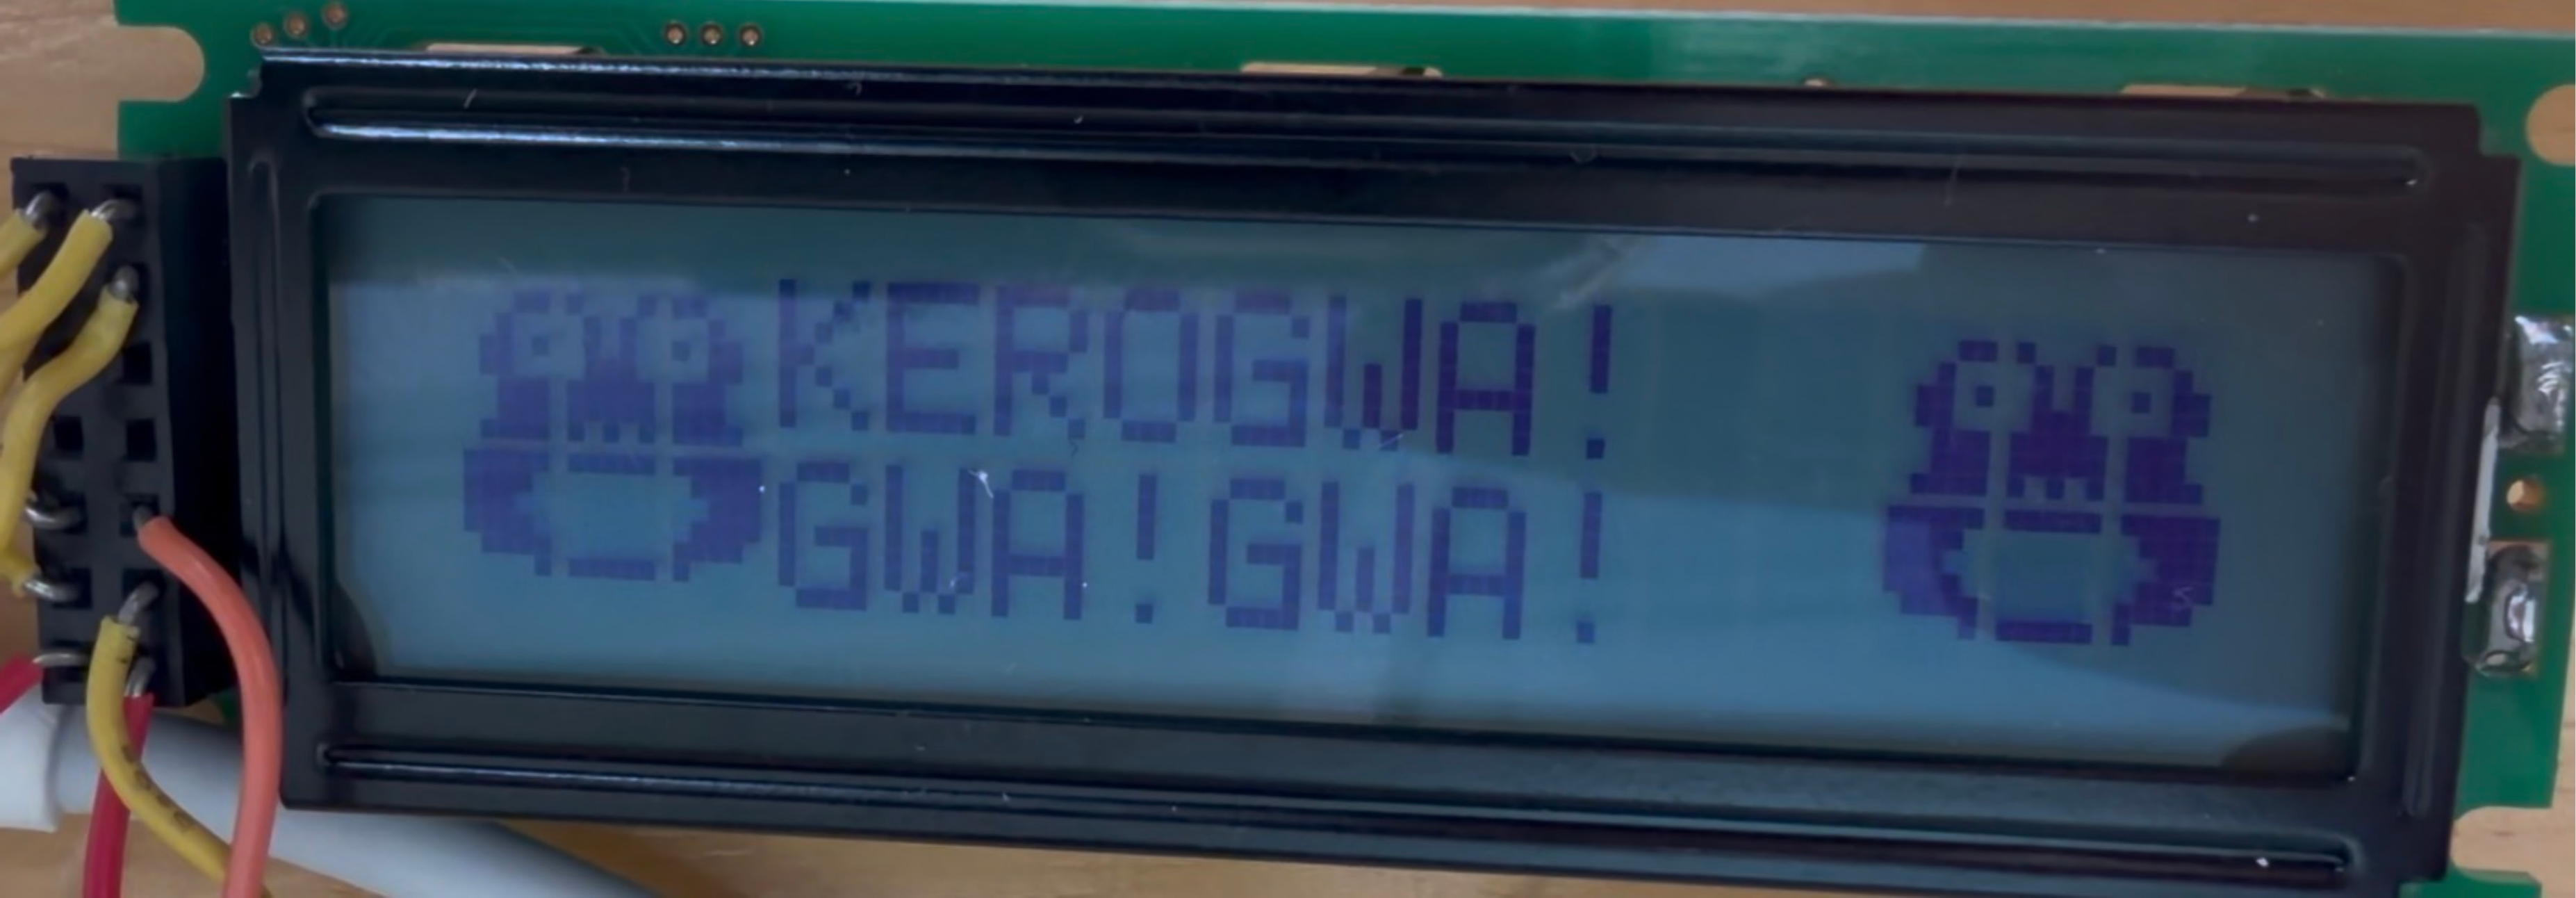
\includegraphics[width=0.85\linewidth]{lcd_img.png}
\end{center}
\caption{LCDに表示されたかえるのアニメーションと歌詞}
\label{fig:lcd}
\end{figure}



\subsection{主要な設計判断の整理}
\label{sec:decisions}

ここまでに述べたシステム構成は，開発の過程で行った複数の設計判断の結果である．主要な判断とその根拠を表\ref{tab:decisions}に整理する．各判断の詳細は表中で参照する節で述べる．

\begin{table}[H]
\caption{主要な設計判断と選定理由}
\label{tab:decisions}
\begin{center}
\footnotesize
\begin{tabular}{p{7em}p{7.5em}p{7.5em}p{11em}}
\hline
判断項目 & 採用した案 & 検討した代替案 & 選定理由 \\
\hline
同期の通信方式 & 赤外線ブロードキャスト & MIDI，Wi-Fi，BLE & 1対多の同時送信が本来の用途であり，通信インフラに依存しない（\ref{sec:sync-compare}節） \\
赤外線フォーマット & Sony SIRC 12ビット & NEC 32ビット & フレーム長が18.0\,msと68.1\,msで，目標30\,msを満たせるのは前者のみ（\ref{sec:proto-compare}節） \\
伝送する情報 & 参加楽器マスク4ビットのみ & 楽譜データの配信，tick番号の併送 & 通信量を子機の台数に依存させないため．ただし位置の自己修復を失う（\ref{sec:disc-mask}節） \\
楽譜の保持場所 & 各子機がプログラム内に保持 & 親機から毎tick配信 & 子機単体でのテストを可能にし，担当者ごとの並行開発を成立させるため \\
輪唱の開始方式 & 再生開始後の随時参加 & 押下順に固定の時間差を割り当てるカノン方式 & 任意の順・任意のタイミングで参加できる自由度を優先（\ref{sec:design-change}節） \\
参加の反映時点 & 次の8tick境界 & ボタンを押した瞬間 & 各声部の入りを拍に揃え，輪唱としてかみ合わせるため \\
退場の反映時点 & 参加時点から32tickの倍数境界 & ボタンを押した瞬間 & 旋律を途中で切らず1周弾き切ってから抜けるため \\
ピアノ音源の合成 & 倍音の加算合成 & サンプリング再生，物理モデル合成 & 音源データを使わず，実時間で扱える計算量に収めるため（\ref{sec:piano-compare}節） \\
ピアノ音源の再生 & 起動時の事前レンダリングとSampler & 発音のたびの実時間合成 & 発音時の処理を最小化し，合成の計算量が演奏タイミングへ影響しないようにするため（\ref{sec:piano}節） \\
テンポ変更の入力 & 可変抵抗による連続調整 & ボタンによる段階的な増減 & 演奏中のテンポ変化を滑らかにするため（\ref{sec:tempo}節） \\
親機の待機方式 & \texttt{millis()}による経過時間の監視 & \texttt{delay()}による待機 & 待機中もボタン入力と可変抵抗の読み取りを続けるため \\
\hline
\end{tabular}
\end{center}
\end{table}

このうち報告者が主体的に関与したのは，ピアノ音源の合成方式と再生方式，テンポ変更の入力方式，および輪唱の開始方式の試作である．報告者の担当部分がシステム全体の機能実現に果たす役割は次のように整理できる．ピアノは旋律を担う中心の楽器であり，その音色の再現性はMOE3（楽器音らしい音色である）に直結する．また事前レンダリング方式の採用は，発音時の処理時間を抑えることでMOE1（違和感なく聞くことができる）を支えている．テンポ管理は親機のtick周期そのものを決める機能であり，全子機の演奏速度を一括して制御するためMOE2（可変テンポに対応している）の実現手段そのものである．さらに，\ref{sec:bugfix}節で述べる2件の不具合修正は，いずれも輪唱が通しで成立するための前提条件であった．

\section{システム実装}
\label{sec:impl}

\subsection{チーム構成と役割分担}

本プロジェクトは6名で実施した．作業はProcessingでの音源作成，子機Arduinoのプログラム，親機Arduinoのプログラム，回路・表示装置の4系統に分け，WBSの管理番号を付けて分担した．役割分担を表\ref{tab:roles}に示す．報告者はピアノ音源の作成とそのArduino通信用関数，ドラムの子機プログラム，およびテンポ管理プログラムを担当した．テンポ管理は渡邊との共同である．第9週末までのチーム全体の作業時間は129時間であり，報告者の累計は35時間であった．

\begin{table}[H]
\caption{チームの役割分担}
\label{tab:roles}
\begin{center}
\small
\begin{tabular}{lll}
\hline
担当者 & WBS番号 & 主な担当 \\
\hline
櫛濵 和輝（報告者） & 110, 120, 240, 320 & ピアノ音源・通信関数，ドラム子機，テンポ管理（共同） \\
家田 祐希 & 130, 140, 220, 310 & フルート音源・通信関数・子機，赤外線管理（共同） \\
木下 遼介 & 150, 160, 230, 410 & トランペット音源・通信関数・子機，回路（共同） \\
久家 力孔 & 170, 171, 180 & ドラム音源（キック・シンバル），ドラム通信関数 \\
渡邊 乃斗 & 250, 310, 320 & 楽譜進行，赤外線管理（共同），テンポ管理（共同） \\
手代木 巧 & 410, 420 & 回路作成，LEDマトリクス・LCD表示 \\
全員 & 510, 520 & 輪唱機能の結合，結合テスト \\
\hline
\end{tabular}
\end{center}
\end{table}

開発は，第5週までを計画段階，第6週から第9週までを実装段階とし，第10週に統合と結合テストを行う計画で進めた．WBS第3層のタスク単位のスケジュールを図\ref{fig:gantt}に示す．タスク番号は表\ref{tab:roles}のWBS番号に対応する．

\begin{figure}[H]
    \begin{center}
    % 凡例
    \begin{tikzpicture}
      \fill[blue!40] (0,0) rectangle (0.4,0.3); \node[right,font=\footnotesize] at (0.5,0.15) {計画};
      \fill[yellow!50] (2.2,0) rectangle (2.6,0.3); \node[right,font=\footnotesize] at (2.7,0.15) {延長};
      \fill[green!50] (4.4,0) rectangle (4.8,0.3); \node[right,font=\footnotesize] at (4.9,0.15) {追加実装};
    \end{tikzpicture}
    \vspace{2pt}

    \begin{ganttchart}[y unit title=0.4cm,
    y unit chart=0.5cm,
    vgrid,hgrid,
    title label anchor/.style={below=-1.6ex},
    title left shift=.05,
    title right shift=-.05,
    title height=1,
    title/.append style={fill=yellow!10},
    progress label text={},
    bar height=0.7,
    bar label font=\footnotesize,
    group right shift=0,
    group top shift=.6,
    group height=.3]{1}{18}
    % ラベル
    \gantttitle{実装段階（第5週〜第10週）}{18} \\
    \gantttitle{W5}{3}
    \gantttitle{W6}{3}
    \gantttitle{W7}{3}
    \gantttitle{W8}{3}
    \gantttitle{W9}{3}
    \gantttitle{W10}{3}\\
    % タスク（仕様書に基づく更新版）
    \ganttbar[bar/.append style={fill=blue!40}]{110:ピアノ音の作成/櫛濵・久家}{1}{6} \\
    \ganttbar[bar/.append style={fill=blue!40}]{120:通信用関数（ピアノ）/櫛濵・久家}{4}{6} \\
    \ganttbar[bar/.append style={fill=blue!40}]{130:フルート音の作成/家田・渡邊}{1}{3} \\
    \ganttbar[bar/.append style={fill=blue!40}]{140:通信用関数（フルート）/家田・渡邊}{1}{3} \\
    \ganttbar[bar/.append style={fill=blue!40}]{150:トランペット音の作成/木下・手代木}{1}{3} \\
    \ganttbar[bar/.append style={fill=blue!40}]{160:通信用関数（トランペット）/木下・手代木}{1}{3} \\
    \ganttbar[bar/.append style={fill=blue!40}]{170:ドラム音の作成（キック）/櫛濵・久家}{4}{6} \\
    \ganttbar[bar/.append style={fill=blue!40}]{171:ドラム音の作成（シンバル）/櫛濵}{4}{6} \\
    \ganttbar[bar/.append style={fill=blue!40}]{180:通信用関数（ドラム）/久家}{4}{6} \\
    \ganttbar[bar/.append style={fill=blue!40}]{210:ピアノのプログラム/櫛濵}{7}{9} \\
    \ganttbar[bar/.append style={fill=blue!40}]{220:フルートのプログラム/家田}{7}{9} \\
    \ganttbar[bar/.append style={fill=blue!40}]{230:トランペットのプログラム/木下}{7}{9} \\
    \ganttbar[bar/.append style={fill=blue!40}]{240:ドラムのプログラム/櫛濵・久家}{10}{12}
    \ganttbar[bar/.append style={fill=yellow!50}]{}{13}{15} \\
    \ganttbar[bar/.append style={fill=blue!40}]{250:楽譜進行/家田・渡邊}{10}{12}
    \ganttbar[bar/.append style={fill=yellow!50}]{}{13}{15} \\
    \ganttbar[bar/.append style={fill=blue!40}]{310:赤外線管理/家田・渡邊}{13}{15} \\
    \ganttbar[bar/.append style={fill=blue!40}]{320:テンポ管理/家田・渡邊}{13}{15} \\
    \ganttbar[bar/.append style={fill=blue!40}]{410:回路作成/木下・手代木}{13}{15} \\
    \ganttbar[bar/.append style={fill=green!50}]{420:LEDマトリクス/木下・手代木}{16}{18} \\
    \ganttbar[bar/.append style={fill=green!50}]{510:結合機能作成/木下・手代木}{16}{18} \\
    \ganttbar[bar/.append style={fill=green!50}]{520:結合テスト/全員}{16}{18}
    \end{ganttchart}
    \end{center}
    \caption{開発スケジュール}
    \label{fig:gantt}
\end{figure}

図\ref{fig:gantt}のバーは計画時の週割当てである．110:ピアノ音の作成は第5週の仮実装と第7週の音色改善の2期間に分けて実施した．実施ではいくつかのタスクが計画より後ろへ延びており，420:LEDマトリクス作成は表示不具合の解消に時間を要して第10週まで作業が続いた．250:楽譜進行，310:赤外線管理，320:テンポ管理の3タスクも，第8週の結合テストで発覚した課題に対応するため第9週まで追加実装を行った．音源作成と通信用関数は計画通り第7週末までに完了している．

\subsection{親機Arduinoの処理}

親機は，演奏の開始とリセット，子機の参加と退場の予約，およびテンポの変更を受け付けながら，全子機に共通の時間基準となるtickを刻み，赤外線フレームを送信する指揮装置である．主要な関数を表\ref{tab:func_parent}に，loop()を1周する処理の流れを図\ref{fig:flow_parent}に示す．loop()では，シリアルコマンドと各ボタンの入力，および可変抵抗によるテンポ変更を毎周監視したうえで，再生中であれば前回のtickからの経過時間を調べ，式(\ref{eq:tick})のtick間隔$T_\mathrm{tick}$に達したときだけtick()を実行する．参加ボタンとそれに対応するシリアルコマンドはtoggleChildに集約されており，図\ref{fig:state}の状態遷移に従って予約とその取消が切り替わる．

tick()では，まず参加予約と退場予約が発火するtickに到達したかを子機ごとに判定して参加状態を更新し，参加中の子機集合を表すマスクを組み立てる．参加中の子機が1台でもあるときは，遅延計測用の同期パルスを出力したのち，tickカウンタの下位8ビットとマスクを赤外線の1フレームとして送信する．loop()の末尾では子機ボタン横のLEDを参加状態と予約の有無に同期させ，予約の取消を含むどの操作でも表示が確実に切り替わるようにしている．

\begin{table}[H]
\caption{親機Arduinoの主要関数}
\label{tab:func_parent}
\begin{center}
\small
\begin{tabular}{llp{15em}}
\hline
関数名 & 役割 & 概要 \\
\hline
\texttt{loop} & メインループ & 入力の監視とtick周期の管理を行い，子機LEDの表示を内部状態に同期させる \\
\texttt{handleSerialCommand} & シリアル入力の処理 & 1文字コマンドを解釈し，参加トグルや再生開始，リセットの各関数に振り分ける \\
\texttt{handleOrderButtons} & 参加ボタンの処理 & 子機ごとのボタンの立ち下がりを検出して\texttt{toggleChild}を呼び出す \\
\texttt{toggleChild} & 参加と退場の予約 & 子機の状態に応じて参加予約，退場予約，およびそれらの取消を切り替える \\
\texttt{handleTempoPot} & テンポの調整 & 可変抵抗の値を平滑化して読み取り，60〜150\,BPMの範囲でテンポを更新する \\
\texttt{doStart} & 再生の開始 & 全子機を未参加に初期化し，tickカウンタを0に戻して計時を開始する \\
\texttt{doReset} & リセット & 再生を停止し，全子機の参加状態とすべての予約を初期化する \\
\texttt{tick} & 同期信号の送信 & 予約の発火判定と参加マスクの生成を行い，赤外線フレームを送信する \\
\hline
\end{tabular}
\end{center}
\end{table}

\begin{figure}[H]
\begin{center}
\begin{tikzpicture}[
  term/.style={draw, rounded corners=8pt, minimum width=8em, minimum height=1.9em, align=center, font=\footnotesize},
  proc/.style={draw, minimum width=13em, minimum height=2.1em, align=center, font=\footnotesize},
  dec/.style={draw, diamond, aspect=2.6, align=center, font=\footnotesize, inner sep=1pt},
  lbl/.style={font=\footnotesize, inner sep=2pt},
  >=Stealth, node distance=0.5cm]
  \node[term] (start) {loop() の先頭};
  \node[proc, below=of start] (input) {シリアルコマンドと各ボタンの入力を監視し\\toggleChild / doStart / doReset を実行};
  \node[proc, below=of input] (pot) {可変抵抗の値を平滑化して読み取り\\tempoBpm を 60〜150\,BPM に更新};
  \node[dec, below=of pot] (playing) {isPlaying が真か};
  \node[dec, below=of playing] (interval) {$T_\mathrm{tick}$ が経過したか};
  \node[proc, below=of interval] (fire) {tick() を実行し，joinTick / leaveTick に到達した\\子機の参加状態を切り替えて参加マスク mask を生成};
  \node[dec, below=of fire] (mask) {mask が 0 以外か};
  \node[proc, below=of mask] (send) {同期パルスを出力し，sendNEC で\\tickCount の下位8ビットと mask を送信};
  \node[proc, below=of send] (inc) {tickCount をインクリメント};
  \node[proc, below=of inc] (led) {子機LEDを参加状態と予約の有無に応じて点灯};
  \node[term, below=of led] (loopend) {loop() の先頭へ戻る};

  \draw[->] (start) -- (input);
  \draw[->] (input) -- (pot);
  \draw[->] (pot) -- (playing);
  \draw[->] (playing) -- node[lbl, right] {Yes} (interval);
  \draw[->] (interval) -- node[lbl, right] {Yes} (fire);
  \draw[->] (fire) -- (mask);
  \draw[->] (mask) -- node[lbl, right] {Yes} (send);
  \draw[->] (send) -- (inc);
  \draw[->] (inc) -- (led);
  \draw[->] (led) -- (loopend);

  % tick を打たない経路（再生中でない，または tick 間隔が未経過）
  \coordinate (byp) at ($(interval.east)+(1.8,0)$);
  \draw[->] (playing.east) -- node[lbl, above] {No} (playing.east -| byp) |- (led.east);
  \draw (interval.east) -- node[lbl, above] {No} (byp);
  % 参加中の子機がいなければ送信を飛ばす経路
  \draw[->] (mask.east) -- node[lbl, above] {No} ++(1.2,0) |- (inc.east);
\end{tikzpicture}
\end{center}
\caption{親機Arduinoの処理フロー}
\label{fig:flow_parent}
\end{figure}


\subsection{子機Arduinoの処理}

子機Arduinoは，親機からの赤外線フレームを受けて自分のパートを演奏する側の装置である．楽譜のデータは通信では受け取らず，各子機が自分のパートの譜面配列をプログラム内に保持している．受信したマスクのうち自分の担当ビットが立っているtickだけを自分の出番と解釈し，出番の回数を数えるカウンタ\texttt{localPos}を1つ進めたうえで，譜面配列のその位置の音符情報をシリアル通信でProcessingへ送信する．親機の進行にはループの概念がないため，メロディ機は譜面の末尾に達したら\texttt{localPos}を0へ戻し，子機の側で先頭からの繰り返しを作る．ドラム機は譜面を持たず，出番のたびにキックの合図を送るだけである．子機のプログラムは4台で共通であり，冒頭の機体番号\texttt{childId}を書き換えて各機体へ書き込むことで，メロディ機3台とドラム機1台を作り分けている．

譜面位置24以降は，1tickにつき2音を発音する倍速区間である．旋律の終盤にあたるこの区間では，1音あたりの音長を通常の0.40\,sから0.20\,sへ半分にし，2音目を直近の受信間隔の半分だけ遅らせて送信することで，16分音符相当の刻みを作る．待ち時間の基準となる受信間隔は受信のたびに計測するが，演奏の停止と再開のあいだに生じる大きな間隔をそのまま使うと待ち時間が膨らむため，極端な値は捨てて更新する．また，この待ち時間の間にも次のフレームは届きうるので，受信データは復号した直後に退避して受信器をすぐに再開し，待機中も受信を続けてtickの取りこぼしを防いでいる．このほか，親機の同期パルスの立ち上がり時刻を割り込みで記録し，赤外線の受信までの遅延をログへ出力する計測の仕組みも子機側に持たせている．子機の主要な関数を表\ref{tab:func_child}に，\texttt{loop}の処理の流れを図\ref{fig:flow_child}に示す．

\begin{table}[H]
\caption{子機Arduinoの主要関数}
\label{tab:func_child}
\begin{center}
\small
\begin{tabular}{llp{15em}}
\hline
関数名 & 役割 & 概要 \\
\hline
\texttt{setup} & 初期化 & シリアル通信と赤外線受信を開始し，同期パルス入力の割り込みを登録する \\
\texttt{loop} & 受信監視と発音 & 赤外線フレームを常時監視し，自分の出番のtickで譜面位置を進めて音符情報を送信する \\
\texttt{sendNoteToHost} & 音符情報の送信 & 音高，音長，音量，譜面位置をカンマ区切りの1行にまとめてProcessingへ送る \\
\texttt{onSyncRise} & 同期パルスの記録 & 親機の同期パルスの立ち上がり時刻を記録する割り込み処理で，遅延計測の基準になる \\
\texttt{printReady} & 起動通知 & 起動時に自分の機体番号とメロディ機かドラム機かの種別をシリアルへ出力する \\
\hline
\end{tabular}
\end{center}
\end{table}

\begin{figure}[H]
\begin{center}
\begin{tikzpicture}[
  term/.style={draw, rounded corners=7pt, minimum width=6em, minimum height=1.9em, align=center, font=\footnotesize},
  proc/.style={draw, minimum height=1.9em, align=center, font=\footnotesize},
  dec/.style={draw, diamond, aspect=2.3, align=center, font=\footnotesize, inner sep=1pt},
  lbl/.style={font=\footnotesize, inner sep=2pt},
  >=Stealth, node distance=0.5cm]
  \node[term] (start) {起動};
  \node[proc, below=of start] (init) {シリアル通信と赤外線受信を初期化し\\同期パルス割り込みを登録（\texttt{setup}）};
  \node[proc, below=of init] (wait) {赤外線フレームの受信を待ち\\マスクを退避して受信を再開};
  \node[dec, below=of wait] (nec) {NECフォーマットか};
  \node[dec, below=of nec] (mine) {自分の担当ビットが\\立っているか};
  \node[proc, below=of mine] (adv) {出番の回数\texttt{localPos}を1進める};
  \node[dec, below=of adv] (drum) {ドラム機か};
  \node[dec, below=of drum] (loopchk) {\texttt{localPos}が楽譜1周分の\\32tickに達したか};
  \node[proc, below=of loopchk] (intv) {受信間隔を計測し\\半tick分の遅延時間を更新};
  \node[dec, below=of intv] (dbl) {譜面位置が24以降の\\倍速区間か};
  \node[proc, below=of dbl] (single) {譜面の音符を音長0.40\,sで\\Processingへ送信};
  \node[proc, right=0.9cm of loopchk] (reset) {\texttt{localPos}を0に戻し\\先頭からループ};
  \node[proc] (kick) at (reset.center |- drum.center) {キック合図C2を送信し\\LEDを点滅};
  \node[proc] (two) at (reset.center |- dbl.center) {1音目を音長0.20\,sで送信し\\半tick後に2音目を送信};
  \coordinate (lx) at (-3.6,0);
  \coordinate (rx) at (7.6,0);
  \draw[->] (start) -- (init);
  \draw[->] (init) -- (wait);
  \draw[->] (wait) -- (nec);
  \draw[->] (nec) -- node[lbl, right] {Yes} (mine);
  \draw[->] (mine) -- node[lbl, right] {Yes} (adv);
  \draw[->] (adv) -- (drum);
  \draw[->] (drum) -- node[lbl, right] {No} (loopchk);
  \draw[->] (loopchk) -- node[lbl, right] {No} (intv);
  \draw[->] (intv) -- (dbl);
  \draw[->] (dbl) -- node[lbl, right] {No} (single);
  \draw[->] (nec.west) -- node[lbl, above] {No} (nec.west -| lx) |- (wait.west);
  \draw[->] (mine.west) -- node[lbl, above] {No} (mine.west -| lx) |- (wait.west);
  \draw[->] (drum.east) -- node[lbl, above] {Yes} (kick.west);
  \draw[->] (loopchk.east) -- node[lbl, above] {Yes} (reset.west);
  \draw[->] (dbl.east) -- node[lbl, above] {Yes} (two.west);
  \draw[->] (reset.south) |- (intv.east);
  \draw (single.south) -- ++(0,-0.45) coordinate (m1);
  \draw (two.south) |- (m1);
  \draw[->] (m1) -- (m1 -| lx) |- (wait.west);
  \draw[->] (kick.east) -- (kick.east -| rx) |- (wait.east);
\end{tikzpicture}
\end{center}
\caption{子機Arduinoの処理フロー}
\label{fig:flow_child}
\end{figure}


\subsection{LCD表示の処理}
\label{sec:lcd-impl}

表示用の子機は，16文字2行のLCDキャラクタディスプレイ1枚に，左右のカエル2体と中央の歌詞を同時に表示する．表示例は図\ref{fig:lcd}に示したとおりである．カエルはHD44780のカスタム文字機能で作成した5$\times$8ドットのパターンを3列2行に並べて構成し，上段の3文字は固定の絵柄，下段の3文字を口の開いた絵柄と閉じた絵柄とで差し替えることで口パクを表現する．左のカエルを列0〜2に，右のカエルを列13〜15に配置し，その間の列3〜12の2行を歌詞表示エリアとした．HD44780が同時に登録できるカスタム文字は8種類までであるため，左右のカエルで同じ6種類の文字を共有し，2体の口が常に同じ形で動く構成としている．

表示の進行は親機の赤外線tickに同期させる．受信したマスクのうち担当ビットが立ったtickでのみ歌詞位置\texttt{localPos}を1つ進め，対応する語を表示すると同時に口の開閉を反転させる．歌詞は楽譜1周分の32\,tickと1対1に対応する文字列テーブルとして保持している．1語を書き込むたびに書き込み列を語長だけ進め，残り幅に収まらなくなったら下段へ改行し，下段も埋まったら歌詞エリアだけを空白で消去して先頭から書き直す．画面全体を消去せずエリアを限定して消すのは，カエルの絵柄を保持したまま歌詞だけを更新するためである．口パクの更新では，CGRAMを書き換えると表示中の文字の形も即座に変わるHD44780の性質を利用し，カーソルを左右のカエルの下段へ移動して6文字を書き直すだけで2体の口を同時に動かしている．主要な関数を表\ref{tab:lcd_func}に，処理の流れを図\ref{fig:flow_lcd}に示す．

表示子機が受信するフレームは演奏子機と同じものであり，\ref{sec:proto-compare}節で述べたSony SIRC 12ビットへの移行にあわせて受信処理も更新している．親機は参加中の子機が1台でもあれば毎tickフレームを送信するので，表示子機は演奏子機と同じ時間基準で歌詞と口パクを進められる．ただし表示子機も演奏子機と同様に受信回数で位置を数えるため，フレームを取りこぼすと歌詞の位置が1つ後方へずれたまま戻らない．この性質と対策は\ref{sec:disc-mask}節で演奏子機とあわせて論じる．

\begin{table}[tb]
\caption{LCD表示の主要関数}
\label{tab:lcd_func}
\begin{center}
\small
\begin{tabular}{llp{18zw}}
\hline
関数名 & 役割 & 概要 \\
\hline
\texttt{setup} & 初期化 & シリアル通信とLCDを初期化してカエルのカスタム文字6種を登録し，口を閉じた状態で描画したうえで赤外線受信を開始する \\
\texttt{loop} & 受信と進行 & 赤外線フレームを受信し，担当ビットが立っていれば歌詞位置を1つ進めて歌詞表示と口パクを実行する \\
\texttt{showLyric} & 歌詞表示 & 指定位置の語を歌詞エリアへ書き込み，行幅に収まらない場合は改行またはエリアの消去を行う \\
\texttt{clearLyricArea} & 歌詞エリアの消去 & 列3〜12の2行だけを空白で埋め，書き込み位置を先頭へ戻す \\
\texttt{updateFrogs} & 口パクの更新 & 開閉に応じた口のパターンをCGRAMへ登録し直し，左右のカエル6文字を書き直す \\
\hline
\end{tabular}
\end{center}
\end{table}

\begin{figure}[tb]
\begin{center}
\begin{tikzpicture}[
  term/.style={draw, rounded corners=8pt, minimum width=9em, minimum height=2.2em, align=center, font=\footnotesize},
  proc/.style={draw, minimum width=12em, minimum height=2.2em, align=center, font=\footnotesize},
  dec/.style={draw, diamond, aspect=2.2, align=center, font=\footnotesize, inner sep=1.5pt},
  lbl/.style={font=\footnotesize},
  >=Stealth, node distance=0.55cm]
  \node[term] (start) {起動};
  \node[proc, below=of start] (init) {LCDを初期化してカエルのカスタム文字を登録し，\\口を閉じた状態で描画して赤外線受信を開始};
  \node[term, below=of init] (wait) {赤外線フレームの受信を待つ};
  \node[dec, below=of wait] (dec1) {フレームを\\受信したか};
  \node[dec, below=of dec1] (dec2) {maskの担当\\ビットが1か};
  \node[proc, below=of dec2] (pos) {歌詞位置\texttt{localPos}を1つ進める};
  \node[dec, below=of pos] (dec3) {\texttt{localPos}が\\32\,tickに達したか};
  \node[proc, below=of dec3] (lyric) {\texttt{showLyric}で歌詞エリアに次の語を書き込み\\（行幅を超える場合は改行）};
  \node[proc, below=of lyric] (flip) {口の開閉フラグ\texttt{frogOpen}を反転し，\\\texttt{updateFrogs}で左右のカエルの口を書き換える};
  \node[proc, right=0.9cm of dec3] (reset) {\texttt{localPos}を0に戻し\\歌詞エリアを消去};
  \coordinate (lane) at (6.9, 0);
  \draw[->] (start) -- (init);
  \draw[->] (init) -- (wait);
  \draw[->] (wait) -- (dec1);
  \draw[->] (dec1) -- node[lbl, right] {Yes} (dec2);
  \draw[->] (dec2) -- node[lbl, right] {Yes} (pos);
  \draw[->] (pos) -- (dec3);
  \draw[->] (dec3) -- node[lbl, right] {No} (lyric);
  \draw[->] (lyric) -- (flip);
  \draw[->] (dec3.east) -- node[lbl, above] {Yes} (reset.west);
  \draw[->] (reset.south) |- (lyric.east);
  \draw[->] (dec1.west) -- node[lbl, above] {No} ++(-1.6,0) |- (wait.west);
  \draw[->] (dec2.west) -- node[lbl, above] {No} ++(-1.6,0) |- (wait.west);
  \draw[->] (flip.east) -- (lane |- flip.east) -- (lane |- wait.east) -- (wait.east);
\end{tikzpicture}
\end{center}
\caption{LCD表示子機の処理フロー}
\label{fig:flow_lcd}
\end{figure}


\subsection{報告者の担当範囲と技術的課題}

報告者の担当のうち，ピアノはこのシステムの旋律を担う中心の楽器である．また，テンポ管理と演奏進行の時間設計はすべての楽器に影響する．実装を進めるなかで，解決すべき課題は次の4点に整理された．

\begin{itemize}
\item 打鍵後に減衰していくピアノらしい音色を，音源データを使わずに合成で作ること
\item 発音時の処理遅延を抑え，演奏のタイミングを崩さないこと
\item 親機と子機の進行が食い違い，特定の音が周期的に抜けるバグを解消すること
\item 休符が休符として聞こえるように，音の余韻を制御すること
\end{itemize}

以降の節で，それぞれの課題への取り組みを順に述べる．開発にあたって利用した支援ツールと情報源，およびその検証の過程については第\ref{sec:tools}章にまとめる．

\subsection{ピアノ音源の実装}
\label{sec:piano}

ピアノの音は，多数の倍音が異なる速さで減衰していく音である．正弦波1本やオルガン風の持続音では鍵盤楽器に聞こえないため，物理的な性質を模した加算合成を実装した．ピアノ弦の倍音周波数は弦の剛性により整数倍からわずかに高い方へずれることが知られており\cite{fletcher}，この性質はインハーモニシティと呼ばれる\cite{nishiguchi}．$h$次倍音の周波数$f_h$を，基本周波数$f_s$とインハーモニシティ係数$B$を用いて
\begin{equation}
f_h = h f_s \sqrt{1 + B h^2}
\label{eq:inharmonicity}
\end{equation}
で計算する．$B$は音域に応じて変える量であり，本実装では基本周波数$f_0$を用いて$B = 2\times10^{-4} \times (f_0/261.6)^{0.8}$とした．すなわち中央ハ（261.6\,Hz）で$2\times10^{-4}$である．

この値は文献の実測値と比較しておく必要がある．Youngはグランドピアノとアップライトピアノ計8台を測定し，中央ハの第2倍音のずれが約1.2\,centになると報告している\cite{young1952}．これは$B \simeq 3.5\times10^{-4}$に相当し，本実装の値のおよそ1.8倍である．また音域依存についても，Youngは中央ハより上では8半音ごとに$B$が倍になる，すなわち1オクターブあたり約2.8倍になるとしているのに対し，本実装の$f_0^{0.8}$では1オクターブあたり約1.7倍にとどまる．

つまり本実装は，実際のピアノよりも非調和性を弱く，かつ音域による変化を緩やかに設定している．これは試聴を繰り返して決めた値であり，文献値から導いたものではない．合成音を単独で聴く条件では，非調和性を強めると倍音の唸りが目立って濁って聞こえたためこの値に落ち着いた．文献値に近づけた場合の聴感を比較検証することは今後の課題である．

倍音は10次まで重ね，$h$次倍音の振幅は$1/h^p$に比例させて高次ほど弱くする．指数$p$は低音域で0.9，高音域で1.4程度になるように基本周波数から連続的に決めた．

減衰のエンベロープは，打鍵直後の速い減衰とその後の緩やかな減衰の2段階を重ねた形とし，時刻$t$での振幅係数を
\begin{equation}
e(t) = 0.3\,e^{-t/0.12} + 0.7\,e^{-t/\tau_h}, \qquad
\tau_h = \frac{\tau_1}{1 + 0.6\,(h-1)}
\label{eq:envelope}
\end{equation}
とした．$\tau_1$は基本音の減衰時定数であり，残響の長さが低音ほど長くなるように音域から決める．式(\ref{eq:envelope})の$\tau_h$は次数とともに小さくなるので，高次倍音ほど速く消える．これは実際のピアノで打鍵直後は明るく，時間とともに丸い音色に変わっていく振る舞いに対応する．このほか，実機のピアノが1音あたり複数の弦を持つことを模して，音域に応じて1〜3本の弦をセント単位でわずかにずらして重ねた．さらに打鍵の瞬間のハンマーノイズとして，最初の15\,msだけローパスフィルタを通した雑音を加え，立ち上がり3\,msのアタックと，音長経過後に時定数0.15\,sで減衰するダンパーリリースを付けている．

もう1つの課題は発音遅延である．上記の合成をすべて発音のたびに計算すると，波形生成に時間がかかり演奏に間に合わないおそれがある．計算量を見積もると，1音の波形は音長0.40\,sに余韻0.8\,sを加えた1.2\,s分であり，標本化周波数44.1\,kHzでは52{,}920サンプルとなる．高音域では3本の弦それぞれに10次までの倍音を重ねるため，1音あたり$52{,}920 \times 3 \times 10 \simeq 1.59 \times 10^{6}$回の正弦波演算が必要になる．一方，発音の間隔は120\,BPMのtick間隔250\,ms，倍速区間では125\,msである．この時間内に約159万回の演算を確実に終える保証はない．そこで，楽譜に登場する6種類の音高と2種類の音長の組をProcessingの起動時にすべて波形として生成し，MinimのSamplerにキャッシュしておく方式にした．起動時に生成する波形は12種類，演算回数の合計は約$1.8 \times 10^{7}$回であるが，これは起動時に1度だけ実行すればよい．演奏中はキャッシュ済みSamplerのtrigger()を呼ぶだけなので，発音時の処理は音源データの再生と同じで済む．Samplerは同時6声まで発音できる設定とし，前の音の余韻と次の音が自然に重なるようにした．未登録の音高が届いた場合はその場で生成してキャッシュに加える安全網も設けている．なお，このピアノ音源は当初オルガン風の持続音で仮実装しており，第9週に本節で述べた合成方式へ差し替えた．差し替え時には楽譜で使う全音高について試聴による検証を行い，全ケースで楽器音として問題ないことを確認している．各波形生成部のコードは付録\ref{sec:codep-pde},\ref{sec:codef-pde},\ref{sec:codet-pde},\ref{sec:coded-pde},に示す．

\subsection{演奏進行の不具合修正}
\label{sec:bugfix}

結合テストの過程で，演奏の時間管理に関わる不具合を2件修正した．いずれも症状の観察からログで原因を絞り込んだもので，修正自体は小さいが，輪唱の成立には欠かせない修正だった．

1件目は，特定の位置の音が周期的に鳴らない症状である．旋律の途中，譜面位置16や24の音が数周に一度抜けて聞こえた．子機のシリアルログで譜面位置の進み方を追ったところ，親機は32tickを楽譜1周として進行しているのに対し，子機は1周を33tickと解釈していることが分かった．子機側でループ末尾の休みを表す定数を2tickとしていたため，旋律31tickとの合計が33tickになっていたのが原因である．この不整合が症状として現れる機序は次のとおりである．親機は32tickで楽譜1周を刻むのに対し，子機は33回の受信で1周とみなすため，1周を終えるごとに子機の譜面位置が親機の意図する位置より1tickずつ後方へずれていく．子機の譜面配列では末尾に休符が置かれているため，ずれが特定の位置に達したtickでは本来音があるはずの箇所で休符が参照され，音が抜けて聞こえる．ずれは1周あたり1tickずつ増えて32周で一巡するので，同じ位置の音が抜ける現象は32周ごとに再現する．120\,BPMでは1周が$32 \times 0.25 = 8\,\mathrm{s}$であるから，周期はおよそ4分16秒となる．症状が「数周に一度」に見え，短い試奏では気づきにくかったのはこのためである．この定数を1に修正して両者を32tickに統一し，症状は解消した．第9週の4子機実機テストでも再発していない．

2件目は，休符が休符として聞こえない問題である．本システムの音長の既定値は0.40\,sであり，120\,BPMでのtick間隔0.25\,sより長い．前の音の余韻が次のtickまで残るため，譜面上の休符Rのタイミングでも直前の音が鳴り続け，旋律の切れ目が埋まってしまっていた．そこでProcessing側で休符Rを受信した時点で，発音中の音を即時に停止する処理を入れた．オルガン風音源の時点ではnoteOff()の即時呼び出しとして実装し，ピアノ音源への差し替え後もSamplerのstop()で同じ動作を維持している．音が鳴っている最中に切る処理なので不自然に聞こえる心配があったが，ピアノのダンパーで音を止めた場合と似た切れ方になり，聴感上の違和感はなかった．

\subsection{テンポ管理}
\label{sec:tempo}

テンポ管理は，親機のtick周期を演奏中に変更する機能である．当初はボタンの押下でテンポを段階的に増減する方式を実装していたが，デモで聴かせる際にテンポが跳びとびに変わるのは不自然だったため，第9週に可変抵抗による連続調整へ変更した．10\,k$\Omega$のシングルターン可変抵抗をアナログ入力に接続し，読み値$v$（0〜1023）をテンポの範囲60〜150\,BPMへ線形に対応付ける．
\begin{equation}
\mathit{BPM}(v) = 60 + \left\lfloor \frac{(150-60)\,v}{1023} \right\rfloor
\label{eq:bpm}
\end{equation}
読み取りは50\,ms間隔とし，読み値のノイズによるテンポの揺れを抑えるため，
\begin{equation}
s_n = \frac{3\,s_{n-1} + v_n}{4}
\label{eq:ema}
\end{equation}
の指数移動平均で平滑化してから式(\ref{eq:bpm})に与える．親機のtick周期の計算は毎ループ現在のテンポ変数を参照しているため，平滑化後の値が変われば次のtickから反映される．

この平滑化が追従時間に与える影響は式(\ref{eq:ema})から見積もれる．$v$が階段状に変化したとき，$n$回目の読み取り後の$s_n$は最終値の$1-0.75^{n}$倍まで達する．読み取り間隔は50\,msであるから，63\,\%に達するのは約174\,ms後（$n \simeq 3.5$），95\,\%に達するのは約550\,ms後（$n = 11$）である．120\,BPMの1拍は500\,msであり，つまみを一気に回して大きくテンポを変えた場合には，95\,\%の反映までに1拍をわずかに超える計算になる．実機で1拍以内の追従を確認できたのは，つまみの操作が連続的で1回あたりの変化量が小さかったためと考えられる．追従の速さとテンポの安定性は平滑化係数を通じて背反の関係にあり，現在の値はデモでの操作感を優先して選んだものである．

シリアルモニタへのログ出力は2\,BPM以上変化したときに限定し，微小な揺らぎでログが埋まらないようにした．

なお，親機の進行処理はdelay()で待つのではなく，millis()で前回tickからの経過時間を監視する方式である．待ち時間の間もボタン入力と可変抵抗の読み取りを続ける必要があるためで，テンポ変更・参加操作・tick送信が互いをブロックしない構造になっている．

\subsection{輪唱開始方式の試作と設計変更}
\label{sec:design-change}

輪唱の開始方法については，開発の途中で設計を大きく変えた経緯がある．当初の計画では，演奏開始前にボタンで各楽器の順番を登録し，登録順に固定の時間差で追いかける方式を想定していた．報告者はこの系統の親機プログラムに対して，押下順に応じて各子機の出だしのずれを動的に割り当てる実装を試作した．子機固有の固定遅延値として持っていた配列を，押された順番$N$に対する割当$\{0, 8, 16, 20\}$\,tickへ読み替えることで，どのボタンを最初に押してもその楽器が先頭声部として位置0から歌い出す，本来のカノンの形を実現するものである．

一方で，チーム内の検討により，輪唱の定義は「固定順で参加する」ものではなく「任意の順・任意のタイミングで参加できる」べきだという結論になり，第7週末にアーキテクチャを再生開始後の随時参加ボタン方式へ変更した．この方式では子機は演奏していない間も常に曲位置を共有しているため，途中から参加しても，その時点の位置から自然に演奏へ加われる．押下順カノン方式の試作は採用に至らなかったが，2案を実機で比較したことで，随時参加方式の方が演奏デモとしての自由度が高いことを確認したうえで移行できた．最終版の親機プログラムはこの随時参加方式であり，報告者が試作で得た8tick境界への参加アライメントの考え方は，そのまま参加予約の量子化として引き継がれている．

\subsection{担当部分以外の実装と工夫}

システムの残りの部分について，チームの実装を概観する．赤外線管理プログラムは渡邊と家田が担当し，親機からマスクとtick番号を一斉送信する方式や，参加・退場をOFF・QUEUED・ACTIVEの3状態で管理する仕組みを実装した．楽譜進行プログラムは渡邊が担当し，スタート信号を受けたtickの記録と，現在のtickとの比較で出力音を決める機能を追加した．

フルートは家田の担当で，倍音構造とADSRの調整により息の混じった柔らかい音色を作り，アタックタイムを短くしてテンポへの追従性を改善した．トランペットは木下の担当で，倍音比とビブラートによる音色合成に加え，音の切り替え時に発生していたプチという雑音を，Minimの出力ラインに0.03\,sのフェードアウトを入れることで解消した．また，トランペット系ではArduinoから29音の楽曲データを一括送信するため，シリアル通信速度を921600\,bpsとして受信配列への格納を確認している．ドラム音源は久家の担当で，キックとシンバルの2種を合成し，Arduinoから受信した整数値で再生し分けるProcessingを実装した．回路と表示装置は手代木の担当で，親機・子機の回路作成と，LCD表示プログラムの作成を進めた．

回路面では，第6週に赤外線受光モジュールの故障が3台見つかり，新品への交換と動作確認を家田が行った．こうした部品不良の切り分けができたのは，受光モジュール単体の受信テストを単体テストとして分離していたためである．

\section{開発支援ツールと情報源の活用}
\label{sec:tools}

本章では，報告者が開発で利用した支援ツールと情報源，それらをどのような目的で用いたか，および生成された結果をどのように検証して採否を判断したかを述べる．

\subsection{利用したツールと情報源の一覧}

利用したツールと情報源を表\ref{tab:tools}に整理する．いずれについても，得られた内容をそのまま用いるのではなく，一次資料との突き合わせか実機での動作確認のいずれかを経てから採用することを原則とした．

\begin{table}[H]
\caption{利用した開発支援ツールと情報源}
\label{tab:tools}
\begin{center}
\footnotesize
\begin{tabular}{lp{9em}p{10em}p{10em}}
\hline
種別 & 対象 & 利用目的 & 検証の方法 \\
\hline
生成AI & 対話型の生成AI & ピアノ音源の合成コードの下書き，不具合の原因候補の列挙 & 文献による式の裏取り，実機での試聴，シリアルログによる動作確認 \\
学術文献 & Fletcherら\cite{fletcher}，Young\cite{young1952}，西口\cite{nishiguchi} & インハーモニシティと倍音減衰の物理的根拠の確認，係数$B$の実測値との照合 & 式(\ref{eq:inharmonicity})として実装し，係数を文献値と比較したうえで試聴により決定（\ref{sec:piano}節） \\
仕様資料 & SB-ProjectsのIR解説\cite{necfmt,sircfmt} & NECとSony SIRCのフレーム長の算出 & 算出値と実測の片道遅延を突き合わせ（表\ref{tab:latency-breakdown}） \\
ライブラリ文書 & IRremote\cite{irremote} & \texttt{sendSony}の引数仕様，プロトコル定数，フレーム終端判定の挙動 & 実機のシリアル出力で受信内容を確認 \\
公式文書 & Arduino Documentation\cite{arduinodoc} & \texttt{millis}，\texttt{micros}，\texttt{attachInterrupt}，\texttt{analogRead}の仕様確認 & 実機の動作と照合 \\
データシート & OSRB38C9AA\cite{osrb} & 受光モジュールのピン配置，電源電圧，キャリア周波数38\,kHz & 受信テストで動作確認，故障判定にも使用 \\
ライブラリ文書 & Minim\cite{minim} & \texttt{Sampler}，\texttt{Oscil}，\texttt{ADSR}の使い方 & Processing上で単体動作を確認 \\
\hline
\end{tabular}
\end{center}
\end{table}

表\ref{tab:tools}の3行目は，情報源を主体的に使った例として挙げておきたい．SB-Projectsの解説から読み取ったSony SIRCの単位時間とビット表現を用いて式(\ref{eq:len-sirc})を立て，フレーム長18.0\,msを算出した．この値を実測の片道遅延28.077\,msと突き合わせることで，差分10.1\,msが受信側の処理時間であることを特定できた（\ref{sec:eval-latency}節）．仕様資料の数値を鵜呑みにして「SIRCだから速い」と述べるのではなく，仕様から導いた予測と実測を比較することで，遅延の内訳という新しい情報が得られている．

\subsection{生成AIの利用手順と検証の方針}

生成AIは，主にピアノ音源の実装と不具合の原因究明の2つの場面で利用した．いずれの場面でも，生成された内容を直接採用することはせず，次の手順を踏んだ．

第1に，生成されたコードや提案の根拠となる技術的な前提を，一次資料で確認する．ピアノ音源であれば，倍音周波数が整数倍からずれるという前提が正しいかを文献\cite{fletcher,nishiguchi}で確認した．第2に，実機またはProcessing上で動作させ，意図した結果が得られるかを確かめる．音色であれば試聴，通信であればシリアルログでの確認である．第3に，得られた結果が不十分であれば，どの部分が原因かを切り分けたうえで修正する．音色を決めるパラメータ類は，この段階で試聴を繰り返しながら手動で調整した．

この手順を踏んだ理由は，生成AIの出力が「もっともらしいが検証されていない」状態で提示されるためである．とくに音色の合成では，コードが文法的に正しく動作しても，出てくる音が目的の楽器に聞こえるとは限らない．コードが動くことと目的を達成することは別であり，前者だけを確認して採用することは避けた．

\subsection{生成結果を修正して採用した事例}

ピアノ音源の加算合成では，生成AIに倍音の加算による減衰音の下書きを作らせたうえで，次の2点を自分で修正した．

1点目は倍音の振幅配分である．下書きでは$h$次倍音の振幅を一律に$1/h$としていた．これを実装して試聴したところ，低音域では問題ないものの，高音域で倍音が強く残り金属的な響きになった．実際のピアノでは高音域ほど倍音が少なく基音が支配的になる．そこで振幅を$1/h^p$とし，指数$p$を低音域で0.9，高音域で1.4程度になるよう基本周波数から連続的に決める形に変更した（\ref{sec:piano}節）．

2点目は減衰の形である．下書きでは全倍音に共通の単一の指数減衰を用いていたが，これでは打鍵直後から音が消えるまで音色が変わらず，ピアノらしく聞こえなかった．西口が整理しているとおり，実際のピアノでは倍音ごとに減衰時定数が異なる\cite{nishiguchi}．そこで式(\ref{eq:envelope})のように，速い減衰と緩やかな減衰の2段階を重ねたうえで，時定数$\tau_h$を次数$h$とともに小さくすることで，時間経過とともに音色が丸くなる振る舞いを再現した．

いずれの修正も，文献が示す物理的な性質と実機での試聴結果の両方に基づいている．生成された下書きは実装の出発点としては有用であったが，そのままでは目的とする音色に達していなかった．

\subsection{生成結果を採用しなかった事例}

採用を見送った提案もある．ここでは2件を挙げる．

1件目は，ピアノ音源の再生方式である．初期の案は，フルートやトランペットと同様にMinimの\texttt{Oscil}と\texttt{ADSR}を組み合わせ，発音のたびに実時間で合成する構成であった．しかしピアノは10次までの倍音に加えて1音あたり最大3本の弦を重ねるため，1回の発音で生成する正弦波の本数がフルートやトランペットの数倍になる．発音のたびにこの計算を行うと，演奏のタイミングに間に合わない可能性があった．そこで実時間合成を採らず，楽譜に登場する音高と音長の組をProcessingの起動時にすべて波形として生成し，\texttt{Sampler}にキャッシュしておく事前レンダリング方式へ変更した（\ref{sec:piano}節）．発音時の処理を\texttt{trigger()}の呼び出しだけに減らすことで，合成の計算量が演奏タイミングへ影響しない構成としている．

2件目は，休符が休符として聞こえない問題への対処である．\ref{sec:bugfix}節で述べたとおり，この問題は音長の既定値0.40\,sがtick間隔0.25\,sより長いために生じていた．対処として音長そのものを短くする案も検討したが，音長を短くすると休符でない箇所でも音が早く切れ，旋律が痩せて聞こえる．そこで音長は保ったまま，休符Rを受信した時点で発音中の音を停止する処理を入れる方式を採った．実際のピアノでダンパーが弦の振動を止める動作に相当し，聴感上の違和感がないことを試聴で確認している．

これらの判断はいずれも，提案の内容を理解したうえで，本システムの制約（Processingの処理能力，tick間隔と音長の関係）に照らして下したものである．

\subsection{不具合の原因究明における利用}

\ref{sec:bugfix}節で述べたtick数不整合のバグでは，「特定の位置の音が数周に一度抜ける」という症状から考えられる原因候補を生成AIに列挙させた．挙がった候補は，赤外線フレームの取りこぼし，Processing側のシリアルバッファの詰まり，親機と子機の定数の不一致などであった．

これらを1つずつシリアルログで検証した．子機の譜面位置の進み方を追ったところ，親機が32\,tickを楽譜1周としているのに対し子機が33\,tickと解釈していることが判明し，定数の不一致が原因であると特定できた．候補の列挙は切り分けの出発点として有用であったが，どの候補が正しいかを決めたのはログという実データである．

なお，このとき否定した「赤外線フレームの取りこぼし」という候補は，当時の症状の原因ではなかったものの，後の定量計測（\ref{sec:eval-latency}節）で0.26\,\%の頻度で実在することが分かった．症状の原因ではないことと，現象が存在しないことは別である．この点は，原因候補を消去する際に「今回の症状を説明できるか」と「そもそも起きているか」を区別すべきだという教訓として残った．

\section{評価方法と結果}
\label{sec:eval}

\subsection{評価方法}

本システムの評価は，計画段階で定義した有効性指標（MOE），性能指標（MOP），技術性能指標（TPM）に基づいて行う．有効性指標MOEを表\ref{tab:moe}に示す．

\begin{table}[H]
\caption{有効性指標（MOE）の定義}
\label{tab:moe}
\begin{center}
\small
\begin{tabular}{ll}
\hline
MOE & 有効性指標 \\
\hline
MOE1 & 違和感なく聞くことができる \\
MOE2 & 可変テンポに対応している \\
MOE3 & 楽器音らしい音色である \\
MOE4 & 歌詞・アニメーションが演奏に対応している \\
\hline
\end{tabular}
\end{center}
\end{table}

各MOEに対応する性能指標MOPを表\ref{tab:mop}に定めた．MOE1にはMOP1（演奏タイミング誤差）とMOP2（同期信号の受信成功率）が，MOE2にはMOP3（テンポ変更への追従時間）が，MOE3にはMOP4（音色の再現性）が，MOE4にはMOP5（歌詞・アニメーション同期遅延）がそれぞれ対応する．

ここでMOP1の定義に注意が必要である．計画段階でのMOP1は「各演奏側Arduino間の音符開始タイミングのずれ」，すなわち\textbf{機器間の相対的なずれ}として定義した．親機の送信から子機の受信までに要する片道の時間はMOP1ではなく，プロジェクト中に監視する技術性能指標TPM1（赤外線通信遅延）として別に定義している．この2つは物理的に異なる量であり，混同すると評価の意味が変わってしまう．本報告書では両者を区別し，TPM1として計測した片道遅延の統計から，MOP1が満たされているかを論証する形をとる．MOPとTPMの対応を表\ref{tab:mop}および表\ref{tab:tpm}に示す．

MOP1の目標値30\,msは，実演奏のアンサンブルにおける奏者間の発音タイミングのずれがおよそ30〜50\,msの範囲に収まるというRaschの報告\cite{rasch}を根拠とする．MOP5の目標値55\,msは，音と映像のずれの知覚に関する報告\cite{arrighi}と，アンサンブル演奏における音の遅延条件の検討\cite{nagao2012}に基づいて定めた．音と映像の同期については視聴者が同時と感じる範囲を概ね100\,ms以内とする整理もある\cite{kuwahara2019}が，本システムでは口パクと発音が1対1に対応し，ずれが検知されやすいと判断してより厳しい55\,msを採用した．

\begin{table}[H]
\caption{性能指標MOPと目標値}
\label{tab:mop}
\begin{center}
\footnotesize
\begin{tabular}{llp{11em}p{10em}}
\hline
MOP & 性能指標 & 目標値（計画段階での定義） & 計測方法 \\
\hline
MOP1 & 演奏タイミング誤差 & 演奏側Arduino間の音符開始タイミングの差が30\,ms以内 & TPM1の統計から上界を評価 \\
MOP2 & 同期信号の受信成功率 & 送信に対する正しい受信の割合が95\,\%以上 & 送信回数と受信回数の比較 \\
MOP3 & テンポ変更への追従時間 & 全演奏側が1拍以内に追従 & シリアルモニタでの確認 \\
MOP4 & 音色の再現性 & 聴衆の過半数が対応する楽器の音と判断 & 5段階のアンケート \\
MOP5 & 歌詞・アニメーション同期遅延 & 演奏とLCD表示の差が55\,ms以内 & 演奏の動画からのフレーム差分 \\
\hline
\end{tabular}
\end{center}
\end{table}

\begin{table}[H]
\caption{監視した技術性能指標TPMと本報告書での扱い}
\label{tab:tpm}
\begin{center}
\footnotesize
\begin{tabular}{llp{16em}}
\hline
TPM & 監視項目 & 本報告書での扱い \\
\hline
TPM1 & 赤外線通信遅延 & 親機の送信から子機の受信復号完了までの片道遅延として計測し，\ref{sec:eval-latency}節で統計を示す \\
TPM2 & 同期信号受信率 & MOP2の評価にそのまま用いる \\
TPM3 & Processing音声再生遅延 & 事前レンダリング方式の採用により発音時の処理を最小化（\ref{sec:piano}節），定量計測は未実施 \\
TPM4 & LCD表示遅延 & MOP5の評価にそのまま用いる \\
TPM5 & CPU負荷・メモリ使用量 & コンパイル時のメモリ使用量で監視，定量計測は未実施 \\
\hline
\end{tabular}
\end{center}
\end{table}

検証は単体テスト，結合テスト，システムテストの3段階で計画した．単体テストでは各音源と通信機能を個別に確認し，結合テストでは親機・子機間の同期と子機・Processing間の接続を確認する．システムテストでは全構成を接続して課題曲の通し演奏を行う．

\subsection{単体テストの結果}

第5週から第8週にかけて実施した単体テストの結果を表\ref{tab:tests}に示す．音源系では，フルートの音色聴感テスト，トランペットの音色合成テストと切り替えノイズテスト，ドラムの単体再生テストがそれぞれ完了した．トランペットの切り替えノイズは，フェードアウト処理の追加によってテスト上で雑音が確認されなくなり，MOP4（音色の再現性）に関連する問題点として管理していたものが解消された．通信系では，921600\,bpsでのシリアル通信テストで29音の楽曲データが欠落なく受信・格納されることを確認した．また，赤外線受光モジュールの故障3台の交換後に受信テストを再実施し，回路の正常動作を確認している．ピアノ音源は差し替えの際に，楽譜で使う全音高と2種類の音長の組について試聴で確認した．

\begin{table}[H]
\caption{テストの実施結果}
\label{tab:tests}
\begin{center}
\small
\begin{tabular}{llll}
\hline
実施日 & テスト内容 & 結果 & 備考 \\
\hline
5/20〜5/25 & フルート音色聴感テスト & 成功 & 倍音構造・ADSR調整完了 \\
5/26 & トランペット音色合成テスト & 成功 & 倍音比とビブラートの確定 \\
5/26 & 音切り替えノイズテスト & 成功 & 0.03\,sフェードアウトで雑音解消 \\
5/26 & シリアル通信テスト（921600\,bps） & 成功 & 29音を欠落なく受信 \\
6月初旬 & ドラム音色単体テスト & 成功 & キック・シンバルの再生確認 \\
6/17 & 受光モジュール交換後の通信テスト & 成功 & 故障3台を交換 \\
6/19 & 3子機の輪唱テスト & 部分成功 & ドラムを除く3楽器で動作 \\
6/23 & 4子機の輪唱実機テスト & 成功 & 音抜け・休符抜けの再発なし \\
7月中旬 & 全構成でのシステムテスト & 成功 & 表示子機を含む全モジュールが同期動作 \\
\hline
\end{tabular}
\end{center}
\end{table}

\subsection{結合テストとシステムテストの結果}

結合テストは2段階で行った．第7週末の3子機テストでは，ピアノ・フルート・トランペットの3楽器での輪唱開始を実機で確認した．この時点ではドラムが未結合であり，部分成功という扱いである．続く第9週の6月23日に，親機1台と子機4台の全構成による輪唱の実機テストを実施した．ボタンの押下順にピアノ・フルート・トランペット・ドラムが順次参加するカノン演奏を通しで行い，聴感上の破綻なく演奏できることを全員で確認した．\ref{sec:bugfix}節で述べた位置抜けと休符抜けは，このテストで再発していない．参加・退場のトグル操作についても，予約とその取消，途中退場後の再参加が状態表示LEDの点灯と一致して動作した．

システムテストは，最終発表でのデモンストレーションとして実施した．親機1台，演奏子機4台，表示子機，および楽器音を再生するPC 4台を接続した全構成で「かえるのうた」の輪唱を通しで演奏し，ボタン操作による楽器の参加と退場，可変抵抗によるテンポの変更，LCDの歌詞表示と口パクアニメーションのすべてが正常に動作することを確認した．図\ref{fig:system}に示した構成のうち，結合テストの段階では未接続だった表示子機を含め，全モジュールが同一の赤外線tickに同期して動作したことになる．MOE1からMOE4までの有効性指標は，このシステムテストをもって達成と判断した．

テンポ管理については，可変抵抗のつまみ操作で演奏中のテンポが60〜150\,BPMの範囲で連続的に変わることを確認した．式(\ref{eq:tick})のtick周期は毎ループ現在のテンポを参照するため，追従の遅れはつまみ読み取りの平滑化に伴う数百ms程度であり，1拍以内というMOP3の目標を満たす動作である．ただしこの追従時間もログからの定量値としては算出しておらず，シリアルモニタ上の値の変化と聴感での確認にとどまっている．

\subsection{赤外線同期の定量評価}
\label{sec:eval-latency}

\subsubsection{計測方法}

赤外線同期の性能を計測するため，親機と子機の双方に計測用の機構を実装した．親機は赤外線フレームを送信する直前に同期パルス用の端子を立ち上げる．子機はこのパルスの立ち上がりを外部割り込みで捉えて\texttt{micros()}による時刻を記録し，赤外線フレームの復号が完了した時点との差を片道遅延としてシリアルへ出力する．この片道遅延がTPM1（赤外線通信遅延）にあたる．

7月13日に，この機構を有効にしたまま親機1台と子機1台を接続し，演奏状態のままtickを刻み続けて10{,}323\,tick分のログを取得した．計測時のtick間隔は，限られた時間で試行回数を確保するため実演奏時の250\,ms（120\,BPM）より短い50\,msに設定している．総計測時間は520.9\,sであった．時刻の記録に用いた\texttt{micros()}の分解能は4\,$\mu$sであり，以下に示す統計量の桁数はこの分解能に対して十分である．図\ref{fig:timing}に，1回のtickにおける時間の流れと計測区間の対応を示す．

\begin{figure}[H]
\begin{center}
\begin{tikzpicture}[>=Stealth, font=\footnotesize]
  % 時間軸
  \draw[->] (0,0) -- (13.2,0) node[right] {時間};
  \foreach \x/\t in {0/0, 4.5/18.0, 7.0/28.1} {
    \draw (\x,-0.12) -- (\x,0.12);
    \node[below, font=\scriptsize] at (\x,-0.15) {\t};
  }
  \node[below, font=\scriptsize] at (2.2,-0.62) {[ms]};
  % 親機の行
  \node[left, font=\scriptsize] at (0,1.35) {親機};
  \draw[dashed, gray] (0,0.2) -- (0,1.9);
  \fill[blue!25, draw=blue!60!black] (0,1.1) rectangle (0.25,1.6);
  \node[above, font=\scriptsize, align=center] at (0.35,1.62) {同期パルス};
  \fill[blue!35, draw=blue!60!black] (0,0.45) rectangle (4.5,0.95);
  \node[font=\scriptsize] at (2.25,0.7) {Sony SIRC 12ビットの送信 18.0\,ms};
  % 子機の行
  \node[left, font=\scriptsize] at (0,-1.35) {子機};
  \draw[dashed, gray] (4.5,-1.9) -- (4.5,0.2);
  \draw[dashed, gray] (7.0,-1.9) -- (7.0,0.2);
  \fill[orange!30, draw=orange!70!black] (4.5,-1.15) rectangle (7.0,-0.65);
  \node[font=\scriptsize, align=center] at (5.75,-0.9) {終端判定と復号\\10.1\,ms};
  \fill[green!25, draw=green!50!black] (7.0,-1.15) rectangle (10.0,-0.65);
  \node[font=\scriptsize, align=center] at (8.5,-0.9) {シリアル送信と\\Processingでの発音};
  % 計測区間
  \draw[<->, thick, red!70!black] (0,-1.65) -- (7.0,-1.65);
  \node[below, font=\scriptsize, red!70!black] at (3.5,-1.62) {TPM1として計測した片道遅延（実測 平均28.077\,ms）};
\end{tikzpicture}
\end{center}
\caption{1tickにおける時間の流れと計測区間の対応}
\label{fig:timing}
\end{figure}

\subsubsection{片道遅延の統計}

取得した10{,}323件の片道遅延の統計を表\ref{tab:sync-result}に，分布を図\ref{fig:hist}に示す．平均は28.077\,ms，標準偏差は0.137\,msであり，全体の99.88\,\%が28.2\,ms以下に収まった．

\begin{table}[H]
\caption{片道遅延（TPM1）の統計（$n=10{,}323$）}
\label{tab:sync-result}
\begin{center}
\small
\begin{tabular}{lrlr}
\hline
統計量 & 値 [ms] & 統計量 & 値 [ms] \\
\hline
平均 & 28.077 & 最小値 & 27.980 \\
中央値 & 28.072 & 最大値 & 34.688 \\
標準偏差 & 0.137 & 第99百分位 & 28.120 \\
外れ値を除く平均 & 28.072 & 外れ値を除く標準偏差 & 0.021 \\
\hline
\end{tabular}
\end{center}
\end{table}

\begin{figure}[H]
\begin{center}
\begin{tikzpicture}
\begin{axis}[
  width=0.86\linewidth, height=5.4cm,
  xlabel={片道遅延 [ms]}, ylabel={頻度 [回]},
  xmin=27.95, xmax=28.21, ymin=0, ymax=5200,
  ybar interval, ybar interval=0.92,
  tick label style={font=\footnotesize},
  label style={font=\small},
  xtick={27.98,28.02,28.06,28.10,28.14,28.18},
  xticklabel style={/pgf/number format/fixed, /pgf/number format/precision=2},
  ]
\addplot[fill=blue!35, draw=blue!60!black] coordinates {
(27.98,3) (28.00,26) (28.02,392) (28.04,2309) (28.06,4823) (28.08,1364)
(28.10,1256) (28.12,130) (28.14,7) (28.16,1) (28.18,0)};
\end{axis}
\end{tikzpicture}
\end{center}
\caption{片道遅延の分布（$n=10{,}323$，階級幅0.02\,ms，28.2\,msを超える12件は範囲外）}
\label{fig:hist}
\end{figure}

図\ref{fig:hist}が示すとおり，遅延は28.0〜28.2\,msの幅0.2\,msの範囲にほぼすべてが集中している．28.2\,msを超えたのは12回（0.116\,\%）であり，このうち1回は起動直後の初回受信（34.688\,ms）である．残る11回は30.8〜31.9\,msの範囲に集まっている．これら12件を除いた10{,}311件では標準偏差が0.021\,msとなり，これは時刻記録に用いた\texttt{micros()}の分解能4\,$\mu$sの数倍にすぎない．すなわち本システムの片道遅延は，測定分解能に近い精度で\textbf{一定値}とみなせる．

\subsubsection{遅延の内訳と仕様値との対応}

実測値28.077\,msが何によって決まっているかを検討する．計測時に参加していた子機は1台であり，このときのマスク値は0x01であるから，式(\ref{eq:len-sirc})において$k=1$として$L_\mathrm{SIRC}=30T=18.0\,\mathrm{ms}$となる．実測値との差は10.1\,msである．

この差は受信側の処理に起因する．IRremoteは，最後のマークの後にスペースが一定時間続いたことをもって1フレームの終端と判定するため，フレームの最終ビットが届いてから復号が始まるまでに待ち時間が生じる\cite{irremote}．これに\texttt{loop()}が周回して\texttt{decode()}が呼ばれるまでの時間と，復号処理そのものの時間が加わる．重要なのは，この10.1\,msが\textbf{フレーム長に依存しない固定量}である点である．したがってプロトコルをさらに短いフォーマットに変更しても，片道遅延を10\,ms程度より小さくすることはできない．遅延の内訳を表\ref{tab:latency-breakdown}に整理する．

\begin{table}[H]
\caption{片道遅延の内訳}
\label{tab:latency-breakdown}
\begin{center}
\small
\begin{tabular}{lrl}
\hline
区間 & 時間 [ms] & 根拠 \\
\hline
Sony SIRC 12ビットの送信 & 18.0 & 式(\ref{eq:len-sirc})に$k=1$を代入した仕様値 \\
受信側の終端判定・復号・ループ周回 & 10.1 & 実測値との差として算出 \\
\hline
合計（片道遅延） & 28.1 & 実測平均 28.077\,ms \\
\hline
\end{tabular}
\end{center}
\end{table}

\subsubsection{外れ値の原因}

28.2\,msを超えた11回（起動直後の1回を除く）について，発生したtickの譜面位置を調べたところ，いずれも譜面位置24以降の倍速区間であり，具体的には位置25，28，30，32のいずれかであった．倍速区間では1tickにつき2音を送信するため，子機は1音目を送信した後に半tick分待機してから2音目を送信する．この待機とシリアル送信の処理が次のフレームの復号と重なると，\texttt{decode()}が呼ばれるまでの時間が延びる．増加分が約3.8\,msでほぼ一定していることも，偶発的な擾乱ではなく特定の処理経路との競合であることを裏づけている．倍速区間は楽譜1周32\,tickのうち9\,tick，すなわち28\,\%の時間しか占めないにもかかわらず外れ値が集中していることから，この解釈は妥当と考える．

\subsubsection{受信成功率（MOP2）}

受信成功率は2つの方法で評価した．第1に，結合テストにおいて親機から一定間隔で100回送信し，子機が正しく受信した回数を数えた．結果は100回中100回の成功であり，計画段階で定めた「100回中95回以上」を満たした．

第2に，前述の演奏ログから受信の抜けを推定した．子機は受信した回数で譜面位置を進めるため，位置の連続性からは抜けを検出できない．そこで受信間隔に着目した．計測時のtick間隔は50\,msであるから，フレームを1つ取りこぼすと受信間隔が約100\,msに伸びる．10{,}322回の受信間隔のうち，99〜101\,msとなったものが27回あった．演奏の中断による2.56\,sの間隔1回を除くと，欠落率は$27/10{,}322 = 0.26\,\%$，受信成功率は99.74\,\%となる．結果を表\ref{tab:recv-result}に示す．

\begin{table}[H]
\caption{同期信号の受信成功率（MOP2）の評価結果}
\label{tab:recv-result}
\begin{center}
\small
\begin{tabular}{lllc}
\hline
評価方法 & 試行数 & 結果 & 判定 \\
\hline
結合テスト（100回送信） & 100 & 100回受信（100\,\%） & 達成 \\
演奏ログからの推定 & 10{,}322 & 欠落27回（99.74\,\%） & 達成 \\
\hline
\end{tabular}
\end{center}
\end{table}

100回の試行では欠落が観測されず，10{,}000回規模の試行で初めて0.26\,\%の欠落が現れた．計画段階で定めた100回の試行では，本システムの受信成功率を1\,\%の桁で評価することはできなかったことになる．試行回数を2桁増やしたことで，目標は依然として満たしつつも，無視できない頻度で欠落が生じるという実態が把握できた．欠落の原因については\ref{sec:disc-loss}節で論じる．

\subsubsection{演奏側Arduino間の相対ずれ（MOP1）の評価}

MOP1は演奏側Arduino間の音符開始タイミングの差である．本システムでは親機が1つのフレームを全子機へ同時にブロードキャストするため，子機間の受信時刻の差は，各子機における片道遅延の差にそのまま等しい．子機のプログラムは4台で共通であり，受光モジュールと配線も同一構成であるから，各子機の片道遅延は同じ分布に従うとみなせる．

この分布の標準偏差は外れ値を除いて0.021\,ms，外れ値を含めても0.137\,msである．最も保守的に，2台の子機の一方が観測された最小値27.980\,msを，他方が最大値34.688\,msを示した場合を考えても，その差は6.708\,msにとどまる．したがって子機間の相対ずれは最悪でも6.7\,ms，通常は0.1\,ms未満であり，MOP1の目標である30\,ms以内を大きく下回る．評価結果を表\ref{tab:mop1-result}に示す．

\begin{table}[H]
\caption{演奏タイミング誤差（MOP1）の評価結果}
\label{tab:mop1-result}
\begin{center}
\small
\begin{tabular}{lll}
\hline
評価の観点 & 値 & 目標30\,msとの関係 \\
\hline
片道遅延の標準偏差（外れ値を除く） & 0.021\,ms & 通常時の子機間ずれの目安 \\
片道遅延の標準偏差（全データ） & 0.137\,ms & 外れ値を含む場合の目安 \\
観測された最大値と最小値の差 & 6.708\,ms & 最悪ケースの上界 \\
\hline
\end{tabular}
\end{center}
\end{table}

ただしこの評価は，1台の子機で得た片道遅延の分布から他の子機の挙動を推定したものであり，複数の子機を同時に接続して受信時刻の差を直接計測したものではない．この点は評価手法の限界であり，\ref{sec:disc-eval-limit}節で改めて論じる．

\subsection{音色の評価（MOP4）}

楽器音の音色は，Googleフォームで作成したアンケートを用いて学科内で調査した．各楽器音を単独で再生した音声を提示し，「対応する楽器の音に聞こえるか」を5段階で回答してもらう形式である．回答者は18人であった．結果を表\ref{tab:tone-result}および図\ref{fig:tone}に示す．

\begin{table}[H]
\caption{音色の評価結果（18人アンケート，5段階評価）}
\label{tab:tone-result}
\begin{center}
\small
\begin{tabular}{llll}
\hline
楽器音 & 評価平均 & 4以上の割合 & 判定 \\
\hline
ピアノ & 3.78 & 61.1\,\%（11/18人） & 達成 \\
フルート & 4.33 & 83.3\,\%（15/18人） & 達成 \\
トランペット & 3.61 & 61.1\,\%（11/18人） & 達成 \\
キック & 3.72 & 61.1\,\%（11/18人） & 達成 \\
シンバル & 4.00 & 66.7\,\%（12/18人） & 達成 \\
\hline
\end{tabular}
\end{center}
\end{table}

\begin{figure}[H]
\begin{center}
\begin{tikzpicture}
\begin{axis}[
  width=0.86\linewidth, height=5.2cm,
  ybar=2pt, bar width=9pt,
  ymin=0, ymax=5.4,
  ylabel={5段階評価の平均}, ylabel style={font=\small},
  symbolic x coords={ピアノ,フルート,トランペット,キック,シンバル},
  xtick=data,
  tick label style={font=\footnotesize},
  nodes near coords, nodes near coords style={font=\scriptsize},
  every node near coord/.append style={/pgf/number format/fixed, /pgf/number format/precision=2},
  legend style={font=\footnotesize, at={(0.5,-0.18)}, anchor=north, legend columns=2, draw=none},
  ]
\addplot[fill=blue!35, draw=blue!60!black] coordinates {
  (ピアノ,3.78) (フルート,4.33) (トランペット,3.61) (キック,3.72) (シンバル,4.00)};
\addlegendentry{評価平均}
\addplot[sharp plot, no markers, dashed, red!70!black, line width=0.9pt, nodes near coords={}] coordinates {
  (ピアノ,3.0) (フルート,3.0) (トランペット,3.0) (キック,3.0) (シンバル,3.0)};
\addlegendentry{尺度の中央値（3.0）}
\end{axis}
\end{tikzpicture}
\end{center}
\caption{楽器音ごとの5段階評価の平均（$n=18$）}
\label{fig:tone}
\end{figure}

MOP4の判定基準である「4以上の割合が過半数」は全5音色で満たしており，目標を達成した．一方で評価平均には音色による差があり，フルートの4.33に対してトランペットは3.61，報告者が担当したピアノは3.78にとどまった．フルートが高い評価を得たのは，基音が支配的で高次倍音が弱いという音色の特徴が，倍音構造とADSRエンベロープという単純な合成モデルに素直に対応するためと考えられる．これに対しトランペットの金管特有の輝きや，ピアノの打鍵時の複雑な過渡音は，倍音の加算だけでは再現しきれない成分を含む．

なお，この評価には手法上の限界がある．回答者18人は同一学科の学生であり，楽器音の聴取に習熟した集団ではない．また各楽器音を単独で提示しているため，実際の合奏の中でどう聞こえるかは評価できていない．提示順序の効果も統制していない．これらの点については\ref{sec:disc-eval-limit}節で改めて述べる．

\subsection{LCD表示同期の評価（MOP5）}

LCD表示と演奏の同期は，演奏中のシステム全体を動画で撮影し，発音のタイミングとLCDの表示更新が現れるフレームの差から算出した．結果を表\ref{tab:lcd-result}に示す．同期誤差は約50.1\,msであり，目標の55\,ms以内を満たした．

\begin{table}[H]
\caption{LCD同期の評価結果}
\label{tab:lcd-result}
\begin{center}
\small
\begin{tabular}{llll}
\hline
評価項目 & 目標 & 結果 & 判定 \\
\hline
LCD同期誤差 & 55\,ms以内 & 約50.1\,ms & 達成 \\
\hline
\end{tabular}
\end{center}
\end{table}

ただしこの値は目標値55\,msに対する余裕が4.9\,msと小さく，計測手法の分解能を考えると判定は慎重に扱う必要がある．動画のフレーム差分による計測では，フレームレートが分解能の下限を決める．一般的な30\,fpsの撮影であれば1フレームは33.3\,msに相当し，この手法で0.1\,ms単位の値を分離することはできない．したがって「約50.1\,ms」という値は，実質的には「1〜2フレーム程度のずれ」を意味すると解釈すべきである．赤外線同期に用いたようなシリアルログによる時刻比較を行えば，マイクロ秒単位での評価が可能である．この点は\ref{sec:disc-eval-limit}節で論じる．

\subsection{評価結果の総括}

各指標の評価結果を表\ref{tab:overall-result}にまとめる．MOP1からMOP5までのすべてで目標を達成した．

\begin{table}[H]
\caption{性能指標の達成状況}
\label{tab:overall-result}
\begin{center}
\footnotesize
\begin{tabular}{llp{13em}c}
\hline
指標 & 目標値 & 結果 & 判定 \\
\hline
MOP1 & 演奏側間のずれ30\,ms以内 & 片道遅延の標準偏差0.021\,ms，最悪ケースでも6.708\,ms & 達成 \\
MOP2 & 受信成功率95\,\%以上 & 100回試行で100\,\%，10{,}322回試行で99.74\,\% & 達成 \\
MOP3 & テンポ追従1拍以内 & 実機で1拍以内に追従（実測値は未取得） & 達成 \\
MOP4 & 過半数が4以上と評価 & 全5音色で過半数を達成（平均3.61〜4.33） & 達成 \\
MOP5 & LCD同期55\,ms以内 & 約50.1\,ms（計測分解能に留意） & 達成 \\
\hline
\end{tabular}
\end{center}
\end{table}

ただし達成の確からしさは指標ごとに異なる．同期・通信に関するMOP1とMOP2は10{,}000回規模の試行に基づく統計として確度が高い一方，MOP3は実測値を取得しておらず，MOP4とMOP5には計測手法に起因する限界が残る．この差については\ref{sec:disc-eval-limit}節で整理する．

\section{考察}
\label{sec:discuss}

\subsection{一律の遅延とばらつきの区別}
\label{sec:disc-jitter}

\ref{sec:eval-latency}節で得た2つの数値，すなわち片道遅延の平均28.077\,msと標準偏差0.021\,msは，同期性能の議論において全く異なる意味を持つ．この区別が本システムの評価の中心にある．

平均28.077\,msは，親機がtickを刻んでから子機が音を出すまでの一律の遅れである．この遅れはすべての子機に等しく現れるため，演奏全体が28\,ms遅れて始まるだけであり，パート間のずれとしては現れない．これに対し標準偏差0.021\,msは，その遅れが受信のたびにどれだけばらつくかを表す．合奏が崩れて聞こえる原因は，パート間の相対的なずれである．Raschが報告した30〜50\,msという値も，演奏全体の遅れではなく奏者間の相対的なずれについてのものである\cite{rasch}．

したがって，片道遅延の平均値28.077\,msを目標値30\,msと直接比較して達成を主張する扱い方は，論証として適切ではない．両者は一律の遅れと相対的なずれという異なる量であり，仮に片道遅延が100\,msであっても，そのばらつきが十分小さければ合奏は成立する．本報告書が\ref{sec:eval-latency}節でばらつきの統計を評価の中心に置いたのは，この理由による．

この観点に立つと，本システムの同期性能は目標に対して大きな余裕を持つ．標準偏差0.021\,msは目標値30\,msの約1/1400である．この余裕は，赤外線のブロードキャストが本質的に1対多の同時送信であり，各子機が同一の物理信号を同時に受け取ることに由来する．Wi-FiやBLEのようにパケットが機器ごとに個別配送される方式では，配送時刻が機器ごとに異なるため，この性質は得られない．\ref{sec:sync-compare}節で赤外線を選定した判断は，同期精度という観点からは結果的に有利に働いたといえる．

なお，28\,msの一律遅延が無害であると結論づけるには条件がある．演奏者がボタンを押してから音に反映されるまでの応答としては知覚されうるからである．ただし本システムでは参加の反映を8\,tick境界まで待つ設計としており，120\,BPMではこの待ち時間が最大2\,sに達する．28\,msはこれに比べて2桁小さく，操作感には影響しない．

\subsection{受信欠落の原因と影響の見積り}
\label{sec:disc-loss}

\ref{sec:eval-latency}節で得た0.26\,\%という欠落率について，原因と影響を検討する．

まず発生位置に偏りがある．欠落27回のうち12回が譜面位置24以降の倍速区間で発生した．倍速区間は楽譜1周32\,tickのうち9\,tickであり，時間としては28\,\%を占めるにすぎないから，44\,\%という発生割合は偏りとみてよい．倍速区間では2音目の送信のために子機が半tick分待機するため，この間に到来したフレームを取りこぼしやすいと考えられる．外れ値の発生位置も同じ倍速区間に集中していたことと整合する．

次に，計測条件が欠落率を押し上げている可能性がある．計測時のtick間隔は50\,msであり，片道遅延28.1\,msはその56\,\%を占める．次のフレームが到来するまでの余裕は約22\,msしかない．実演奏の120\,BPMではtick間隔が250\,msとなり余裕は222\,msに広がるため，欠落率はこれより低くなると推定される．ただし実演奏のテンポでのログは取得していないため，この推定は検証されていない．

欠落が演奏に与える影響は，本方式の構造上，一過性では済まない．子機は受信した回数で自分の譜面位置を進めるため，1回の欠落がそのまま1\,tickの位置ずれとして以後も残り続ける．計測時の欠落率0.26\,\%をそのまま当てはめると，楽譜1周32\,tickあたりの期待欠落回数は$32 \times 0.0026 = 0.083$回であり，およそ12周に1回の割合で位置ずれが生じる計算になる．120\,BPMでは1周が8\,sであるから，約1分36秒に1回である．第9週の実機テストで破綻が観測されなかったのは，1回の通し演奏がこれより短かったためと考えられる．長時間の連続演奏では顕在化する問題であり，\ref{sec:disc-mask}節で述べる自己修復機構が必要となる根拠でもある．

\subsection{マスク方式の有効性と設計上のトレードオフ}
\label{sec:disc-mask}

本システムの同期方式は，楽譜データを通信せず，参加楽器のマスクだけを毎tick送るものである．4子機の実機テストで輪唱が破綻なく成立したことから，この情報量の絞り込みは有効だったと考える．Sony SIRC 12ビットの1フレームに必要な情報がすべて収まるため，子機の台数を増やしてもフレーム長も送信頻度も変わらない．コマンド部7ビットのうち下位4ビットをマスクに使用しているので，上位3ビットも活用すれば理論上は7台までこの構成のまま拡張できる．楽譜を子機に分散させたことは，通信量の削減だけでなく，子機単体でのテストを可能にするという開発上の利点もあった．各楽器の担当者が自分の子機とProcessingだけで音源の開発を進められたのは，この構成によるところが大きい\cite{kobayashi2013}．

一方で，この構成は\ref{sec:proto-compare}節で述べたプロトコル移行との間にトレードオフを生んでいる．NECフォーマットを用いていた時期には，アドレス部8ビットにtick番号の下位8ビットを載せることができたため，子機は受信のたびに自分の譜面位置を絶対値として復元でき，1回の受信失敗は次の受信で自動的に回復した．Sony SIRC 12ビットへの移行により片道遅延は68.1\,msから28.1\,msへ短縮されたが，コマンド7ビットとアドレス5ビットにtick番号を載せる余地はなく，位置の自己修復機能は失われた．その結果が\ref{sec:disc-loss}節で見積もった位置ずれの蓄積である．

この2つを両立させる方法は残されている．マスクに使うのは下位4ビットであり，コマンド部の上位3ビットが空いている．ここにtick番号の下位3ビットを載せれば，子機は自分の位置を8\,tick周期の中で照合でき，1回の欠落であれば次の受信で検出・修正できる．8\,tickは参加予約の量子化単位と一致するため，実装上の整合もとりやすい．子機を最大4台に制限する代わりに位置の自己修復を得るという選択であり，本システムの構成では妥当な交換だと考える．今後の改善点の中では優先度が最も高い．

\subsection{tick数不整合の教訓}

\ref{sec:bugfix}節の位置抜けバグは，親機と子機が「楽譜1周分のtick数」という同じ意味の値を，別々のファイルに別々の定数として持っていたことが根本原因である．修正は定数1つの変更で済んだが，症状は数周に一度しか現れないため，原因の特定には子機のログから位置の進み方の周期性を読み取る必要があった．親機32に対して子機33という1tickの差は，単体テストでは決して現れず，実機で長く演奏して初めて聞こえてくる．設計書に定数の対応関係を明記して両側から参照すること，そして結合した状態で数周分を通しで聴くテストを早い段階に置くことが，同種の不整合への対策になると考える．

\subsection{音長の固定値とテンポ可変の関係}

休符抜けの問題は，音長の既定値0.40\,sがtick間隔0.25\,sより長いという時間設計の矛盾から生じた．休符受信時の即時停止で聴感上は解消したが，これは対症的な処置でもある．本システムはテンポを60〜150\,BPMまで連続可変としたので，tick間隔は式(\ref{eq:tick})より500\,msから200\,msまで変わる．音長を固定値のままにすると，遅いテンポでは音符間に隙間が生まれ，速いテンポでは余韻の重なりが増える．音長をtick間隔に比例させて，テンポに追従した長さで発音する方式が本質的な改善になる．子機は直近の受信間隔を計測して倍速区間の遅延に使っており，この値を音長の算出にも流用できるはずである．

\subsection{ピアノ音源の方式選択}

ピアノ音源で採った事前レンダリング方式は，音色の複雑さと発音遅延の両立という点でうまく働いた．発音時の処理がSamplerのtrigger()だけになるため，加算合成の計算量が演奏タイミングへ影響しない．一方でこの方式には，音高・音長・音量の組ごとに波形を持つ必要があるという制約がある．今回の楽曲は6音高$\times$2音長で済んだが，曲目を増やすならキャッシュの生成時間とメモリが増えていく．また，打鍵の強弱で音色が変わるベロシティ表現は現状持っていない．強弱を数段階の波形として持つか，再生時の音量係数で近似するかは，音質と資源のトレードオフとして今後検討したい．

\subsection{評価手法そのものの限界}
\label{sec:disc-eval-limit}

本システムは5つの性能指標すべてで目標を達成したが，達成の確からしさは指標ごとに異なる．評価を主張する以上，この差を明示しておく必要がある．

MOP1については，1台の子機で得た片道遅延の分布から，子機間の相対ずれの上界を推定した．この推定は「4台の子機が同一の物理信号を同時に受け取る」という構成上の性質と，「4台のプログラムとハードウェアが同一である」という事実に依拠している．論理としては妥当だが，複数の子機を同時に接続して受信時刻の差を直接計測したわけではない．直接計測するには，各子機の発音信号を1つのロジックアナライザまたはオシロスコープの複数チャンネルで同時に観測すればよく，計画段階でもこの方法を想定していた．機材の都合で実施できなかったことが，本評価の最大の弱点である．

MOP2については，計画段階で定めた100回の試行では欠落が1回も観測されず，受信成功率を1\,\%の桁で評価できなかった．試行回数を10{,}000回規模へ増やしたことで0.26\,\%という欠落率が初めて把握できた．目標値が95\,\%であるのに対し試行回数が100回では，判定に必要な分解能に対して試行が2桁足りていなかったことになる．指標の目標値と試行回数の対応は，計画段階で検討すべき事項であった．

MOP3については，可変抵抗の操作に対してテンポが追従することを聴感とシリアルモニタで確認したにとどまり，追従時間を直接計測していない．\ref{sec:tempo}節では式(\ref{eq:ema})の平滑化から95\,\%到達までを約550\,msと見積もったが，これは計算による推定であって実測値ではない．つまみを一気に回した場合には120\,BPMの1拍500\,msをわずかに超える可能性があり，実測による確認が必要である．テンポ変更の指令時刻とtick間隔が実際に変化した時刻をログに出力すれば計測できる．

MOP4については，回答者18人が同一学科の学生であり，楽器音の聴取に習熟した集団ではない．また各音色を単独で提示しているため，合奏の中での聞こえ方は評価できていない．提示順序による効果も統制していない．18人という標本数では，音色間の平均値の差（フルート4.33とトランペット3.61）が偶然の範囲を超えるかどうかも判定できない．

MOP5については，動画のフレーム差分という手法の分解能が問題になる．30\,fpsの撮影では1フレームが33.3\,msに相当し，「約50.1\,ms」という値は実質的に1〜2フレームのずれを意味する．目標値55\,msとの差は4.9\,msであり，この差は手法の分解能より小さい．赤外線同期の計測と同様にシリアルログで時刻を比較すれば，マイクロ秒単位での評価が可能である．

以上をまとめると，MOP1とMOP2は10{,}000回規模の統計に基づく確かな評価である一方，MOP3からMOP5については計測手法の改善余地が残る．本システムの中心的な機能である同期性能について確度の高い評価ができた点は評価計画の成果であるが，周辺機能の評価手法には計画段階からの検討不足があったといえる．

\subsection{システムの限界と改善案}
\label{sec:disc-limit}

本システムに残された課題を，優先度の順に整理する．

第1に，\ref{sec:disc-mask}節で述べた譜面位置の自己修復である．受信欠落が1\,tickの位置ずれとして蓄積する現在の構造は，長時間の連続演奏で必ず顕在化する．コマンド部の空き3ビットにtick番号の下位3ビットを載せる改修により対処できる見込みであり，改修の規模も小さい．

第2に，\ref{sec:disc-eval-limit}節で述べた評価手法の改善である．とくにMOP1の直接計測は，本システムの主張の中核に関わるため優先度が高い．

第3に，Sony SIRCがエラー検出を持たないことによる耐ノイズ性の未検証である．屋内での計測では10{,}000回規模の試行で0.26\,\%の欠落にとどまったが，これは蛍光灯や日射による赤外線ノイズが少ない環境での値である．屋外や強い照明下での動作は確認していない．

第4に，機能面の拡張として，楽譜が子機のプログラムに固定配列として埋め込まれている点が挙げられる．楽譜データを外部から書き換えられる形式にすれば，同じハードウェア構成のまま演奏曲を増やせる．

このほか，報告者の担当範囲では，\ref{sec:tempo}節で述べた音長の固定値をtick間隔に比例させる改修と，ピアノ音源へのベロシティ表現の追加が残っている．

\section{おわりに}

本プロジェクトでは，複数の機器をリアルタイムに同期させる仕組みを合奏という題材で実現することを目的として，赤外線によるマスク同期を用いたArduino輪唱演奏システムを制作した．楽曲データを通信せず参加楽器のマスク4ビットのみを毎tick送る構成により，「かえるのうた」の輪唱を成立させ，演奏者がボタンで各楽器を任意のタイミングで参加・退場させること，および可変抵抗によるテンポの連続調整を実現した．最終発表でのシステムテストでは，親機・演奏子機4台・表示子機・PC 4台の全構成が同一の赤外線tickに同期して動作し，演奏，参加と退場の操作，テンポ変更，LCDの歌詞表示と口パクのすべてが正常に機能することを確認した．

序論で示した5つの定量目標に対する達成状況は次のとおりである．第1の目標である演奏側Arduino間の音符開始タイミングのずれ30\,ms以内については，10{,}323\,tick分のログから片道遅延の標準偏差が0.021\,ms（外れ値を含めても0.137\,ms）であることを示し，最悪ケースの上界6.708\,msをもって達成を確認した．第2の受信成功率95\,\%以上については，100回試行で100\,\%，10{,}322回試行で99.74\,\%を得て達成した．第3のテンポ変更への1拍以内の追従，第4の音色が過半数に楽器音と認識されること，第5のLCD表示同期55\,ms以内についても，それぞれ目標を満たした．

これらの達成を支えたのは，\ref{sec:proto-compare}節で述べた赤外線フォーマットの選定である．NECフォーマットではフレーム送信だけで68.1\,msを要し目標を単独で超過するのに対し，Sony SIRC 12ビットでは18.0\,msに短縮され，受信側の固定処理時間10.1\,msを加えた28.1\,msで安定した．さらに，赤外線ブロードキャストが全子機へ同一の物理信号を同時に届ける性質により，遅延のばらつきが測定分解能に近い水準に収まった．合奏の同期で問題になるのは一律の遅れではなく機器間の相対的なずれであるという\ref{sec:disc-jitter}節の整理に立てば，この性質こそが本方式の本質的な利点である．

報告者は，倍音の加算合成と事前レンダリングによるピアノ音源，ドラム子機のプログラム，可変抵抗によるテンポ管理を実装し，親機と子機のtick数不整合による周期的な音抜けと，音の余韻による休符抜けの2つの不具合を修正した．

残された課題として最も優先度が高いのは，コマンド部の空き3ビットを用いた譜面位置の自己修復である．受信欠落0.26\,\%はおよそ12周に1回の位置ずれとして蓄積するため，長時間の演奏では対処が必要になる．次いで，表示子機のプロトコルをSony SIRCへ更新すること，MOP1を複数子機の同時計測で直接検証すること，そして音長のテンポ追従とピアノ音源のベロシティ表現が挙げられる．

\section{変更履歴}

本報告書の主要な変更履歴を表\ref{tab:changelog}に示す．

\begin{table}[H]
\caption{主要な変更履歴}
\label{tab:changelog}
\begin{center}
\small
\begin{tabular}{lll}
\hline
日付 & 種別 & 変更内容 \\
\hline
5/13 & 設計 & 赤外線通信方式の基本設計を策定 \\
5/20 & 実装 & フルート音色の聴感テスト完了 \\
5/26 & 実装 & トランペット音色合成テスト完了 \\
5/26 & 修正 & トランペット音切り替えノイズを解消（0.03\,sフェードアウト） \\
5/26 & 実装 & シリアル通信テスト（921600\,bps）完了 \\
6月初旬 & 実装 & ドラム音色（キック・シンバル）単体テスト完了 \\
6/17 & 修正 & 赤外線受光モジュール故障3台を交換・動作確認 \\
6/19 & テスト & 3子機での輪唱テスト（部分成功） \\
6/23 & テスト & 4子機の輪唱実機テスト成功 \\
6月下旬 & 修正 & tick数不整合バグを修正（子機33tick→32tick） \\
6月下旬 & 修正 & 休符が聞こえない問題を修正（即時停止処理追加） \\
6月下旬 & 設計変更 & 輪唱開始方式を押下順カノンから随時参加方式へ変更 \\
7月初旬 & 実装 & ピアノ音源をオルガン風から加算合成方式へ差し替え \\
7月初旬 & 実装 & テンポ管理をボタン式から可変抵抗式へ変更 \\
7月初旬 & 実装 & LCD表示プログラムの統合 \\
7/8 & 計測 & 音色アンケート実施（18人，5段階評価） \\
7/8 & 計測 & LCD同期誤差の計測（約50.1\,ms，動画フレーム差分法） \\
7/13 & 計測 & 同期・通信の定量評価実施（片道遅延 平均28.077\,ms，標準偏差0.137\,ms，10{,}323\,tick分のログ） \\
7月中旬 & テスト & 最終発表で全構成のシステムテストを実施（表示子機を含め正常動作） \\
\hline
\end{tabular}
\end{center}
\end{table}

\clearpage
\begin{thebibliography}{99}
%% 同期・音響に関する学術文献
\bibitem{rasch} Rasch, R. A., ``Synchronization in performed ensemble music,'' Acustica, Vol.43, No.2, pp.121--131, 1979.
\bibitem{fletcher} Fletcher, H., Blackham, E. D. and Stratton, R., ``Quality of Piano Tones,'' The Journal of the Acoustical Society of America, Vol.34, No.6, pp.749--761, 1962. \url{https://doi.org/10.1121/1.1918192}
\bibitem{young1952} Young, R. W., ``Inharmonicity of Plain Wire Piano Strings,'' The Journal of the Acoustical Society of America, Vol.24, No.3, pp.267--273, 1952. \url{https://doi.org/10.1121/1.1906888}
\bibitem{nishiguchi} 西口磯春，``ピアノの音響とその物理モデル,'' RISTニュース，一般財団法人高度情報科学技術研究機構，No.56，pp.25--35，2014. \url{https://www.rist.or.jp/rnews/56/56s4.pdf}
\bibitem{arrighi} Arrighi, R., Alais, D. and Burr, D., ``Perceptual synchrony of audiovisual streams for natural and artificial motion sequences,'' Journal of Vision, Vol.6, No.3, Article 6, pp.260--268, 2006. \url{https://doi.org/10.1167/6.3.6}
\bibitem{kuwahara2019} 桑原圭裕，``映像と音の同期 ---「動画先行の原則」の根拠と応用,'' 映像学，Vol.102，pp.54--74，2019. \url{https://doi.org/10.18917/eizogaku.102.0_54}
\bibitem{nagao2012} 長尾翼 他，``音の遅延条件がアンサンブル演奏に与える影響に関する検討,'' 日本音響学会研究発表会講演論文集，pp.997--998，2012年3月.
%% 通信規格・技術資料
\bibitem{midi} 一般社団法人音楽電子事業協会（AMEI），``MIDI規格委員会,'' \url{https://amei.or.jp/midistandardcommittee/}，参照 2026年6月.
\bibitem{necfmt} SB-Projects, ``IR Remote Control Theory: NEC Protocol,'' \url{https://www.sbprojects.net/knowledge/ir/nec.php}，参照 2026年5月.
\bibitem{sircfmt} SB-Projects, ``IR Remote Control Theory: Sony SIRC,'' \url{https://www.sbprojects.net/knowledge/ir/sirc.php}，参照 2026年7月.
\bibitem{irremote} Shirriff, K.（原作），Joachimsmeyer, A.（保守），``IRremote Arduino Library,'' \url{https://github.com/Arduino-IRremote/Arduino-IRremote}，参照 2026年5月.
\bibitem{minim} Di Fede, D., ``Minim: An audio library for Processing,'' \url{http://code.compartmental.net/minim/}，参照 2026年5月.
\bibitem{arduinodoc} Arduino, ``Arduino Documentation,'' \url{https://docs.arduino.cc/}，参照 2026年5月.
\bibitem{osrb} OptoSupply International Ltd., ``7.4$\times$6.2$\times$5.25\,mm Infrared Receiver Module OSRB38C9AA データシート,'' \url{https://akizukidenshi.com/goodsaffix/OSRB38C9AA.pdf}，参照 2026年6月.
%% 組込み・IoT教育に関する文献
\bibitem{sakamura2017} 別所正博，坂村健，``INIAD：IoT時代の新しい学び舎,'' 情報の科学と技術，Vol.67，No.11，pp.582--588，2017. \url{https://doi.org/10.18919/jkg.67.11_582}
\bibitem{igaki2018} 井垣宏，武元貴一，上田悠貴，``基礎的なIoT教育のためのチーム開発を重視したPBL授業の提案,'' コンピュータソフトウェア，Vol.35，No.1，pp.1\_54--1\_66，2018.
\bibitem{yoshikawa2021} 吉川祐樹，川勝望，林和彦，``全学科全学年に横断したPBL型授業による学生の主体性の向上について,'' 工学教育，Vol.69，No.2，pp.2\_2--2\_10，2021. \url{https://doi.org/10.4307/jsee.69.2_2}
\bibitem{noguchi2020} 野口孝文，布施泉，千田和範，稲守栄，``IoT機能を持つロボットを用いた協調学習環境,'' 教育システム情報学会誌，Vol.37，No.2，pp.106--119，2020. \url{https://doi.org/10.14926/jsise.37.106}
\bibitem{kobayashi2013} 小林敬太，佐藤賢文，神戸英利，三井浩康，``学生を対象とした組込みソフトウェア技術者育成のためのHW/SWトレードオフ実験方式,'' 工学教育，Vol.61，No.4，pp.4\_36--4\_42，2013. \url{https://doi.org/10.4307/jsee.61.4_36}
\bibitem{kato2019} 加藤直樹，松田孝，上野朝大，濵田大地，``小学校理科におけるワンボードマイコンを用いるプログラミング教育の提案,'' AI時代の教育論文誌，Vol.1，pp.37--42，2019. \url{https://doi.org/10.50948/esae.1.0_37}
\bibitem{nishi2015} 西仁司，清水幹郎，青山義弘，小松貴大，高久有一，斉藤徹，``マイコンでのロボット制御を通した情報工学の基礎教育,'' 日本知能情報ファジィ学会 ファジィシステムシンポジウム講演論文集，第31回，WC4-2，p.163，2015. \url{https://doi.org/10.14864/fss.31.0_163}
\bibitem{kontani2024} 紺谷正樹，熊谷浩二，山本利一，山口哲生，``無線通信インタフェースによるプログラム転送を可能にした教材の開発とセキュリティに関する授業実践,'' 日本産業技術教育学会誌，Vol.66，No.1，pp.37--47，2024. \url{https://doi.org/10.32309/jjste.66.1_37}
\bibitem{kido2015} 木戸冬子，平本健二，``大学におけるハッカソン実施の試み---ハッカソン研究会の活動---,'' 研究・技術計画学会 年次学術大会講演要旨集，Vol.30，pp.138--139，2015. \url{https://doi.org/10.20801/randi.30.0_138}
\bibitem{matsumoto2022} 松本慎平，中島亨輔，Azelin Mohamed Noor，``オンラインコミュニケーションツールを用いた英語によるプログラミングハッカソンの実践---広島工業大学とペトロナス工科大学との国際交流---,'' コンピュータ\&エデュケーション，Vol.51，pp.75--80，2021. \url{https://doi.org/10.14949/konpyutariyoukyouiku.51.75}
\bibitem{hashimoto2019} 橋本武彦，``データサイエンティストの採用・育成におけるハッカソンの活用,'' 日本ソーシャルデータサイエンス学会論文誌，Vol.3，No.1，pp.8--16，2019. \url{https://doi.org/10.69423/jsdss.25}
\end{thebibliography}

\clearpage
\appendix
\renewcommand{\thefigure}{A.\arabic{figure}} % 図番号を A.1, A.2 に
\renewcommand{\thetable}{A.\arabic{table}}   % 表番号も変える場合
\renewcommand{\theequation}{\Alph{section}.\arabic{equation}} %式番号をA.1, A.2に

\section{親機Arduinoのスケッチ}
\label{sec:code-oya}

親機のスケッチを以下に示す．報告者の担当箇所は，可変抵抗によるテンポ管理を行うhandleTempoPot()と，子機の状態表示LEDの制御である．

\begin{lstlisting}
#define DECODE_SONY  // Sony SIRCプロトコルのデコードを有効化
#define IR_SEND_PIN 3  // 赤外線LEDの送信ピンをD3に設定
#include <IRremote.hpp>  // 赤外線送受信ライブラリを読み込む

const int NUM_CHILDREN = 4;  // 子機の台数(ピアノ/フルート/トランペット/ドラム)

const int PIN_BTN_ORDER[NUM_CHILDREN] = {4, 5, 6, 7};  // 子機ごとの「参加/退場」トグルボタン
// 各子機ボタン横のLED (D4→A0, D5→A1, D6→A2, D7→A3)。
// ボタン押下毎に必ずトグル (参加予約/取消/退場予約/取消 のいずれでも反転)。
const int PIN_LED_CHILD[NUM_CHILDREN] = {A0, A1, A2, A3};  // 参加状態表示LEDのピン配列(上コメント参照)
const int PIN_BTN_START = 8;  // 演奏開始ボタンのピン(D8)
const int PIN_POT_TEMPO = A5;     // BPM可変抵抗器 (uxcell 10kΩ シングルターン)。回転で 60〜150 BPM
const int PIN_BTN_RESET = 10;  // リセットボタンのピン(D10)
const int LED_INDICATOR = 13;  // 動作確認用の内蔵LED(D13)
const int PIN_SYNC_OUT = 9;       // 子機D3への同期パルス出力（遅延計測用）

const int QUANTIZE_TICKS = 8;     // 参加予約のアライメント(0,8,16,...)
// 子機の TOTAL_TICKS (=楽譜1周分のIR tick数) と一致させる必要がある。
// 退場予約はこの倍数(子機の譜面ループ末尾)にアライメントする。
const int SCORE_TICKS = 32;  // 子機の楽譜1周分のtick数(退場アライメントの基準)
const int TEMPO_MIN_BPM = 60;  // テンポ下限(可変抵抗の最小側)
const int TEMPO_MAX_BPM = 150;  // テンポ上限(可変抵抗の最大側)
const unsigned long POT_READ_INTERVAL_MS = 50;  // 可変抵抗の読み取り間隔(50ms)
// Sony SIRC 12bit: address(5bit) + command(7bit)。mask は command に載せる

bool isActive[NUM_CHILDREN]    = {false, false, false, false}; // 参加済みフラグ
long joinTick[NUM_CHILDREN]    = {-1, -1, -1, -1};              // 参加予定tick（未予約は-1）
long leaveTick[NUM_CHILDREN]   = {-1, -1, -1, -1};              // 退場予定tick（未予約は-1）
long joinedAtTick[NUM_CHILDREN] = {-1, -1, -1, -1};             // 実際に参加発火したtick(退場アライメント計算用)

bool isPlaying  = false;  // 演奏中かどうかのフラグ
int  tempoBpm   = 120;  // 現在のテンポ(BPM)。初期値は120
long tickCount  = 0;  // 演奏開始からの累積tick数
unsigned long lastTickMs = 0;  // 前回tickを打った時刻(ms)

int prevBtnOrder[NUM_CHILDREN] = {HIGH, HIGH, HIGH, HIGH};  // 参加ボタンの前回値(立下り検出用)
int prevBtnStart = HIGH;  // 開始ボタンの前回値(立下り検出用)
int prevBtnReset = HIGH;  // リセットボタンの前回値(立下り検出用)

// ポテンショメータ読み取りの平滑化と更新間引き用
unsigned long lastPotReadMs = 0;  // 前回可変抵抗を読んだ時刻(ms)
int smoothedPotRaw = -1;  // 平滑化後のADC生値(-1は未初期化)
int lastReportedBpm = -1;  // 前回ログ出力したBPM(変化検出用)

void setup() {  // 起動時に一度だけ実行される初期化関数
  Serial.begin(115200);  // PCとのシリアル通信を115200bpsで開始
  IrSender.begin(IR_SEND_PIN);  // 赤外線送信をD3ピンで初期化

  for (int i = 0; i < NUM_CHILDREN; i++) {  // 全子機分のピンを順に設定
    pinMode(PIN_BTN_ORDER[i], INPUT_PULLUP);  // 参加ボタンを内部プルアップ入力に設定
    pinMode(PIN_LED_CHILD[i], OUTPUT);  // 状態表示LEDを出力に設定
    digitalWrite(PIN_LED_CHILD[i], LOW);  // 起動時はLEDを消灯
  }
  pinMode(PIN_BTN_START, INPUT_PULLUP);  // 開始ボタンをプルアップ入力に設定
  pinMode(PIN_BTN_RESET, INPUT_PULLUP);  // リセットボタンをプルアップ入力に設定
  // PIN_POT_TEMPO はアナログ入力なので pinMode 不要（pull-up は付けない）
  pinMode(LED_INDICATOR, OUTPUT);  // インジケータLEDを出力に設定
  pinMode(PIN_SYNC_OUT, OUTPUT);  // 同期パルス出力ピンを出力に設定
  digitalWrite(PIN_SYNC_OUT, LOW);  // 同期パルスを初期LOWにしておく

  printHelp();  // 操作方法をシリアルに表示
}

void loop() {  // メインループ(起動後ずっと繰り返す)
  handleSerialCommand();  // PCからのシリアルコマンドを処理
  handleOrderButtons();  // 各子機の参加/退場ボタンを処理
  handleResetButton();  // リセットボタンを処理
  handleTempoPot();  // 可変抵抗によるテンポ調整を処理
  handleStartButton();  // 開始ボタンを処理

  if (isPlaying) {  // 演奏中のときだけtick処理を行う
    unsigned long now = millis();  // 現在時刻(ms)を取得
    unsigned long interval = 60000UL / (unsigned long)tempoBpm / 2UL;  // 8分音符1つ分の時間間隔を計算
    if (now - lastTickMs >= interval) {  // 前回tickから間隔が経過したか判定
      lastTickMs = now;  // tick時刻を更新
      tick();  // 1tick分の処理(マスク送信等)を実行
      tickCount++;  // 累積tick数を1増やす
    }
  }

  // 子機LEDを内部状態に同期。isActive XOR (joinTick≠-1 || leaveTick≠-1) で
  // 「参加意思あり=点灯」となり、ボタン押下毎に確実にトグルする。
  // 4状態の遷移は tick() で join/leave 反映後も継続する:
  //   未参加+予約なし(OFF) → 未参加+joinTick(ON) → tickでjoin → 参加+予約なし(ON)
  //   → 参加+leaveTick(OFF) → tickでleave → 未参加+予約なし(OFF)
  for (int i = 0; i < NUM_CHILDREN; i++) {  // 全子機のLED状態を更新
    bool on = isActive[i] != ((joinTick[i] != -1) || (leaveTick[i] != -1));  // 参加意思があれば点灯(XORでトグル表現)
    digitalWrite(PIN_LED_CHILD[i], on ? HIGH : LOW);  // 計算結果に従いLEDを点灯/消灯
  }
}

// 参加ボタン（子機ごと）のトグル処理（ボタン・シリアル共有）。
//   未参加     → 次の区切りから参加予約
//   参加予約中 → その予約を取消（参加しない）
//   参加中     → 次の区切りから退場予約
//   退場予約中 → その予約を取消（残留）
void toggleChild(int i) {  // 子機iの参加/退場状態をトグルする
  if (i < 0 || i >= NUM_CHILDREN) return;  // 範囲外の子機番号は無視
  if (!isPlaying) {  // 停止中は操作を受け付けない
    Serial.println("[!] 再生中のみ操作できます");  // 再生中のみ操作可能と警告表示
    return;  // 処理を中断
  }

  long joinBoundary = ((tickCount / QUANTIZE_TICKS) + 1) * QUANTIZE_TICKS;  // 次の区切り(8tick境界)を参加tickに計算

  if (isActive[i]) {  // すでに参加中の場合
    if (leaveTick[i] != -1) {  // 退場予約済みなら
      leaveTick[i] = -1;  // 退場予約を取り消す
      Serial.print("child ");  // ログ出力(子機番号の前置き)
      Serial.print(i);  // 子機番号を出力
      Serial.println(" leave cancelled (stay)");  // 退場取消(残留)を通知
    } else {  // 退場予約がなければ新規に退場予約
      // 子機が現在のループを最後まで弾き切ってから抜けるよう、
      // joinedAtTick から数えて次の SCORE_TICKS 境界に揃える。
      long ticksSinceJoin = tickCount - joinedAtTick[i];  // 参加してからの経過tick数
      long loopsCompleted = ticksSinceJoin / SCORE_TICKS;  // 完了した楽譜ループ数
      leaveTick[i] = joinedAtTick[i] + (loopsCompleted + 1) * SCORE_TICKS;  // 次のループ末尾を退場tickに設定
      Serial.print("child ");  // ログ出力
      Serial.print(i);  // 子機番号を出力
      Serial.print(" will leave at tick ");  // 退場予定tickの前置き
      Serial.print(leaveTick[i]);  // 退場予定tickを出力
      Serial.print(" (end of loop ");  // 何ループ目の末尾かの前置き
      Serial.print(loopsCompleted + 1);  // ループ番号を出力
      Serial.println(")");  // 行を閉じる
    }
  } else {  // 未参加の場合
    if (joinTick[i] != -1) {  // 参加予約済みなら
      joinTick[i] = -1;  // 参加予約を取り消す
      Serial.print("child ");  // ログ出力
      Serial.print(i);  // 子機番号を出力
      Serial.println(" join cancelled");  // 参加取消を通知
    } else {  // 参加予約がなければ新規に参加予約
      joinTick[i] = joinBoundary;  // 次の区切りを参加tickに設定
      Serial.print("child ");  // ログ出力
      Serial.print(i);  // 子機番号を出力
      Serial.print(" will join at tick ");  // 参加予定tickの前置き
      Serial.println(joinTick[i]);  // 参加予定tickを出力
    }
  }
}

// 参加ボタン：押すごとに 参加予約⇄退場予約 をトグルする（リアルタイム、次の区切りに反映）
void handleOrderButtons() {  // 参加/退場ボタンの押下を検出する関数
  for (int i = 0; i < NUM_CHILDREN; i++) {  // 全子機のボタンを順に確認
    int s = digitalRead(PIN_BTN_ORDER[i]);  // 現在のボタン状態を読む
    if (prevBtnOrder[i] == HIGH && s == LOW) {  // HIGH→LOWの立下り(押した瞬間)を検出
      toggleChild(i);  // 該当子機の状態をトグル
      delay(30);  // チャタリング防止に30ms待つ
    }
    prevBtnOrder[i] = s;  // 今回の状態を次回比較用に保存
  }
}

void doReset() {  // 全状態を初期化して停止する関数
  isPlaying = false;  // 再生を停止
  tickCount = 0;  // tickカウンタを0に戻す
  for (int i = 0; i < NUM_CHILDREN; i++) {  // 全子機分の状態を初期化
    isActive[i] = false;  // 参加状態を解除
    joinTick[i] = -1;  // 参加予約をクリア
    leaveTick[i] = -1;  // 退場予約をクリア
    joinedAtTick[i] = -1;  // 参加発火tickをクリア
  }
  digitalWrite(LED_INDICATOR, LOW);  // インジケータLEDを消灯
  Serial.println("reset");  // リセット完了をログ出力
}

void handleResetButton() {  // リセットボタンの押下を検出する関数
  int s = digitalRead(PIN_BTN_RESET);  // ボタン状態を読む
  if (prevBtnReset == HIGH && s == LOW) {  // 立下り(押下)を検出
    doReset();  // リセット処理を実行
    delay(30);  // チャタリング防止
  }
  prevBtnReset = s;  // 状態を保存
}

// 可変抵抗（A5）の値を 60〜150 BPM に線形マップしてリアルタイム反映する。
// 50ms間隔で読み取り、指数移動平均で軽くノイズを抑える。
// 既存の tick 周期計算は毎ループ tempoBpm を参照しているため、即座に反映される。
void handleTempoPot() {  // 可変抵抗を読んでテンポに反映する関数
  unsigned long now = millis();  // 現在時刻を取得
  if (now - lastPotReadMs < POT_READ_INTERVAL_MS) return;  // 前回から50ms未満なら読まずに戻る
  lastPotReadMs = now;  // 読み取り時刻を更新

  int raw = analogRead(PIN_POT_TEMPO);  // 可変抵抗のADC値(0〜1023)を読む
  if (smoothedPotRaw < 0) smoothedPotRaw = raw;  // 初回はそのまま初期値にする
  else smoothedPotRaw = (smoothedPotRaw * 3 + raw) / 4;  // 指数移動平均でノイズを平滑化

  int newBpm = map(smoothedPotRaw, 0, 1023, TEMPO_MIN_BPM, TEMPO_MAX_BPM);  // ADC値を60〜150BPMへ線形変換
  newBpm = constrain(newBpm, TEMPO_MIN_BPM, TEMPO_MAX_BPM);  // 範囲外に出ないようクランプ
  tempoBpm = newBpm;  // テンポを更新(次tickから即反映)

  // 微小変動でシリアルが埋まらないよう、2BPM以上変わったときだけログ
  if (lastReportedBpm < 0 || abs(newBpm - lastReportedBpm) >= 2) {  // 2BPM以上変化したときだけログ
    Serial.print("tempo=");  // テンポ値の前置きを出力
    Serial.println(tempoBpm);  // 現在のテンポを出力
    lastReportedBpm = newBpm;  // 報告済みBPMを更新
  }
}

// 再生開始：誰も参加していない状態から開始する（参加はボタンで都度行う）
void doStart() {  // 演奏を開始する関数
  if (isPlaying) {  // すでに再生中なら
    Serial.println("[!] already playing");  // 二重開始を警告
    return;  // 何もせず戻る
  }
  isPlaying  = true;  // 再生中フラグを立てる
  tickCount  = 0;  // tickカウンタを初期化
  lastTickMs = millis() - (60000UL / (unsigned long)tempoBpm / 2UL);  // すぐ最初のtickが出るよう時刻を過去にずらす
  for (int i = 0; i < NUM_CHILDREN; i++) {  // 全子機の状態を初期化
    isActive[i] = false;  // 参加状態を解除
    joinTick[i] = -1;  // 参加予約をクリア
    leaveTick[i] = -1;  // 退場予約をクリア
    joinedAtTick[i] = -1;  // 参加発火tickをクリア
  }
  Serial.println("start");  // 開始をログ出力
}

void handleStartButton() {  // 開始ボタンの押下を検出する関数
  int s = digitalRead(PIN_BTN_START);  // ボタン状態を読む
  if (prevBtnStart == HIGH && s == LOW) {  // 立下り(押下)を検出
    doStart();  // 演奏開始処理を実行
    delay(30);  // チャタリング防止
  }
  prevBtnStart = s;  // 状態を保存
}

void doTest() {  // 通信品質計測用のテスト送信関数
  const long TEST_COUNT = 10000;  // 送信回数(1万回)
  const int SEND_INTERVAL_MS = 30;  // 送信間隔(30ms)
  Serial.println("[TEST] start 10000 sends (mask=0x0F, interval=30ms)");  // テスト開始をログ出力
  for (long i = 0; i < TEST_COUNT; i++) {  // 1万回のループ
    digitalWrite(PIN_SYNC_OUT, HIGH);  // 同期パルスを立てる(計測起点)
    delayMicroseconds(50);  // 50us保持
    digitalWrite(PIN_SYNC_OUT, LOW);  // 同期パルスを下げる
    IrSender.sendSony(0, 0x0F, 0);  // 全子機宛(mask=0x0F)でSony信号を送信
    if (i % 1000 == 0) {  // 1000回ごとに
      Serial.print("[TEST] ");  // 進捗の前置き
      Serial.print(i);  // 現在の送信回数
      Serial.println("/10000");  // 総数を出力
    }
    delay(SEND_INTERVAL_MS);  // 次の送信まで30ms待つ
  }
  Serial.println("[TEST] done 10000/10000");  // テスト完了をログ出力
}

void handleSerialCommand() {  // シリアル入力コマンドを処理する関数
  while (Serial.available()) {  // 受信バッファがある間繰り返す
    char c = (char)Serial.read();  // 1文字読み取る
    if (c == '\r' || c == '\n' || c == ' ') continue;  // 改行・空白は無視

    if (c >= '0' && c <= ('0' + NUM_CHILDREN - 1)) {  // '0'〜'3'なら子機番号として扱う
      toggleChild(c - '0');  // 対応子機をトグル
    } else if (c == 's' || c == 'S') {  // 's'なら
      doStart();  // 演奏開始
    } else if (c == 'r' || c == 'R') {  // 'r'なら
      doReset();  // リセット
    } else if (c == 't' || c == 'T') {  // 't'なら
      doTest();  // テスト送信
    } else if (c == '?') {  // '?'なら
      printHelp();  // ヘルプ表示
    }
  }
}

void printHelp() {  // 操作方法をシリアルに表示する関数
  Serial.println("=== hack_oya_kai help ===");  // ヘルプの見出しを出力
  Serial.println("0..3 : 子機の参加/退場トグル (D4..D7 ボタンと同じ動作)");  // 数字キーの説明
  Serial.println("       未参加→参加予約 / 参加中→退場予約 / 予約中に再度押すと取消");  // トグル遷移の説明
  Serial.println("s    : start");  // sキーの説明
  Serial.println("r    : reset (即時の強制停止)");  // rキーの説明
  Serial.println("?    : help");  // ?キーの説明
  Serial.println("(BPM は A5 のポテンショメータで 60-150 を連続調整)");  // テンポ調整方法の説明
  Serial.print("Current BPM=");  // 現在BPMの前置き
  Serial.println(tempoBpm);  // 現在のテンポを出力
}

void tick() {  // 1tickごとにマスクを送信する中核関数
  digitalWrite(LED_INDICATOR, (tickCount % 2) ? HIGH : LOW);  // tickごとにインジケータLEDを点滅

  uint8_t mask = 0;  // 送信する参加楽器マスクを初期化
  for (int i = 0; i < NUM_CHILDREN; i++) {  // 全子機について
    // 参加予約していたtickに到達したら有効化
    if (!isActive[i] && joinTick[i] != -1 && tickCount >= joinTick[i]) {  // 参加予約tickに到達したら
      isActive[i] = true;  // 参加状態にする
      joinTick[i] = -1;  // 参加予約をクリア
      joinedAtTick[i] = tickCount;   // 退場アライメント計算の起点
      Serial.print("child ");  // ログ出力
      Serial.print(i);  // 子機番号を出力
      Serial.println(" joined");  // 参加をログ出力
    }
    // 退場予約していたtickに到達したら無効化 (このtickからは送らない)
    if (isActive[i] && leaveTick[i] != -1 && tickCount >= leaveTick[i]) {  // 退場予約tickに到達したら
      isActive[i] = false;  // 参加状態を解除
      leaveTick[i] = -1;  // 退場予約をクリア
      joinedAtTick[i] = -1;  // 参加発火tickをクリア
      Serial.print("child ");  // ログ出力
      Serial.print(i);  // 子機番号を出力
      Serial.println(" left");  // 退場をログ出力
    }
    if (isActive[i]) {  // 参加中の子機は
      mask |= (uint8_t)(1 << i);  // マスクの該当ビットを立てる
    }
  }

  if (mask != 0) {  // 参加中の子機が1つでもあれば
    // 子機D3への同期パルス。IR送信直前に立てて、子機ISRのmicros()と
    // 本ループのsendSony完了までの遅延を子機側で計測できるようにする。
    digitalWrite(PIN_SYNC_OUT, HIGH);  // 送信直前に同期パルスを立てる(遅延計測用)
    delayMicroseconds(50);  // 50us保持
    digitalWrite(PIN_SYNC_OUT, LOW);  // 同期パルスを下げる

    IrSender.sendSony(0, mask, 0);  // 参加マスクをSony SIRCで全子機へ送信
  }
}

\end{lstlisting}

\section{子機Arduinoのスケッチ}
\label{sec:code-ko}

ピアノ・フルート・トランペット・ドラムの4子機で共通のArduinoスケッチを以下に示す．書き込み時にchildIdを機体ごとに変更する．

\begin{lstlisting}
#define DECODE_SONY  // Sony SIRCプロトコルのデコードを有効化
#include <IRremote.hpp>  // 赤外線受信ライブラリを読み込む

// hack_oya_kai.ino 用プロトコル対応版:
//   IrSender.sendSony(0, mask, 0) を受信（Sony SIRC 12bit, ~17ms）。
//   mask の bit(childId) が立っているtickだけ「自分の出番」として
//   localPos をカウントアップし、その位置の音をホストへ送信する。
//   親機側にループの概念がないが、メロディ機 (childId != DRUM_CHILD_ID)
//   は楽譜の最後まで行ったら localPos を 0 に戻し、自力でループする。
//   (ドラム機は元々楽譜を持たず鳴らし続けるだけなので、この対象外)

// 書き込む機体ごとに値を変えて Upload する: 0,1,2 = メロディ機, 3 = ドラム機。
int childId = 0;  // 自分の担当ビット番号(機体ごとに0〜3へ変更)
const int DRUM_CHILD_ID = 3;  // ドラム機のID(3番はドラム扱い)
const int PIN_IR_RECV = 2;  // 赤外線受光モジュールの入力ピン(D2)
const int PIN_SYNC_IN = 3;            // 親機D9からの同期パルス入力（遅延計測用）
const int LED_INDICATOR = 13;  // 動作確認用の内蔵LED(D13)

const int SCORE_LENGTH = 40;  // 楽譜配列の要素数(音符数)
const String myScore[SCORE_LENGTH] = {  // この子機が演奏する楽譜(音名の並び)
  "C4", "D4", "E4", "F4", "E4", "D4", "C4", "R",  // 1〜8音目(冒頭ドレミファミレド)
  "E4", "F4", "G4", "A4", "G4", "F4", "E4", "R",  // 9〜16音目(ミファソラソファミ)
  "C4", "R",  "C4", "R",  "C4", "R",  "C4", "R",  // 17〜24音目(ドを休符を挟んで4回)
  "C4", "C4", "D4", "D4", "E4", "E4", "F4", "F4",  // 25〜32音目(各音2回、以降16分音符)
  "E4", "R",  "D4", "R",  "C4", "R" , "R" , "R"  // 33〜40音目(ミレドと休符で締め)
};

// index 24 以降は1IR=2音(16分音符相当)で発音する。
const int DOUBLE_START = 24;  // この位置以降は1tickで2音(16分音符)鳴らす

// 1周(ループ)に必要なtick数。
//   通常区間: 0 .. DOUBLE_START-1 (1tick=1音)
//   倍速区間: DOUBLE_START .. (1tick=2音) なので tick数は半分になる
// 例) DOUBLE_START=24, SCORE_LENGTH=40 → 24 + (40-24)/2 = 32
const int TOTAL_TICKS = DOUBLE_START + (SCORE_LENGTH - DOUBLE_START) / 2;  // 楽譜1周に要するtick数(=32)

// Processing への通信フォーマット: "ピッチ名,duration秒,amplitude,localPos\n"
const float NOTE_DURATION_DEFAULT = 0.40f;  // 通常音符の長さ(秒)
const float NOTE_DURATION_HALF    = 0.20f;  // 倍速区間の音符長(秒)
const float NOTE_AMPLITUDE        = 0.60f;  // 音量(0〜1)

// ドラム機が drum.pde に送るキック合図 (drum.pde は "C2" 単独行を期待)。
const String DRUM_NOTE = "C2";  // ドラム機がキックとして送る合図

// 自分の出番が来た回数 (= 親機のtickCountに相当)。受信したtickごとに進む。
long localPos = -1;  // -1 = まだ一度も自分の出番が来ていない

// テストモード: 't' で ON。受信カウント＋レイテンシCSV出力のみ行う
bool testMode = false;  // テストモードのON/OFF
long testRecvCount = 0;  // テスト中の受信回数
unsigned long testLatencyMin = 0xFFFFFFFF;  // 遅延の最小値(初期値は最大に)
unsigned long testLatencyMax = 0;  // 遅延の最大値
unsigned long testLatencySum = 0;  // 遅延の合計(平均算出用)
unsigned long lastTestRecvMs = 0;  // 最後にテスト受信した時刻

unsigned long lastReceiveMs = 0;  // 前回IRを受信した時刻(ms)
unsigned long lastIntervalMs = 250;  // 双子音化区間の半tick遅延に使う

// 遅延計測: 親機の同期パルス立ち上がり時刻をISRで記録
volatile unsigned long syncRiseUs = 0;  // 同期パルス立ち上がり時刻(ISRで更新)

void onSyncRise() {  // 同期パルス割り込み時に呼ばれるISR
  syncRiseUs = micros();  // 立ち上がり時刻をusで記録
}

void sendNoteToHost(const String& pitch, float duration, float amplitude, long pos) {  // Processingへ音符情報を送る関数
  Serial.print(pitch);  // 音名を送信
  Serial.print(',');  // 区切りカンマ
  Serial.print(duration, 3);  // 音の長さを小数3桁で送信
  Serial.print(',');  // 区切りカンマ
  Serial.print(amplitude, 3);  // 音量を小数3桁で送信
  Serial.print(',');  // 区切りカンマ
  Serial.println(pos);  // localPosを送信して改行
}

void printReady() {  // 起動完了メッセージを出す関数
  Serial.print("hack-ko ready CHILD_ID=");  // 準備完了とID前置き
  Serial.print(childId);  // 自分のIDを出力
  Serial.println(childId == DRUM_CHILD_ID ? " (DRUM)" : " (MELODY)");  // ドラム機かメロディ機かを表示
}

void setup() {  // 起動時の初期化関数
  Serial.begin(115200);  // シリアル通信を115200bpsで開始

  // UNO R4 等の native USB CDC は Serial.begin() 直後はホスト未接続のことがある。
  // 最大3秒だけCDC接続完了を待つ (タイムアウトしてもそのまま進む)。
  unsigned long boot_t = millis();  // 起動時刻を記録
  while (!Serial && (millis() - boot_t) < 3000) { ; }  // 最大3秒だけUSB接続を待つ

  IrReceiver.begin(PIN_IR_RECV);  // 赤外線受信をD2で開始
  pinMode(PIN_SYNC_IN, INPUT);  // 同期パルス入力ピンを入力に設定
  attachInterrupt(digitalPinToInterrupt(PIN_SYNC_IN), onSyncRise, RISING);  // 立ち上がりでISRを呼ぶよう割り込み設定
  pinMode(LED_INDICATOR, OUTPUT);  // インジケータLEDを出力に設定

  delay(100);  // 安定待ちに100ms
  printReady();  // 起動完了を通知
}

void handleChildSerial() {  // PCからのコマンド(テスト切替)を処理
  while (Serial.available()) {  // 受信がある間繰り返す
    char c = (char)Serial.read();  // 1文字読む
    if (c == '\r' || c == '\n' || c == ' ') continue;  // 改行・空白は無視
    if (c == 't' || c == 'T') {  // 't'ならテストモードを切替
      testMode = !testMode;  // ON/OFFを反転
      testRecvCount = 0;  // 受信カウントをリセット
      testLatencyMin = 0xFFFFFFFF;  // 最小遅延をリセット
      testLatencyMax = 0;  // 最大遅延をリセット
      testLatencySum = 0;  // 遅延合計をリセット
      lastTestRecvMs = 0;  // 最終受信時刻をリセット
      if (testMode) {  // テストON時は
        Serial.println("[TEST] receive mode ON — waiting for IR...");  // 待機メッセージを出力
        Serial.println("seq,latency_us");  // CSVヘッダを出力
      } else {  // テストOFF時は
        Serial.println("[TEST] receive mode OFF");  // 終了メッセージを出力
      }
    }
  }
}

void loop() {  // メインループ
  handleChildSerial();  // シリアルコマンドを処理

  // テスト完了検知: 最後の受信から3秒経ったらサマリーを出力して終了
  if (testMode && testRecvCount > 0 && (millis() - lastTestRecvMs > 3000)) {  // テスト中で3秒受信が途絶えたら集計
    Serial.println("---");  // 区切り線を出力
    Serial.print("[TEST] received: ");  // 受信数の前置き
    Serial.print(testRecvCount);  // 受信回数を出力
    Serial.println("/10000");  // 総数を出力
    Serial.print("[TEST] min=");  // 最小遅延の前置き
    Serial.print(testLatencyMin);  // 最小遅延を出力
    Serial.print("us max=");  // 最大遅延の前置き
    Serial.print(testLatencyMax);  // 最大遅延を出力
    Serial.print("us avg=");  // 平均遅延の前置き
    Serial.print(testLatencySum / testRecvCount);  // 平均遅延を計算して出力
    Serial.println("us");  // 単位を出力
    long lost = 10000 - testRecvCount;  // 取りこぼした回数を計算
    Serial.print("[TEST] lost: ");  // ロスト数の前置き
    Serial.println(lost);  // ロスト数を出力
    testMode = false;  // テストモードを終了
  }

  if (!IrReceiver.decode()) return;  // IR信号を受信していなければ戻る

  // decode直後にデータを退避し、即座にresumeする。
  // delay()中もIR受信を継続させ、tick取りこぼしを防ぐ。
  uint8_t protocol = IrReceiver.decodedIRData.protocol;  // 受信プロトコルを退避
  uint8_t mask = (protocol == SONY) ? IrReceiver.decodedIRData.command : 0;  // Sonyならコマンド(マスク)を取り出す
  IrReceiver.resume();  // 次の受信に備えて即座に再開

  if (protocol == SONY) {  // 受信がSony信号のときだけ処理
    if (testMode) {  // テストモード中は計測だけ行う
      testRecvCount++;  // 受信回数を1増やす
      lastTestRecvMs = millis();  // 最終受信時刻を更新
      unsigned long recvUs = micros();  // 受信時刻をusで取得
      unsigned long riseUs = syncRiseUs;  // ISRが記録した同期時刻を取得
      unsigned long lat = (riseUs != 0) ? (recvUs - riseUs) : 0;  // 同期からの遅延を計算
      if (lat > 0) {  // 遅延が計測できたら
        if (lat < testLatencyMin) testLatencyMin = lat;  // 最小値を更新
        if (lat > testLatencyMax) testLatencyMax = lat;  // 最大値を更新
        testLatencySum += lat;  // 合計に加算
      }
      Serial.print(testRecvCount);  // シーケンス番号を出力
      Serial.print(',');  // 区切りカンマ
      Serial.println(lat);  // 遅延値を出力(CSV)
      return;  // テスト中は発音せず戻る
    }

    if (mask & (1 << childId)) {  // 自分の担当ビットが立っていれば出番
      unsigned long recvUs = micros();  // 受信時刻を取得
      unsigned long riseUs = syncRiseUs;  // ISRで記録された値をコピー
      Serial.print("[RECV] millis=");  // 受信ログの前置き
      Serial.print(millis());  // 受信時刻(ms)を出力
      Serial.print(" child=");  // 子機番号の前置き
      Serial.print(childId);  // 自分のIDを出力
      Serial.print(" localPos=");  // 楽譜位置の前置き
      Serial.print(localPos + 1);  // 次の楽譜位置を出力
      if (riseUs != 0) {  // 同期時刻が取れていれば
        Serial.print(" latency=");  // 遅延の前置き
        Serial.print(recvUs - riseUs);  // 遅延値を出力
        Serial.print("us");  // 単位を出力
      }
      Serial.println();  // ログ行を閉じる
      localPos++;  // 楽譜位置を1進める

      if (childId == DRUM_CHILD_ID) {  // ドラム機の場合
        Serial.println(DRUM_NOTE);  // キック合図(C2)を送信
        digitalWrite(LED_INDICATOR, HIGH);  // LEDを点灯
        delay(15);  // 15ms点灯
        digitalWrite(LED_INDICATOR, LOW);  // LEDを消灯
      } else {  // メロディ機の場合
        if (localPos >= TOTAL_TICKS) {  // 楽譜末尾を超えたら
          localPos = 0;  // 先頭へ戻り自力でループ
        }

        unsigned long now = millis();  // 現在時刻を取得
        if (lastReceiveMs != 0) {  // 前回受信時刻があれば
          unsigned long interval = now - lastReceiveMs;  // tick間隔を計算
          // 演奏停止→再開時の大きなギャップでdelayが膨張するのを防ぐ
          if (interval >= 50 && interval <= 2000 && interval <= lastIntervalMs * 3) {  // 妥当な間隔のときだけ採用
            lastIntervalMs = interval;  // 直近のtick間隔を更新
          }
        }
        lastReceiveMs = now;  // 受信時刻を保存

        if (localPos >= 0 && localPos < DOUBLE_START) {  // 通常区間(1tick=1音)なら
          sendNoteToHost(myScore[localPos], NOTE_DURATION_DEFAULT, NOTE_AMPLITUDE, localPos);  // 該当音符をProcessingへ送信
          digitalWrite(LED_INDICATOR, (localPos % 2) ? HIGH : LOW);  // 位置に応じLEDを点滅
        } else if (localPos >= DOUBLE_START) {  // 倍速区間(1tick=2音)なら
          int scoreIdx = DOUBLE_START + 2 * (int)(localPos - DOUBLE_START);  // 楽譜配列の実インデックスを算出
          if (scoreIdx < SCORE_LENGTH) {  // 範囲内なら1音目を
            sendNoteToHost(myScore[scoreIdx], NOTE_DURATION_HALF, NOTE_AMPLITUDE, localPos);  // 1音目を送信
            digitalWrite(LED_INDICATOR, (localPos % 2) ? HIGH : LOW);  // LEDを点滅
          }
          if (scoreIdx + 1 < SCORE_LENGTH) {  // 2音目が範囲内なら
            unsigned long halfDelay = min(lastIntervalMs / 2, 200UL);  // 半tick分の待ち時間を計算
            delay(halfDelay);  // 半tick待つ
            sendNoteToHost(myScore[scoreIdx + 1], NOTE_DURATION_HALF, NOTE_AMPLITUDE, localPos);  // 2音目を送信
          }
        }
      }
    }
  }
}

\end{lstlisting}

\section{ピアノ音再生用Processingプログラム}
\label{sec:codep-pde}

ピアノ音の合成と再生を行うProcessingのプログラムを以下に示す．

\begin{lstlisting}[language=Java]
import processing.serial.*;  // シリアル通信ライブラリを読み込む
Serial port;  // Arduinoと通信するシリアルポート
import ddf.minim.*;  // 音声合成ライブラリMinimを読み込む
import ddf.minim.ugens.*;  // Minimの音源生成ユニット群を読み込む
import java.util.HashMap;  // キャッシュ用のHashMapを読み込む
Minim minim;  // Minim本体のインスタンス
AudioOutput out;  // 音声出力先
String currentNote = "";  // 現在表示中の音名(画面表示用)
int currentPos = -1;  // 親機が割り当ててきた localPos (デバッグ表示用)

// ---- グランドピアノ音源（音源部のみ差し替え。シリアル受信の仕組みは既存のまま） ----
// hack_koP2saisei_pianotest.pde と同一の合成アルゴリズム・同一パラメータ（音響検証7/7合格）。
// 方式: 既知ピッチは起動時にプリレンダしてSamplerにキャッシュ、発音はtrigger()のみ。
HashMap<String, Sampler> pianoCache = new HashMap<String, Sampler>();  // 生成済みピアノ音のキャッシュ
Sampler lastSampler = null;  // 直近に鳴らした音。R受信時にstop()で即打ち切る（旧noteOff()と同じ役割）
final float SAMPLE_RATE  = 44100f;  // サンプリング周波数(44.1kHz)
final float RELEASE_TAIL = 0.8f;   // ノート長に加えてレンダリングする余韻(秒)

void setup() {  // 起動時の初期化関数
  size(512, 200);  // 波形表示ウィンドウのサイズ
  minim = new Minim(this);  // Minimを初期化
  out = minim.getLineOut();  // ライン出力を取得

  // 楽譜(hack-koP2.ino)で使うピッチ×2種の長さを起動時にプリレンダリング。
  // 未知のピッチ/長さ/音量が来ても playNote 側の安全網で都度生成される。
  // ポートを開く前に済ませ、プリレンダ中のシリアル取りこぼしを避ける。
  String[] knownPitches = { "C4", "D4", "E4", "F4", "G4", "A4" };  // 事前生成する音名の一覧
  float[] knownDurs = { 0.40f, 0.20f };  // 事前生成する音の長さ2種
  long t0 = millis();  // プリレンダ開始時刻を記録
  println("ピアノ音源をプリレンダリング中...");  // 進捗メッセージを表示
  for (String pitch : knownPitches) {  // 各音名について
    for (float dur : knownDurs) {  // 各長さについて
      String key = cacheKey(pitch, dur, 0.60f);  // キャッシュキーを生成
      pianoCache.put(key, buildSampler(pitch, dur, 0.60f));  // 音を生成してキャッシュに登録
      println("  " + key + " OK");  // 生成完了を表示
    }
  }
  println("プリレンダ完了: " + pianoCache.size() + "音 / " + (millis() - t0) + "ms");  // 生成数と所要時間を表示

  // portは各自変えて．
  port = new Serial(this, "/dev/cu.usbserial-A5069RR4", 115200);  // シリアルポートを開く
  port.clear();  // 受信バッファをクリア
  port.bufferUntil('\n');  // 改行までを1メッセージとして受信
}

void draw() {  // 毎フレームの描画関数
  background(0);  // 背景を黒で塗る
  stroke(255);  // 描画色を白に
  for (int i = 0; i < out.bufferSize() - 1; i++) {  // 出力バッファの各サンプルについて
    line(i, 50 + out.left.get(i)*50, i+1, 50 + out.left.get(i+1)*50);  // 波形を線で描画
  }
  fill(255);  // 文字色を白に
  text("note: " + currentNote, 10, 170);  // 現在の音名を表示
  text("pos : " + currentPos, 10, 190);  // 現在の楽譜位置を表示
}

void serialEvent(Serial p) {  // シリアル受信時に呼ばれる関数
  String inString = p.readStringUntil('\n');  // 1行読み取る
  if (inString == null) return;  // 空なら戻る
  inString = trim(inString);  // 前後の空白を除去
  if (inString.length() == 0) return;  // 空行なら戻る
  currentNote = inString;  // 受信文字列を表示用に保存

  // ino側のフォーマット: "ピッチ名,duration秒,amplitude,localPos"
  // localPos は親機が決めた楽譜index。発音には使わずデバッグ表示専用。
  // 旧3列フォーマット(pitch,duration,amplitude)も互換のため受け付ける。
  // それ以外(起動メッセージなど)はパース不能としてスキップ。
  String[] parts = split(inString, ',');  // カンマ区切りで分解
  if (parts.length < 3) {  // 3要素未満なら音符でない
    println("non-note: " + inString);  // 音符以外としてログ
    return;  // 戻る
  }
  String pitch = parts[0];  // 1列目=音名
  float duration = float(parts[1]);  // 2列目=長さ(秒)
  float amplitude = float(parts[2]);  // 3列目=音量
  if (parts.length >= 4) {  // 4列目があれば
    currentPos = int(parts[3]);  // localPosを表示用に保存
  }
  // R は休符: 直前の音の余韻が次のtickまで残らないよう、即stop()で打ち切る。
  // (NOTE_DURATION_DEFAULT=0.40s は tick間隔(120BPMで0.25s)より長いので、
  //  R が来た時点で前音がまだ鳴っているのを止めないと休符に聞こえない。)
  if (pitch.equals("R")) {  // Rは休符なので
    if (lastSampler != null) {  // 直前の音が鳴っていれば
      lastSampler.stop();  // 即座に止めて余韻を切る
      lastSampler = null;  // 参照をクリア
    }
    return;  // 発音せず戻る
  }
  playNote(pitch, duration, amplitude);  // 音名に対応する音を再生
}

void playNote(String pitch, float duration, float amplitude) {  // 指定の音を鳴らす関数
  String key = cacheKey(pitch, duration, amplitude);  // キャッシュキーを生成
  Sampler smp = pianoCache.get(key);  // キャッシュから音を取得
  if (smp == null) {  // 安全網: 未キャッシュの組み合わせは都度生成してキャッシュ
    smp = buildSampler(pitch, duration, amplitude);  // 未生成なら新たに合成
    pianoCache.put(key, smp);  // キャッシュに登録
  }
  smp.trigger();  // 音を発音
  lastSampler = smp;  // 直近の音として保存
}

String cacheKey(String pitch, float duration, float amplitude) {  // キャッシュキー文字列を作る関数
  return pitch + "_" + nf(duration, 0, 2) + "_" + nf(amplitude, 0, 2);  // 音名・長さ・音量を連結
}

// ---- グランドピアノ音源（pianotestから無改変移植。amplitudeのみ引数化） ------
Sampler buildSampler(String pitch, float dur, float amp) {  // ピアノ音を合成してSamplerにする関数
  float f0 = Frequency.ofPitch(pitch).asHz();  // 音名から基本周波数を求める
  float[] data = renderPianoNote(f0, dur, amp);  // 波形データを生成
  MultiChannelBuffer mcb = new MultiChannelBuffer(data.length, 1);  // 1chのバッファを用意
  mcb.setChannel(0, data);  // 波形データを書き込む
  Sampler smp = new Sampler(mcb, SAMPLE_RATE, 6);  // 最大6声（余韻の重なり用）
  smp.patch(out);  // 出力に接続
  return smp;  // 生成したSamplerを返す
}

float[] renderPianoNote(float f0, float dur, float amp) {  // ピアノ波形を数値計算で生成する関数
  int n = (int)((dur + RELEASE_TAIL) * SAMPLE_RATE);  // 余韻を含む総サンプル数
  float[] buf = new float[n];  // 波形バッファを確保

  // 複弦構成（実ピアノ: 高音ほど弦が多い）。デチューンはcent単位
  float[] cents;  // 各弦のデチューン量(cent)
  if      (f0 >= 350f) cents = new float[] { 0f, 1.2f, -0.8f };  // 高音域は3本弦
  else if (f0 >= 150f) cents = new float[] { 0f, 1.0f };  // 中音域は2本弦
  else                 cents = new float[] { 0f };  // 低音域は1本弦

  float p       = 0.9f + 0.5f * constrain((f0 - 110f) / 770f, 0f, 1f);  // 倍音ロールオフ
  float B       = 0.0002f * pow(f0 / 261.6f, 0.8f);                     // インハーモニシティ
  float T60     = constrain(6.0f * pow(261.6f / f0, 0.7f), 0.8f, 8.0f); // 残響長(音域依存)
  float tauBase = T60 / 6.9f;  // 基準となる減衰時定数
  float stringAmp = amp / cents.length;  // 弦数で割った1本あたりの振幅

  for (int s = 0; s < cents.length; s++) {  // 各弦について
    float fs = f0 * pow(2f, cents[s] / 1200f);  // デチューンを反映した弦の周波数
    for (int h = 1; h <= 10; h++) {  // 第1〜10倍音について
      float fh = h * fs * sqrt(1f + B * h * h);   // インハーモニシティ補正周波数
      if (fh > SAMPLE_RATE * 0.45f) break;  // ナイキスト付近を超える倍音は打ち切り
      float ah   = stringAmp / pow(h, p);  // 倍音次数に応じ振幅を減衰
      float tauH = tauBase / (1f + 0.6f * (h - 1));  // 高次倍音ほど速く減衰
      float w    = TWO_PI * fh / SAMPLE_RATE;  // 1サンプルあたりの位相増分
      for (int i = 0; i < n; i++) {  // 全サンプルについて
        float t   = i / SAMPLE_RATE;  // 経過時間(秒)
        float env = 0.3f * exp(-t / 0.12f) + 0.7f * exp(-t / tauH);  // 2段階減衰
        buf[i] += ah * env * sin(w * i);  // 倍音成分を波形に加算
      }
    }
  }

  // ハンマーノイズ: 最初の15ms、1次LPF(fc=f0*8上限8k)、指数減衰
  float fc = min(f0 * 8f, 8000f);  // ノイズLPFのカットオフ周波数
  float a  = 1f - exp(-TWO_PI * fc / SAMPLE_RATE);  // 1次LPFの係数
  float lp = 0f;  // LPFの状態変数
  int nNoise = (int)(0.015f * SAMPLE_RATE);  // ノイズを乗せる長さ(15ms分)
  randomSeed(12345);  // 打鍵音の再現性
  for (int i = 0; i < nNoise && i < n; i++) {  // ノイズ区間の各サンプルについて
    float t = i / SAMPLE_RATE;  // 経過時間
    float x = random(-1f, 1f);  // 白色ノイズを生成
    lp += a * (x - lp);  // LPFを通す
    buf[i] += amp * 0.15f * lp * exp(-t / 0.008f);  // 減衰させて打鍵音として加算
  }

  // アタック(3ms)とダンパーリリース(dur経過後 τ=0.15s)
  for (int i = 0; i < n; i++) {  // 全サンプルについて
    float t = i / SAMPLE_RATE;  // 経過時間
    buf[i] *= (1f - exp(-t / 0.003f));  // 3msのソフトアタックを掛ける
    if (t > dur) buf[i] *= exp(-(t - dur) / 0.15f);  // 音符長経過後はダンパーで減衰
  }

  // クリップ防止
  float peak = 0f;  // 最大振幅を求める変数
  for (int i = 0; i < n; i++) peak = max(peak, abs(buf[i]));  // 波形のピークを探索
  if (peak > 0.98f) {  // ピークが0.98を超えたら
    float g = 0.98f / peak;  // 収める倍率を計算
    for (int i = 0; i < n; i++) buf[i] *= g;  // 全体を縮小してクリップ防止
  }
  return buf;  // 完成した波形を返す
}
\end{lstlisting}


\section{フルート音再生用Processingプログラム}
\label{sec:codef-pde}

フルート音の合成と再生を行うProcessingのプログラムを以下に示す．

\begin{lstlisting}[language=Java]
import processing.serial.*;  // シリアル通信ライブラリを読み込む
Serial port;  // シリアルポート
import ddf.minim.*;  // 音声合成ライブラリMinim
import ddf.minim.ugens.*;  // Minimの音源ユニット群
Waveform currentWaveform;  // フルート用の波形テーブル
Minim minim;  // Minim本体
AudioOutput out;  // 音声出力先
String currentNote = "";  // 現在の音名(表示用)
int currentPos = -1;  // 親機が割り当ててきた localPos (デバッグ表示用)

void setup() {  // 起動時の初期化関数
  size(512, 200);  // 波形表示ウィンドウのサイズ
  minim = new Minim(this);  // Minimを初期化
  out = minim.getLineOut();  // ライン出力を取得
  out.setTempo(120);  // 基準テンポを120に設定
  // フルートは基音が支配的で高次倍音が弱い。第2倍音を少しだけ加える。
  currentWaveform = WavetableGenerator.gen10(4096, new float[] { 1.0f, 0.18f, 0.06f, 0.02f });  // 基音中心の倍音構成で波形を生成
  // portは各自変えて．
  port = new Serial(this, "/dev/cu.usbmodem64E8335D22342", 115200);  // シリアルポートを開く
  port.clear();  // 受信バッファをクリア
  port.bufferUntil('\n');  // 改行までを1メッセージとして受信
}

void draw() {  // 毎フレームの描画関数
  background(0);  // 背景を黒で塗る
  stroke(255);  // 描画色を白に
  for (int i = 0; i < out.bufferSize() - 1; i++) {  // 出力バッファの各サンプルについて
    line(i, 50 + out.left.get(i)*50, i+1, 50 + out.left.get(i+1)*50);  // 波形を線で描画
  }
  fill(255);  // 文字色を白に
  text("note: " + currentNote, 10, 170);  // 現在の音名を表示
  text("pos : " + currentPos, 10, 190);  // 現在の楽譜位置を表示
}

void serialEvent(Serial p) {  // シリアル受信時に呼ばれる関数
  String inString = p.readStringUntil('\n');  // 1行読み取る
  if (inString == null) return;  // 空なら戻る
  inString = trim(inString);  // 前後の空白を除去
  if (inString.length() == 0) return;  // 空行なら戻る
  currentNote = inString;  // 表示用に保存

  // ino側のフォーマット: "ピッチ名,duration秒,amplitude,localPos"
  // localPos は親機が決めた楽譜index。発音には使わずデバッグ表示専用。
  // 旧3列フォーマット(pitch,duration,amplitude)も互換のため受け付ける。
  // それ以外(起動メッセージなど)はパース不能としてスキップ。
  String[] parts = split(inString, ',');  // カンマ区切りで分解
  if (parts.length < 3) {  // 3要素未満なら音符でない
    println("non-note: " + inString);  // 音符以外としてログ
    return;  // 戻る
  }
  String pitch = parts[0];  // 1列目=音名
  float duration = float(parts[1]);  // 2列目=長さ(秒)
  float amplitude = float(parts[2]);  // 3列目=音量
  if (parts.length >= 4) {  // 4列目があれば
    currentPos = int(parts[3]);  // localPosを表示用に保存
  }
  if (pitch.equals("R")) return;  // 休符なら発音せず戻る
  playNote(pitch, duration, amplitude);  // 音を再生
}

void playNote(String pitch, float duration, float amplitude) {  // 指定の音を鳴らす関数
  float freq = Frequency.ofPitch(pitch).asHz();  // 音名から周波数を求める
  out.playNote(0, duration, new FluteInstrument(freq, amplitude, currentWaveform));  // フルート楽器を生成して演奏
}

class FluteInstrument implements Instrument {  // フルート音を定義する楽器クラス
  Oscil wave;  // 主音を出す発振器
  ADSR ampEnv;  // 振幅のエンベロープ
  Oscil vib;  // ビブラート用の発振器
  Summer freqSum;  // 基音とビブラートを合成する加算器
  Constant baseFreq;  // 基準周波数を出す定数源
  float maxAmp;  // 最大振幅

  FluteInstrument(float frequency, float maxAmp, Waveform wf) {  // コンストラクタ(音を組み立てる)
    this.maxAmp = maxAmp;  // 最大振幅を保存
    freqSum = new Summer();  // 周波数加算器を生成
    baseFreq = new Constant(frequency);  // 基準周波数を設定
    // フルートらしい穏やかなビブラート (約5Hz、±周波数の深さ)。
    vib = new Oscil(5, frequency * 0.006f, Waves.SINE);  // 約5Hzのビブラートを生成
    baseFreq.patch(freqSum);  // 基準周波数を加算器へ
    vib.patch(freqSum);  // ビブラートを加算器へ
    // 振幅はADSR側でかけるので、ここでは 1.0 にしておく (0だと無音になる)。
    wave = new Oscil(frequency, 1.0f, wf);  // 主発振器を生成(振幅は後段で制御)
    freqSum.patch(wave.frequency);  // 合成周波数を発振器へ入力
    // ピアノ的な瞬時アタック→減衰ではなく、ソフトに立ち上がり保持するエンベロープ。
    // ADSR(maxAmp, attack, decay, sustainLevel, release)
    ampEnv = new ADSR(this.maxAmp, 0.08f, 0.05f, this.maxAmp * 0.9f, 0.12f);  // 柔らかい立上りのADSRを設定
    wave.patch(ampEnv);  // 発振器をエンベロープへ接続
  }

  void noteOn(float duration) {  // 発音開始時の処理
    ampEnv.noteOn();  // エンベロープを立ち上げる
    ampEnv.patch(out);  // 出力に接続
  }

  void noteOff() {  // 発音終了時の処理
    ampEnv.noteOff();  // エンベロープを解放
    ampEnv.unpatchAfterRelease(out);  // 減衰後に出力から切断
  }
}
\end{lstlisting}

\section{トランペット音再生用Processingプログラム}
\label{sec:codet-pde}

トランペット音の合成と再生を行うProcessingのプログラムを以下に示す．

\begin{lstlisting}[language=Java]
import processing.serial.*;  // シリアル通信ライブラリを読み込む
Serial port;  // シリアルポート
import ddf.minim.*;  // 音声合成ライブラリMinim
import ddf.minim.ugens.*;  // Minimの音源ユニット群

// 1. 変数の宣言
Waveform lowWave;  // 低音域用の波形テーブル
Waveform midWave;  // 中音域用の波形テーブル
Waveform highWave;  // 高音域用の波形テーブル

Minim minim;  // Minim本体
AudioOutput out;  // 音声出力先
String currentNote = "";  // 現在の音名(表示用)

void setup() {  // 起動時の初期化関数
  size(512, 200);  // 波形表示ウィンドウのサイズ
  pixelDensity(1);  // ピクセル密度を1に固定
  minim = new Minim(this);  // Minimを初期化
  out = minim.getLineOut();  // ライン出力を取得
  out.setTempo(120);  // 基準テンポを120に設定


  lowWave   = WavetableGenerator.gen10(4096, new float[] { 1.0f, 0.72f, 0.5f, 0.3f, 0.1f });  // 低音域は倍音を豊かに
  midWave   = WavetableGenerator.gen10(4096, new float[] { 1.0f, 0.43f, 0.3f, 0.15f, 0.05f });  // 中音域は中程度の倍音
  highWave  = WavetableGenerator.gen10(4096, new float[] { 1.0f, 0.028f, 0.01f });  // 高音域はほぼ基音のみ

  // シリアルポート設定
  port = new Serial(this, "/dev/cu.usbmodem64E83364FFA82", 115200);  // シリアルポートを開く
  port.clear();  // 受信バッファをクリア
  port.bufferUntil('\n');  // 改行までを1メッセージとして受信
}

void draw() {  // 毎フレームの描画関数
  background(0);  // 背景を黒で塗る
  stroke(255);  // 描画色を白に
  for (int i = 0; i < out.bufferSize() - 1; i++) {  // 出力バッファの各サンプルについて
    line(i, 50 + out.left.get(i)*50, i+1, 50 + out.left.get(i+1)*50);  // 波形を線で描画
  }
  fill(255);  // 文字色を白に
  text("note: " + currentNote, 10, 180);  // 現在の音名を表示
}

void serialEvent(Serial p) {  // シリアル受信時に呼ばれる関数
  String inString = p.readStringUntil('\n');  // 1行読み取る
  if (inString == null) return;  // 空なら戻る
  inString = trim(inString);  // 前後の空白を除去
  if (inString.length() == 0) return;  // 空行なら戻る
  currentNote = inString;  // 表示用に保存

  String[] parts = split(inString, ',');  // カンマ区切りで分解

  if (parts.length < 3) {  // 3要素未満なら音符でない
    if (inString.equals("C2")) {  // C2ならドラムのキック合図
      println("🥁 ドラム音(C2)を受信");  // 受信をログ表示
    }
    return;  // 音符でないので戻る
  }

  String pitch = parts[0];  // 1列目=音名
  if (pitch.equals("R")) {  // 休符なら
    println("♪ [休符]");  // 休符をログ表示
    return;  // 発音せず戻る
  }

  float duration  = float(parts[1]);  // 2列目=長さ(秒)
  float amplitude = float(parts[2]);  // 3列目=音量

  playNote(pitch, duration, amplitude);  // 音を再生
}

void playNote(String pitch, float duration, float amplitude) {  // 指定の音を鳴らす関数
  try {  // 不正な音名に備えて例外処理
    float freq = Frequency.ofPitch(pitch).asHz();  // 音名から周波数を求める

    // 3. 周波数に応じて3つのウェーブテーブルの値を正しく出し分け
    Waveform selectedWave = midWave;  // 既定は中音域波形
    if (freq < 550)       selectedWave = lowWave;  // 550Hz未満は低音域波形
    else if (freq > 900)  selectedWave = highWave;  // 900Hz超は高音域波形

    out.playNote(0, duration, new TrumpetInstrument(freq, amplitude, selectedWave));  // トランペット楽器で演奏
  } catch (Exception e) {  // 例外が出ても
    // 安全弁
  }
}

class TrumpetInstrument implements Instrument {  // トランペット音を定義する楽器クラス
  Oscil wave;  // 主音を出す発振器
  Line ampEnv;  // 振幅の直線エンベロープ
  Oscil vib;  // ビブラート用の発振器
  Summer freqSum;  // 基音とビブラートを合成する加算器
  Constant baseFreq;  // 基準周波数を出す定数源
  float maxAmp;  // 最大振幅

  TrumpetInstrument(float frequency, float maxAmp, Waveform wf) {  // コンストラクタ(音を組み立てる)
    this.maxAmp = maxAmp;  // 最大振幅を保存
    freqSum = new Summer();  // 周波数加算器を生成
    baseFreq = new Constant(frequency);  // 基準周波数を設定

    vib = new Oscil(5.5f, 3.0f, Waves.SINE);  // 5.5Hz・深さ3Hzのビブラート
    baseFreq.patch(freqSum);  // 基準周波数を加算器へ
    vib.patch(freqSum);  // ビブラートを加算器へ

    wave = new Oscil(frequency, 0, wf);  // 主発振器(振幅0で開始)
    freqSum.patch(wave.frequency);  // 合成周波数を発振器へ入力

    ampEnv = new Line();  // 振幅制御用の直線を生成
    ampEnv.patch(wave.amplitude);  // 発振器の振幅に接続
  }

  void noteOn(float duration) {  // 発音開始時の処理
    float attackTime = 0.05f;  // 立上り時間(50ms)
    ampEnv.activate(attackTime, 0, this.maxAmp);  // 0から最大振幅へ立ち上げる
    wave.patch(out);  // 発振器を出力に接続
  }

  void noteOff() {  // 発音終了時の処理
    float fadeOutTime = 0.03f;  // フェードアウト時間(30ms)
    ampEnv.activate(fadeOutTime, this.maxAmp, 0);  // 最大振幅から0へ下げる

    // 音が消えるのを待ってから安全に切断
    out.setNoteOffset(fadeOutTime);  // フェードアウト分だけ切断を遅らせる
    wave.unpatch(out);  // 発振器を出力から切断
  }
}
\end{lstlisting}

\section{ドラム音再生用Processingプログラム}
\label{sec:coded-pde}

ドラム音の合成と再生を行うProcessingのプログラムを以下に示す．

\begin{lstlisting}[language=Java]
import ddf.minim.*;  // 音声合成ライブラリMinim
import ddf.minim.ugens.*;  // Minimの音源ユニット群
import processing.serial.*;  // シリアル通信ライブラリ

Minim minim;  // Minim本体
AudioOutput out;  // 音声出力先
Serial arduino;  // Arduinoと通信するシリアルポート

// ==================================================
// シリアル設定
// ==================================================

final int SERIAL_PORT_INDEX = 0;   // 環境に合わせて変更
final int BAUD_RATE = 115200;  // シリアル通信速度

// ==================================================
// キック
// ==================================================

Oscil kickOsc;  // キックの基音発振器
Multiplier kickAmp;  // キック基音の音量制御

Oscil kickHarmonic;  // キックの倍音発振器
Multiplier kickHarmonicAmp;  // キック倍音の音量制御

// ==================================================
// シンバル
// ==================================================

Noise cymNoise;  // シンバルのノイズ源
Multiplier cymNoiseAmp;  // シンバルノイズの音量制御

Oscil cymMetal1;  // シンバル金属倍音1
Oscil cymMetal2;  // シンバル金属倍音2
Oscil cymMetal3;  // シンバル金属倍音3

Multiplier cymMetalAmp1;  // 金属倍音1の音量制御
Multiplier cymMetalAmp2;  // 金属倍音2の音量制御
Multiplier cymMetalAmp3;  // 金属倍音3の音量制御

// ==================================================
// 自動演奏
// ==================================================

boolean autoPlay = false;  // 自動演奏のON/OFF
int lastTriggerTime = 0;  // 前回自動発音した時刻
int autoStep = 0;  // 自動演奏のステップ位置

// ==================================================
// 初期設定
// ==================================================

void setup() {  // 起動時の初期化関数
  size(700, 260);  // ウィンドウサイズ

  minim = new Minim(this);  // Minimを初期化
  out = minim.getLineOut(Minim.MONO, 512);  // モノラルのライン出力を取得

  setupKick();  // キック音源を構築
  setupCymbal();  // シンバル音源を構築
  setupSerial();  // シリアル通信を初期化

  textSize(18);  // 画面文字サイズを設定
}

void setupKick() {  // キック音源を組み立てる関数
  kickOsc = new Oscil(48.0, 1.0, Waves.SINE);  // 48Hzの正弦波で基音を作る
  kickAmp = new Multiplier(0.0);  // 音量制御(初期は無音)
  kickOsc.patch(kickAmp).patch(out);  // 発振器→音量→出力へ接続

  kickHarmonic = new Oscil(96.0, 1.0, Waves.SINE);  // 96Hz(倍音)の発振器
  kickHarmonicAmp = new Multiplier(0.0);  // 倍音の音量制御
  kickHarmonic.patch(kickHarmonicAmp).patch(out);  // 倍音→音量→出力へ接続
}

void setupCymbal() {  // シンバル音源を組み立てる関数
  cymNoise = new Noise(1.0, Noise.Tint.WHITE);  // 白色ノイズを生成
  cymNoiseAmp = new Multiplier(0.0);  // ノイズの音量制御
  cymNoise.patch(cymNoiseAmp).patch(out);  // ノイズ→音量→出力へ接続

  cymMetal1 = new Oscil(431.0, 1.0, Waves.SQUARE);  // 431Hzの矩形波(金属倍音1)
  cymMetal2 = new Oscil(647.0, 1.0, Waves.SQUARE);  // 647Hzの矩形波(金属倍音2)
  cymMetal3 = new Oscil(913.0, 1.0, Waves.SQUARE);  // 913Hzの矩形波(金属倍音3)

  cymMetalAmp1 = new Multiplier(0.0);  // 金属倍音1の音量制御
  cymMetalAmp2 = new Multiplier(0.0);  // 金属倍音2の音量制御
  cymMetalAmp3 = new Multiplier(0.0);  // 金属倍音3の音量制御

  cymMetal1.patch(cymMetalAmp1).patch(out);  // 倍音1→音量→出力へ接続
  cymMetal2.patch(cymMetalAmp2).patch(out);  // 倍音2→音量→出力へ接続
  cymMetal3.patch(cymMetalAmp3).patch(out);  // 倍音3→音量→出力へ接続
}

void setupSerial() {  // シリアル通信を初期化する関数
  println("=== Serial Ports ===");  // ポート一覧の見出しを表示
  printArray(Serial.list());  // 利用可能なポートを列挙

  final String SERIAL_PORT_NAME = "/dev/cu.usbmodem34B7DA64C6002";  // 使用するポート名

  arduino = new Serial(this, SERIAL_PORT_NAME, BAUD_RATE);  // シリアルポートを開く
  arduino.bufferUntil('\n');  // 改行までを1メッセージとして受信
}

// ==================================================
// 画面描画
// ==================================================

void draw() {  // 毎フレームの描画関数
  background(245);  // 背景を明るい灰色で塗る
  fill(0);  // 文字色を黒に

  text("Keyboard test:", 30, 40);  // 操作説明を表示
  text("1: Kick   2: Cymbal", 30, 70);  // キー割り当てを表示
  text("A: Auto play ON/OFF", 30, 100);  // 自動演奏キーの説明
  text("Arduino serial: 1 = Kick, 2 = Cymbal", 30, 130);  // シリアル入力の説明
  text("Auto: " + (autoPlay ? "ON" : "OFF"), 30, 170);  // 自動演奏の状態を表示

  if (autoPlay && millis() - lastTriggerTime >= 500) {  // 自動演奏中で500ms経過したら
    lastTriggerTime = millis();  // 発音時刻を更新

    if (autoStep == 0) {  // ステップ0では
      playKickSound();  // キックを鳴らす
    } else if (autoStep == 1) {  // ステップ1では
      playCymbalSound();  // シンバルを鳴らす
    } else if (autoStep == 2) {  // ステップ2では
      playKickSound();  // キックを鳴らす
    } else if (autoStep == 3) {  // ステップ3では
      playCymbalSound();  // シンバルを鳴らす
    }

    autoStep = (autoStep + 1) % 4;  // ステップを進める(4拍で1周)
  }
}

// ==================================================
// シリアル受信
// ==================================================

void serialEvent(Serial port) {  // シリアル受信時に呼ばれる関数
  String receivedText = port.readStringUntil('\n');  // 1行読み取る

  if (receivedText == null) return;  // 空なら戻る

  receivedText = trim(receivedText);  // 前後の空白を除去
  if (receivedText.length() == 0) return;  // 空行なら戻る

  println("recv: " + receivedText);  // 受信内容をログ表示

  try {  // 数値変換に備えて例外処理
    int note = Integer.parseInt(receivedText);  // 受信文字列を整数に変換

    if (note == 1) {  // 1なら
      playKickSound();  // キックを鳴らす
    } else if (note == 2) {  // 2なら
      playCymbalSound();  // シンバルを鳴らす
    }
  }
  catch (NumberFormatException e) {  // 数値でなければ
    println("invalid data: " + receivedText);  // 不正データとしてログ
  }
}

// ==================================================
// キー入力
// ==================================================

void keyPressed() {  // キー入力時に呼ばれる関数
  if (key == '1') {  // 1キーで
    playKickSound();  // キックを鳴らす
  } else if (key == '2') {  // 2キーで
    playCymbalSound();  // シンバルを鳴らす
  } else if (key == 'a' || key == 'A') {  // aキーで
    autoPlay = !autoPlay;  // 自動演奏をON/OFF切替
    lastTriggerTime = millis();  // 発音時刻を初期化
    autoStep = 0;  // ステップを先頭に戻す
  }
}

// ==================================================
// キック音
// ==================================================

void playKickSound() {  // キック音を鳴らす関数
  new Thread(new Runnable() {  // 別スレッドでエンベロープを制御
    public void run() {  // スレッドの本体
      final int durationMs = 650;  // 発音の総時間(650ms)
      final int updateMs = 2;  // 音量を更新する周期(2ms)
      int steps = durationMs / updateMs;  // 更新回数

      kickAmp.setValue(0.0);  // 基音の音量を0に初期化
      kickHarmonicAmp.setValue(0.0);  // 倍音の音量を0に初期化

      for (int i = 0; i < steps; i++) {  // 各更新ステップについて
        float t = i * updateMs / 1000.0;  // 経過時間(秒)

        float frequency = 48.0 + 122.0 * exp(-28.0 * t);  // 高い音から48Hzへ急降下する周波数
        float bodyEnvelope = exp(-8.0 * t);  // 胴鳴りの減衰エンベロープ
        float attack = constrain(t / 0.004, 0.0, 1.0);  // 4msの立上りを掛ける

        float bodyVolume = 0.82 * bodyEnvelope * attack;  // 基音の音量を計算
        float harmonicVolume = 0.025 * exp(-18.0 * t) * attack;  // 倍音の音量を計算

        kickOsc.setFrequency(frequency);  // 基音の周波数を更新
        kickAmp.setValue(bodyVolume);  // 基音の音量を設定

        kickHarmonic.setFrequency(frequency * 2.0);  // 倍音を基音の2倍に設定
        kickHarmonicAmp.setValue(harmonicVolume);  // 倍音の音量を設定

        sleepMs(updateMs);  // 2ms待って次の更新へ
      }

      kickAmp.setValue(0.0);  // 最後に基音を無音化
      kickHarmonicAmp.setValue(0.0);  // 倍音も無音化
    }
  }).start();  // スレッドを開始
}

// ==================================================
// シンバル音
// ==================================================

void playCymbalSound() {  // シンバル音を鳴らす関数
  new Thread(new Runnable() {  // 別スレッドでエンベロープを制御
    public void run() {  // スレッドの本体
      final int durationMs = 700;  // 発音の総時間(700ms)
      final int updateMs = 4;  // 音量を更新する周期(4ms)
      int steps = durationMs / updateMs;  // 更新回数

      cymNoiseAmp.setValue(0.0);  // ノイズ音量を0に初期化
      cymMetalAmp1.setValue(0.0);  // 金属倍音1を0に初期化
      cymMetalAmp2.setValue(0.0);  // 金属倍音2を0に初期化
      cymMetalAmp3.setValue(0.0);  // 金属倍音3を0に初期化

      for (int i = 0; i < steps; i++) {  // 各更新ステップについて
        float t = i / float(steps - 1);  // 0〜1に正規化した進行度

        float fastDecay = exp(-13.0 * t);  // 速い減衰成分
        float slowDecay = exp(-4.0 * t);  // 遅い減衰成分

        float noiseEnvelope = 0.25 * fastDecay + 0.10 * slowDecay;  // ノイズのエンベロープ
        float metalEnvelope = 0.09 * exp(-9.0 * t);  // 金属倍音のエンベロープ
        float attack = constrain(t * 45.0, 0.0, 1.0);  // 急峻な立上りを掛ける

        cymNoiseAmp.setValue(noiseEnvelope * attack);  // ノイズの音量を設定
        cymMetalAmp1.setValue(metalEnvelope * attack);  // 金属倍音1の音量を設定
        cymMetalAmp2.setValue(metalEnvelope * 0.75 * attack);  // 金属倍音2の音量を設定
        cymMetalAmp3.setValue(metalEnvelope * 0.50 * attack);  // 金属倍音3の音量を設定

        sleepMs(updateMs);  // 4ms待って次の更新へ
      }

      cymNoiseAmp.setValue(0.0);  // 最後にノイズを無音化
      cymMetalAmp1.setValue(0.0);  // 金属倍音1を無音化
      cymMetalAmp2.setValue(0.0);  // 金属倍音2を無音化
      cymMetalAmp3.setValue(0.0);  // 金属倍音3を無音化
    }
  }).start();  // スレッドを開始
}

// ==================================================
// 待機処理
// ==================================================

void sleepMs(int milliseconds) {  // 指定ミリ秒だけ待つ関数
  try {  // 割り込み例外に備える
    Thread.sleep(milliseconds);  // スレッドを一時停止
  }
  catch (InterruptedException e) {  // 割り込まれたら
    Thread.currentThread().interrupt();  // 割り込み状態を復元
  }
}

// ==================================================
// 終了処理
// ==================================================

void stop() {  // プログラム終了時の後始末関数
  if (kickAmp != null) kickAmp.setValue(0.0);  // キック基音を無音化
  if (kickHarmonicAmp != null) kickHarmonicAmp.setValue(0.0);  // キック倍音を無音化
  if (cymNoiseAmp != null) cymNoiseAmp.setValue(0.0);  // シンバルノイズを無音化
  if (cymMetalAmp1 != null) cymMetalAmp1.setValue(0.0);  // 金属倍音1を無音化
  if (cymMetalAmp2 != null) cymMetalAmp2.setValue(0.0);  // 金属倍音2を無音化
  if (cymMetalAmp3 != null) cymMetalAmp3.setValue(0.0);  // 金属倍音3を無音化

  if (arduino != null) arduino.stop();  // シリアルポートを閉じる
  if (out != null) out.close();  // 音声出力を閉じる
  if (minim != null) minim.stop();  // Minimを停止

  super.stop();  // 親クラスの終了処理を呼ぶ
}
\end{lstlisting}


\section{LCD表示子機用Ardiunoプログラム}
\label{sec:lcdmatrix}
LCD表示に必要なプログラムを以下に示す．
\begin{lstlisting}[language=Java]
#define DECODE_SONY  // IRremoteでSony SIRCプロトコルのデコードを有効化
#include <IRremote.hpp>  // 赤外線受信ライブラリを読み込む
#include <LiquidCrystal.h>  // LCD制御ライブラリを読み込む

int childId = 0;  // 自分の担当ビット番号
const int PIN_IR_RECV = 6;  // 赤外線受光モジュールの入力ピン(D6)

// LCD 1台のみ（EN=11）
LiquidCrystal lcd(12, 11, 5, 4, 3, 2);  // LCDのピン接続を指定して初期化

// ---- カエルのカスタム文字 ----
// 左右共通（char 0-2: 上段固定, char 3-5: 下段口パク）

byte frog0[8] = {  // 左カエル上段左のドット絵(char0)
  B00000, B00011, B00100, B01101,  // 上4行のドットパターン
  B01100, B00111, B00111, B01111  // 下4行のドットパターン
};
byte frog1_open[8] = {  // 左カエル下段左・口開き(char3)
  B11111, B11110, B11100, B11110,  // 上4行のドットパターン
  B01111, B00001, B00000, B00000  // 下4行のドットパターン
};
byte frog1_close[8] = {  // 左カエル下段左・口閉じ(char3)
  B11111, B11100, B11111, B11111,  // 上4行のドットパターン
  B01111, B00001, B00000, B00000  // 下4行のドットパターン
};
byte frog2[8] = {  // カエル上段中央のドット絵(char1)
  B00000, B10001, B01010, B01010,  // 上4行のドットパターン
  B01110, B11111, B11111, B10101  // 下4行のドットパターン
};
byte frog3_open[8] = {  // カエル下段中央・口開き(char4)
  B11111, B00000, B00000, B00000,  // 上4行のドットパターン
  B00000, B11111, B00000, B00000  // 下4行のドットパターン
};
byte frog3_close[8] = {  // カエル下段中央・口閉じ(char4)
  B11111, B00000, B11111, B11111,  // 上4行のドットパターン
  B11111, B11111, B00000, B00000  // 下4行のドットパターン
};
byte frog4[8] = {  // カエル上段右のドット絵(char2)
  B00000, B11000, B00100, B10110,  // 上4行のドットパターン
  B00110, B11100, B11100, B11110  // 下4行のドットパターン
};
byte frog5_open[8] = {  // カエル下段右・口開き(char5)
  B11111, B01111, B00111, B01111,  // 上4行のドットパターン
  B11110, B10000, B00000, B00000  // 下4行のドットパターン
};
byte frog5_close[8] = {  // カエル下段右・口閉じ(char5)
  B11111, B00111, B11111, B11111,  // 上4行のドットパターン
  B11110, B10000, B00000, B00000  // 下4行のドットパターン
};


// ---- 歌詞テーブル ----
#define TOTAL_TICKS 32  // 歌詞の総コマ数(1周32tick)

const char* lyrics[TOTAL_TICKS] = {  // tickごとに表示する歌詞テーブル
  "KA",   //  0
  "E",    //  1
  "RU",   //  2
  "NO",   //  3
  "U",    //  4
  "TA",   //  5
  "GA",   //  6
  " ",    //  7
  "KI",   //  8
  "KO",   //  9
  "E",    // 10
  "TE",   // 11
  "KU",   // 12
  "RU",   // 13
  "YO",   // 14
  " ",    // 15
  "GU",   // 16
  "WA",   // 17
  "GU",   // 18
  "WA",   // 19
  "GU",   // 20
  "WA",   // 21
  "GU",   // 22
  "WA",   // 23
  "KERO", // 24
  "KERO", // 25
  "KERO", // 26
  "KERO", // 27
  "GWA!", // 28
  "GWA!", // 29
  "GWA!", // 30
  " ",    // 31
};


// ---- 状態変数 ----
long localPos  = -1;  // 現在の楽譜位置(-1は未受信)
bool frogOpen  = false;  // カエルの口の開閉状態

// 歌詞エリア: 列3-12（幅10）× 2行
#define LYRIC_COL_START 3  // 歌詞表示エリアの開始列
#define LYRIC_WIDTH     10  // 歌詞表示エリアの幅(列数)

int displayCol = 0;  // 現在の歌詞書き込み列
int displayRow = 0;  // 現在の歌詞書き込み行


// ---- 関数 ----

// カスタム文字3-5を口の開閉に合わせて更新し、左右カエルを再描画
void updateFrogs(bool open) {  // 口の開閉に合わせカエルを再描画する関数
  if (open) {  // 口を開く場合
    lcd.createChar(3, frog1_open);  // char3を口開きに登録
    lcd.createChar(4, frog3_open);  // char4を口開きに登録
    lcd.createChar(5, frog5_open);  // char5を口開きに登録
  } else {  // 口を閉じる場合
    lcd.createChar(3, frog1_close);  // char3を口閉じに登録
    lcd.createChar(4, frog3_close);  // char4を口閉じに登録
    lcd.createChar(5, frog5_close);  // char5を口閉じに登録
  }
  // createChar後はカーソルをホームに戻してから書き直す
  // 左カエル（列0）
  lcd.setCursor(0, 0);  // 左カエル上段の先頭へカーソル移動
  lcd.write(byte(0)); lcd.write(byte(1)); lcd.write(byte(2));  // 上段3文字を描画
  lcd.setCursor(0, 1);  // 左カエル下段の先頭へ移動
  lcd.write(byte(3)); lcd.write(byte(4)); lcd.write(byte(5));  // 下段3文字(口)を描画
  // 右カエル（列13）
  lcd.setCursor(13, 0);  // 右カエル上段の先頭へ移動
  lcd.write(byte(0)); lcd.write(byte(1)); lcd.write(byte(2));  // 上段3文字を描画
  lcd.setCursor(13, 1);  // 右カエル下段の先頭へ移動
  lcd.write(byte(3)); lcd.write(byte(4)); lcd.write(byte(5));  // 下段3文字(口)を描画
}

// 歌詞エリア（列3-12）だけをスペースで埋めてクリア
void clearLyricArea() {  // 歌詞エリアだけを消去する関数
  for (int row = 0; row < 2; row++) {  // 上下2行について
    lcd.setCursor(LYRIC_COL_START, row);  // 歌詞エリア先頭へ移動
    for (int c = 0; c < LYRIC_WIDTH; c++) lcd.print(' ');  // 幅の分だけ空白で埋める
  }
  displayCol = 0;  // 書き込み列を先頭に戻す
  displayRow = 0;  // 書き込み行を先頭に戻す
}

void showLyric(int pos) {  // 指定位置の歌詞を表示する関数
  const char* word = lyrics[pos];  // 表示する語を取得
  int len = strlen(word);  // 語の文字数を求める

  if (displayCol + len > LYRIC_WIDTH) {  // 現在行に収まらなければ
    if (displayRow == 0) {  // まだ上段なら
      displayRow = 1;  // 下段へ改行
      displayCol = 0;  // 列を先頭に戻す
    } else {  // すでに下段なら
      clearLyricArea();  // エリアを消して先頭から書き直す
    }
  }

  lcd.setCursor(LYRIC_COL_START + displayCol, displayRow);  // 書き込み位置へカーソル移動
  lcd.print(word);  // 歌詞を表示
  displayCol += len;  // 次の書き込み列へ進める
}


void setup() {  // 起動時の初期化関数
  Serial.begin(115200);  // シリアル通信を開始
  lcd.begin(16, 2);  // 16桁2行のLCDを初期化

  lcd.createChar(0, frog0);  // char0にカエル絵を登録
  lcd.createChar(1, frog2);  // char1にカエル絵を登録
  lcd.createChar(2, frog4);  // char2にカエル絵を登録
  lcd.createChar(3, frog1_close);  // char3を口閉じで登録
  lcd.createChar(4, frog3_close);  // char4を口閉じで登録
  lcd.createChar(5, frog5_close);  // char5を口閉じで登録

  lcd.clear();  // 画面を消去
  updateFrogs(false);  // 口を閉じた状態でカエルを描画

  IrReceiver.begin(PIN_IR_RECV);  // 赤外線受信をD6で開始
  Serial.println("setup OK");  // 初期化完了をログ出力
}

void loop() {  // メインループ
  if (!IrReceiver.decode()) return;  // IRを受信していなければ戻る
  IrReceiver.printIRResultShort(&Serial);  // 受信内容を簡易表示

  if (IrReceiver.decodedIRData.protocol == SONY) {  // Sony SIRC信号のときだけ処理
    uint8_t mask = IrReceiver.decodedIRData.command;  // コマンド(参加マスク)を取り出す

    if (mask & (1 << childId)) {  // 自分の担当ビットが立っていれば
      localPos++;  // 楽譜位置を1進める
      if (localPos >= TOTAL_TICKS) {  // 末尾を超えたら
        localPos = 0;  // 先頭へ戻す
        clearLyricArea();  // 歌詞エリアを消去
      }

      showLyric((int)localPos);  // 現在位置の歌詞を表示
      Serial.println("kasiOK");  // 歌詞表示完了をログ出力
      delay(10);  // 10ms待つ

      frogOpen = !frogOpen;  // 口の開閉を反転
      updateFrogs(frogOpen);  // カエルを再描画(口パク)
      Serial.println("kaoOK");  // 顔更新完了をログ出力
      delay(10);  // 10ms待つ
    }
  }

  IrReceiver.resume();  // 次の受信に備えて再開
}

\end{lstlisting}

\end{document}
